%%%%%%%%%%%%%%%%%%%%%%%%%%%%%%%%%%%%%%%%%%%%%%%%%%%%
% Document type, global settings, and packages
%%%%%%%%%%%%%%%%%%%%%%%%%%%%%%%%%%%%%%%%%%%%%%%%%%%%

\documentclass[12pt]{report}   %12 point font for Times New Roman
\usepackage{graphicx}  %for images and plots
\usepackage[letterpaper, left=1.5in, right=1in, top=1in, bottom=1in]{geometry}
\usepackage[doublespacing]{setspace}  %use this package to set linespacing as desired
\usepackage{times}  %set Times New Roman as the font
\usepackage[explicit]{titlesec}  %title control and formatting
\usepackage[titles]{tocloft}  %table of contents control and formatting
\usepackage[backend=bibtex, sorting=none]{biblatex}  %reference manager
\usepackage[bookmarks=true, hidelinks]{hyperref}
\usepackage[page]{appendix}  %for appendices
\usepackage{rotating}  %for rotated, landscape images
% Added by JJY:
\usepackage{subcaption} %for subfigures
\usepackage{listings} %for code listings
\usepackage{graphbox} %loads graphicx package
\usepackage{longtable}
\usepackage{makecell} %newlines in table cells, etc.

%%%%%%%%%%%%%%%%%%%%%%%%%%%%%%%%%%%
% Bibliography
\bibliography{references}
% prevent certain fields in references from printing in bibliography
\AtEveryBibitem{\clearfield{issn}}
\AtEveryBibitem{\clearlist{issn}}

\AtEveryBibitem{\clearfield{language}}
\AtEveryBibitem{\clearlist{language}}

\AtEveryBibitem{\clearfield{doi}}
\AtEveryBibitem{\clearlist{doi}}

\AtEveryBibitem{\clearfield{url}}
\AtEveryBibitem{\clearlist{url}}

\AtEveryBibitem{%
  \ifentrytype{online}
    {}
    {\clearfield{urlyear}\clearfield{urlmonth}\clearfield{urlday}}}

%%%%%%%%%%%%%%%%%%%%%%
% Start of Document


\begin{document}
%\doublespacing  %set line spacing

%%%%%%%%%%%%%%%%%%%%%%%%%%%%%%%%%%%%%
% Title Page

\currentpdfbookmark{Title Page}{titlePage}  %add PDF bookmark for this page
%% Define your thesis title, your name, your school, and your month and year of graduation here

\newcommand{\thesisTitle}{Evidence evaluation in biomedical knowledge graphs for pharmaceutical discovery}
\newcommand{\yourName}{Jeremy J. Yang}
\newcommand{\yourDepartment}{School of Informatics, Computing and Engineering}
\newcommand{\yourSchool}{Indiana University}
\newcommand{\yourMonth}{November}
\newcommand{\yourYear}{2021}

%%%%%%%%%%%%%%%%%%%%%%%%%%%%%%%%%%%%%%%%%%%%%%%%%%%%%%%%%
% Do not edit these lines unless you wish to customize
% the template
%%%%%%%%%%%%%%%%%%%%%%%%%%%%%%%%%%%%%%%%%%%%%%%%%%%%%%%%%



\begin{titlepage}
\newgeometry{top=2in}
\begin{center}

{\large \MakeUppercase{\thesisTitle}}\\
\vspace{7\baselineskip}
\yourName\\
\vfill
Submitted to the faculty of the University Graduate School\\
in partial fulfillment of the requirements\\
for the degree\\
Doctor of Philosophy\\
in the Department of \yourDepartment,\\
\yourSchool\\
\yourMonth{} \yourYear{}

\end{center}
\restoregeometry
\end{titlepage}


%%%%%%%%%%%%%%%%%%%%%%%%%%%%%%%%%%%%%
% Approval Page

\pagenumbering{roman}
\setcounter{page}{2} % set the page number appropriately based on the number of intro pages
\newpage
%% Define your committee members. If you have less than 6, simple delete/comment the unused lines

\newcommand{\committeeChairpersonTypedName}{David J. Wild}
\newcommand{\committeeChairpersonPostNominalInitials}{PhD}

\newcommand{\committeeMemberTwoTypedName}{Ying Ding}
\newcommand{\committeeMemberTwoPostNominalInitials}{PhD}

\newcommand{\committeeMemberThreeTypedName}{Johan Bollen}
\newcommand{\committeeMemberThreePostNominalInitials}{PhD}

\newcommand{\committeeMemberFourTypedName}{Paul Macklin}
\newcommand{\committeeMemberFourPostNominalInitials}{PhD}

\newcommand{\committeeMemberFiveTypedName}{Tudor I. Oprea}
\newcommand{\committeeMemberFivePostNominalInitials}{MD, PhD}

\newcommand{\committeeMemberSixTypedName}{Joanne Luciano}
\newcommand{\committeeMemberSixPostNominalInitials}{PhD}

\newcommand{\myRule}{\rule{0.5\textwidth}{0.4pt}}

\newcommand{\approvalDay}{7}
\newcommand{\approvalMonth}{3}
\newcommand{\approvalYear}{2022}

%%%%%%%%%%%%%%%%%%%%%%%%%%%%%%%%%%%%%%%%%%%%%%%%%%%%%%%%%
% Do not edit these lines unless you wish to customize
% the template
%%%%%%%%%%%%%%%%%%%%%%%%%%%%%%%%%%%%%%%%%%%%%%%%%%%%%%%%%


\newgeometry{left=1in}

\begin{center}
 
Accepted by the Graduate Faculty, Indiana University, in partial fulfillment of the requirements for the degree of Doctor of Philosophy.

\end{center}

\vspace{2\baselineskip}

\ifdefined\committeeMemberFourTypedName
Doctoral Committee\\

\null\hfill \myRule\\
\null\hfill \committeeChairpersonTypedName, \committeeChairpersonPostNominalInitials\\
\null\hfill \myRule\\
\null\hfill \committeeMemberTwoTypedName, \committeeMemberTwoPostNominalInitials\\
\null\hfill \myRule\\
\null\hfill \committeeMemberThreeTypedName, \committeeMemberThreePostNominalInitials\\
\null\hfill \myRule\\
\null\hfill \committeeMemberFourTypedName, \committeeMemberFourPostNominalInitials\\
\ifdefined\committeeMemberFiveTypedName
\null\hfill \myRule\\
\null\hfill \committeeMemberFiveTypedName, \committeeMemberFivePostNominalInitials\\
\fi
\ifdefined\committeeMemberSixTypedName
\null\hfill \myRule\\
\null\hfill \committeeMemberSixTypedName, \committeeMemberSixPostNominalInitials\\
\fi

\fi
\vfill
Date of Defense: \approvalMonth/\approvalDay/\approvalYear
\restoregeometry


%%%%%%%%%%%%%%%%%%%%%%%%%%%%%%%%%%%%%
% Copyright

\newpage
%%%%%%%%%%%%%%%%%%%%%%%%%%%%%%%%%%%%%%%%%%%%%%%%%%%%%%%%%
% Do not edit these lines unless you wish to customize
% the template
%%%%%%%%%%%%%%%%%%%%%%%%%%%%%%%%%%%%%%%%%%%%%%%%%%%%%%%%%

\clearpage
\begin{center}

\vspace*{\fill}
%Insert Creative Commons Artwork
\begin{center}
\leavevmode
%Insert image file name below "cc-by-nc-nd.png"

\includegraphics[width=1in]{figures/cc-license.png}
\end{center}
\label{fig:cc}
%insert a link to the licence and its description below
\scriptsize{This work is licensed under a \href{http://creativecommons.org/licenses/by-nc-sa/4.0/}{Creative Commons Attribution-NonCommercial-ShareAlike 4.0 International License.}}
\vspace*{\fill}

\textit{LaTeX document compiled on \today.}

\end{center}
\clearpage


%%%%%%%%%%%%%%%%%%%%%%%%%%%%%%%%%%%%%
% Dedication

\newpage
% Define your dedication statement here

\newcommand{\yourDedication}{This dissertation is dedicated to all learners, teachers, and scholars,\\ past, present and future.}

%%%%%%%%%%%%%%%%%%%%%%%%%%%%%%%%%%%%%%%%%%%%%%%%%%%%%%%%%
\begin{center}

\vspace*{\fill}
\yourDedication\\
\vspace*{\fill}

\end{center}

%%%%%%%%%%%%%%%%%%%%%%%%%%%%%%%%%%%%%
% Acknowledgments

\newpage
\phantomsection
\addcontentsline{toc}{chapter}{Acknowledgements}
\begin{centering}
\textbf{ACKNOWLEDGEMENTS}\\
\vspace{\baselineskip}
\end{centering}

Sincere and profound thanks to advisors, teachers, professors, supervisors, mentors, colleagues, students, friends and family who have educated, guided, and inspired me in my academic journey, including the following persons, listed approximately by chronology, and with apologies to those forgotten or overlooked:

\begin{singlespace}
\textit{Sonia Yang, Siang-Wen Joseph Yang, Robert Yang, Dora Marshall,
Vera Wheaton, Tan-Kuei Rita Lou, Frances Vincent, David Mead, Thomas
Norton, Joe Kavanaugh, David Lefkovits, Daniel Wachspress, Alex
Pidwerbetsky, Robert McFarland, Michael Oshins, Mimi Katz, Philip
Marion, Mark Reilly, Donald Liebers, Arthur Weininger, Alan Darling,
Victor Lou, Lily Lou, Cherry Lou Dees, Jocelyn Par\'e, Steve Lebhar,
Vijaya Joshi, Sidney Mallenbaum, Marc Seltzer, Michael Braverman, Larry
Lowrey, Larry Trice, Cary Darling, Rosanne Kho, David Weininger, Craig
James, Jack Delany, Ragu Bharadwaj, Norah MacCuish, John MacCuish, Paul
Scott, Martin Lefkovits, Gene Wachspress, Harold Morowitz, John
Bradshaw, Alberto Gobbi, Man-Ling Lee, Roger Sayle, Deb Werenko, Kris
Kern, Juniper Hunter, Michael Kappler, Yvonne Martin, Susan Bassett,
Jeff Blaney, Veena Tikare, Seema Tikare, Satya Tikare, Sneha Tikare,
Thomas Swiler, Laura Swiler, Anthony Nicholls, Matt Stahl, Paul
Hawkins, Geoff Skillman, Tudor Oprea, Cristian Bologa, Oleg Ursu,
Gergely Zahoransky-Kohalmi, Jarrett Hines-Kay, Stephen Mathias, Anna
Waller, Jaan Yang, Rishi Yang, David Wild, Ying Ding, Bin Chen, Abhik
Seal, Joanne Luciano, Johan Bollen, Paul Macklin, Michael Garcia,
Christopher Lipinski, Larry Sklar, Daniel Cannon, Edward Bedrick,
Mark Haynes, Brooke Parish, Roland Stumpf, Phillip Kroth, Christophe Lambert,
Stuart Nelson, Praveen Kumar, Jason Timms, Jessica Binder, Joanna Dunn, 
Lars Juhl Jensen, Melinda Gonzalez-Hibner, Christopher Gessner, Joel Duerksen,
Murat Ozturk, Michael Liebman, Etienne Nzabarushimana, Vincent Metzger, 
Mohammed Quazi, Cecile Hemez.}
\end{singlespace}

Special thanks to Professor David Wild for his effective instruction, far ranging and insightful intellect, contagious curiosity, good humor, encouragement and support, many stimulating discussions, and wise advisement throughout my Ph. D. studies. Special thanks to Professor Tudor Oprea for his inspiring leadership in biomedical sciences and informatics, and for his encouragement and support. 


%%%%%%%%%%%%%%%%%%%%%%%%%%%%%%%%%%%%%
% Abstract

\newpage
\phantomsection
\addcontentsline{toc}{chapter}{Abstract}
%%%%%%%%%%%%%%%%%%%%%%%%%%%%%%%%%%%%%%%%%%%%%%%%%%%%%%%%%
% Do not edit these lines unless you wish to customize
% the template
%%%%%%%%%%%%%%%%%%%%%%%%%%%%%%%%%%%%%%%%%%%%%%%%%%%%%%%%%
\newgeometry{left=1in}

\begin{center}

\yourName\\
\MakeUppercase{\thesisTitle}

\end{center}

\vspace{1.5\baselineskip}

%Insert your abstract here
What is the strongest biomedical evidence about a disease for discovery of novel pharmaceutical therapies? This is a fundamental challenge for biomedical scientists, but also directly translates to a parallel question for informatics and data science: Can we systematically assemble and query biomedical heterogeneous knowledge graphs in a computational discovery platform guided by rational, algorithmic measures of relevance and confidence, facilitating scientific discovery? And, how have continuing waves of scientific and technological progress informed and empowered these inquiries?
 
The research described herein consists of several distinct projects unified by this common theme. The two main projects are (1) KGAP: Knowledge graph analytics platform, and (2) TIGA: Target illumination GWAS analytics. KGAP combines data from two NIH programs, LINCS (Library of integrated network-based cell signatures)  and IDG (Illuminating the druggable genome) to generate and evaluate hypotheses for novel drug targets. TIGA processes data from the NHGRI-EBI GWAS Catalog to aggregate experimental genomic variant to trait associations as novel drug target hypotheses.  Both KGAP and TIGA have led to publications in 2021 (KGAP in 2nd minor revision review, TIGA published 6/4/21). Several other, prior projects are also described, each different but reinforcing the common theme, that scientific discovery is empowered by rational, algorithmic, semantic, domain-aware assembly and querying of knowledge graphs.



\restoregeometry


%%%%%%%%%%%%%%%%%%%%%%%%%%%%%%%%%%%%%
% Table of Contents

% Format for Table of Contents
\renewcommand{\cftchapdotsep}{\cftdotsep}  %add dot separators
\renewcommand{\cftchapfont}{\bfseries}  %set title font weight
\renewcommand{\cftchappagefont}{}  %set page number font weight
\renewcommand{\cftchappresnum}{Chapter }
\renewcommand{\cftchapaftersnum}{:}
\renewcommand{\cftchapnumwidth}{5em}
\renewcommand{\cftchapafterpnum}{\vskip\baselineskip} %set correct spacing for entries in single space environment
\renewcommand{\cftsecafterpnum}{\vskip\baselineskip}  %set correct spacing for entries in single space environment
\renewcommand{\cftsubsecafterpnum}{\vskip\baselineskip} %set correct spacing for entries in single space environment
\renewcommand{\cftsubsubsecafterpnum}{\vskip\baselineskip} %set correct spacing for entries in single space environment

%format title font size and position (this also applys to list of figures and list of tables)
\titleformat{\chapter}[display]
{\normalfont\bfseries\filcenter}{\chaptertitlename\ \thechapter}{0pt}{\MakeUppercase{#1}}

\renewcommand\contentsname{Table of Contents}
\currentpdfbookmark{Table of Contents}{TOC}
\begin{singlespace}
\tableofcontents
\end{singlespace}

\clearpage

%%%%%%%%%%%%%%%%%%%%%%%%%%%%%%%%%%%%%
% List of figures and tables

\phantomsection
\addcontentsline{toc}{chapter}{List of Tables}
\begin{singlespace}
\setlength\cftbeforetabskip{\baselineskip}  %manually set spacing between entries
\listoftables
\end{singlespace}

\clearpage

\phantomsection
\addcontentsline{toc}{chapter}{List of Figures}
\begin{singlespace}
\setlength\cftbeforefigskip{\baselineskip}  %manually set spacing between entries
\listoffigures
\end{singlespace}

\clearpage

%%%%%%%%%%%%%%%%%%%%%%
% formatting

% resume page numbering for rest of document
\clearpage
\pagenumbering{arabic}
\setcounter{page}{1} % set the page number appropriately

% Adjust chapter title formatting
\titleformat{\chapter}[display]
{\normalfont\bfseries\filcenter}{\MakeUppercase\chaptertitlename\ \thechapter}{0pt}{\MakeUppercase{#1}}  %spacing between titles
\titlespacing*{\chapter}
  {0pt}{0pt}{30pt}	%controls vertical margins on title
  
% Adjust section title formatting
\titleformat{\section}{\normalfont\bfseries}{\thesection}{1em}{#1}

% Adjust subsection title formatting
\titleformat{\subsection}{\normalfont\bfseries}{\thesubsection}{1em}{#1}

% Adjust subsubsection title formatting
\titleformat{\subsubsection}{\normalfont\itshape}{\thesubsubsection}{1em}{#1}

%%%%%%%%%%%%%%%%%%%%%%%%%%%%
% Chapters

% Chapter: (Introduction and Background)
\chapter{Introduction and Background}

What is the strongest biomedical evidence about a disease for discovery of novel pharmaceutical therapies? This is a fundamental challenge for biomedical scientists, but also directly translates to a parallel question for informatics and data science: Can we systematically assemble and query biomedical heterogeneous knowledge graphs in a computational discovery platform guided by rational, algorithmic measures of relevance and confidence, facilitating scientific discovery? And, how have continuing waves of scientific and technological progress informed and empowered these inquiries? 

The research described herein consists of several distinct projects unified by this common theme. The three main projects are (1) Badapple: Bioassay data associative promiscuity prediction learning engine, (2) KGAP: Knowledge graph analytics platform, and (3) TIGA: Target illumination GWAS analytics. 

Badapple employs empirical bioassay data from PubChem and the Molecular Libraries Program to recognize patterns of promiscuity (non-selectivity), associated with molecular scaffolds. 
KGAP combines data from two NIH programs, LINCS (Library of integrated network-based cell signatures)  and IDG (Illuminating the druggable genome) to generate and evaluate hypotheses for novel drug targets. TIGA processes data from the NHGRI-EBI GWAS Catalog to aggregate experimental genomic variant to trait associations as novel drug target hypotheses.  Badapple was published in 2016. Both KGAP and TIGA have led to publications in 2021 (KGAP in 2nd minor revision review, TIGA published 6/4/21). Several other, prior projects are also described, each different but reinforcing the common theme, that scientific discovery is empowered by rational, algorithmic, semantic, domain-aware assembly and querying of knowledge graphs. 

\section{Foundations}

This line of investigation builds upon the prior contributions of Wild, Ding, Oprea and others, particularly Chem2Bio2RDF\cite{Chen2010-to}, SLAP\cite{Chen2012-iq}, and IDG\cite{Oprea2018-cp}. These influential resources have contributed to the advancement of systems biology through informatics approaches.  Despite progress many challenges remain, for (1) foundational biomedical sciences and understanding complex processes of molecular physiology and pathology, and (2) informatics and data science, to develop effective systems for biomedical knowledge representation, processing, and analysis.  The term "big data" is vague but is a useful shorthand for the problems of data volume, velocity, variety and veracity, which must be addressed in data-intensive areas such as biomedicine.  A centrally important consequence is that access to big data is insufficient, and to be useful, manageable subsets must be searchable and organized for focused analysis.  A simple but profound example of this is Google's initial PageRank algorithm, game-changing for web search, by allowing hundreds of thousands of hits to be manageable by ranking with sufficient relevance for human utility and acceptance.  This research has been motivated by observed use cases where drug discovery scientists focused on a specialized disease area seek to identify and harness the relevant, reliable knowledge to both develop an improved understanding of the underlying biology and explore new hypotheses for drug therapies, whether by novel or repurposed compounds. Key examples are (1) prioritizing hit compounds from a high throughput bioassay, and (2) prioritizing gene hypotheses from GWAS and gene expression datasets.

What types of knowledge are relevant to biomedical and pharmaceutical research?  A wide variety, which may be termed the translational spectrum, from basic science to clinical research and observational data. Given that discoveries build upon knowledge, with stronger knowledge increasing chances for discovery, what are the best measures for confidence?  Confidence evaluation is an essential aspect of any procedure for converting raw data to knowledge.  Assigning confidence levels may also be equivalent to prediction, but in some ways is superior.  Whereas an ML approach may generate a model regardless of the data quality, a confidence level approach should be able to identify cases where the appropriate conclusion is none, an important result in science. Knowledge graphs are well suited to represent human knowledge and provide a platform for research applications. By incorporating measures of confidence and relevance, to evaluate evidence, knowledge graphs can empower and augment human cognition for scientific discovery.


\section{Thesis}

The unifying thesis of this dissertation concerns the development and use of measures of confidence and relevance to evaluate biomedical evidence. This is applied methodology. The research projects described involve distinct and separate sub-domains of the biomedical sciences and informatics, but the approaches and methods are related in several respects centered upon the use of confidence and relevance measures to evaluate evidence. In all projects the use cases are from pharmaceutical discovery, specifically lead and target identification and prioritization.  

\section{Novelty}

The novelty of this dissertation consists of (1) the individual novelty of each individual research project, in aggregate, and (2) the novelty of the common methodological elements, as a general approach to evidence evaluation. Novel methods (e.g. Badapple promiscuity score, TIGA RCRAS citation measure) are presented, and existing methods are employed in novel applications.

\section{Validation}

Validation is an important topic for computational sciences. A predictive algorithm can prove its value by validation against a dataset of trusted results. Methods presented herein are validated against datasets of trusted results, to the extent possible, but this approach is not fully applicable. Algorithms which are primarily descriptive, rather than predictive, in some sense require no validation except confirmation of their accuracy. For example, the Badapple promiscuity score is strictly speaking an aggregate statistic, combining input bioactivity data, though it may be used in a predictive scenario. However, Badapple was validated using a cross-validation approach. For KGAP and TIGA, designed to associate diseases with druggable genes, an additional challenge is the fundamental uncertainties in molecular biology and medicine, and consequent lack of gold-standard disease-gene associations. For example, the most trusted associations of genes to the disease Type-2 Diabetes are fraught with uncertainty as to their role, and the definitions and diagnoses of the disease itself are at issue. Yet, the medical and public health needs are real and great. 

\section{Author contributions}

The research projects described in this dissertation have each been team science efforts producing a peer-reviewed publication. This dissertation combines portions of each project for which the Ph. D. candidate has been the major contributor, and specifies those contributions using the Scholarly Contributions and Roles Ontology (SCoRO)\cite{Shotton2020-ph}. 

% Chapter: Badapple
\chapter{Badapple: Bioassay data associative promiscuity prediction learning engine}

\section{Introduction}

Bioassay data analysis continues to be an essential, routine, yet challenging task in modern drug discovery and chemical biology research. The challenge is to infer reliable knowledge from big and noisy data. Some aspects of this problem are general with solutions informed by existing and emerging data science best practices. Some aspects are domain specific, and rely on expertise in bioassay methodology and chemical biology. Testing compounds for biological activity requires complex and innovative methodology, producing results varying widely in accuracy, precision, and information content. Hit selection criteria involve optimizing such that the overall probability of success in a project is maximized, and resource-wasteful “false trails” are avoided. This “fail-early” approach is embraced both in pharmaceutical and academic drug discovery, since follow-up capacity is resource-limited. Thus, early identification of likely promiscuous compounds has practical value.

Here we describe an algorithm for identifying likely promiscuous compounds via associated scaffolds which combines general and domain-specific features to assist and accelerate drug discovery informatics, called Badapple: bioassay-data associative promiscuity pattern learning engine. Results are described from an analysis using data from MLP assays via the BioAssay Research Database (BARD) http://bard.nih.gov. Specific examples are analyzed in the context of medicinal chemistry, to illustrate associations with mechanisms of promiscuity. Badapple\cite{Yang2016-gn} has been developed at UNM, released and deployed for public use two ways: (1) BARD plugin, integrated into the public BARD REST API and BARD web client; and (2) public web app hosted at UNM.

Badapple is a method for rapidly identifying likely promiscuous compounds via associated scaffolds. Badapple generates a score associated with a pragmatic, empirical definition of promiscuity, with the overall goal to identify “false trails” and streamline workflows. Unlike methods reliant on expert curation of chemical substructure patterns, Badapple is fully evidence-driven, automated, self-improving via integration of additional data, and focused on scaffolds. Badapple is robust with respect to noise and errors, and skeptical of scanty evidence.

\subsection{Keywords}

Drug discovery informatics, High-throughput screening (HTS), Compound promiscuity, Molecular scaffolds, Statistical learning

\section{Background}

Library design, hit selection and stacking the odds
Efforts to streamline, automate, and rationalize drug discovery in the past two decades have embraced automated high-throughput methods, including HTS and combinatorial chemistry. High-throughput is based on the reasonable premise that testing more molecules will result in discovery of more leads and drugs, all things being equal. However, after the documented failure of high-throughput alone to improve productivity, the consensus seems to be that scaling up throughput is not sufficient, and that “all things being equal” requires expert attention such as for library design. This ongoing reality check has prompted a closer examination of high-throughput methods, and several conceptual and methodological advances, including the Lipinski “Rule of 5” (Ro5)\cite{Lipinski1997-vm}, the identification of HTS false positives due to reactivity\cite{Rishton1997-ns}, frequent hitters\cite{Roche2002-ii} and promiscuous binders\cite{McGovern2003-nc,Seidler2003-na}, the development of the “lead-like” and “drug-like” concepts\cite{Teague1999-ce,Oprea2010-kd,Ajay1998-ju,Sadowski1998-uq} and its influence on molecular complexity\cite{Hann2001-qd}, the concept of “ligand efficiency”\cite{Hopkins2004-qj} and the development of fragment-based drug discovery\cite{Jahnke2006-zd,Hajduk2007-ry}.

Given appropriately designed chemical libraries\cite{Olah2004-rl}, HTS campaigns are usually successful by generating lead compounds and knowledge—structure–activity relationships (SAR)—to facilitate subsequent discovery steps. The probability of success depends both on the quantity and quality of the compounds. From a growing awareness of the importance of compound quality, and apparent failures of “assembly line science”, the Ro5 and lead-like concepts have increasingly influenced library design. Notions of compound quality have progressed and should be informed by a deep understanding of the complex intersection of chemical space and biological target space, which may be termed bioactivity space, and in the context of advancing assay methodologies. Since the usual goal of HTS is discovery of molecules biologically active for a specific target under study, it is logical to regard compound quality as relative: hence, targeted libraries. So, a molecule’s “lead-like” or “drug-like” properties, or coordinates in global chemical space, may be useful conceptually and for coarse garbage-filtering, but the improved goal should be compound fitness for a particular assay or class of assays. In particular, failure to recognize and remove promiscuous and similarly problematic compounds can easily lead to expensive false trails, wasted resources, and flawed conclusions. For example, documented aggregators may not exhibit aggregator behavior under different assay conditions; fluorescent compounds may be unfit for fluorescence-based assays, yet fit for others. Therefore, promiscuity, as well as “lead-like” and “drug-like” properties are assay and target dependent, and should be evaluated within a particular context. All false trails can greatly decrease HTS success rates, since typically only a limited number of hits can be pursued.

The proposed method is intended to complement other methods for detection of bioassay “bad actors”. Baell et al. have introduced “Pan-Assay INterference CompoundS” (PAINS) which combines expert curation of chemical substructure patterns (a.k.a. “structural alerts”) with empirical validation. This extensive work builds upon many efforts\cite{Rishton1997-ns,Roche2002-ii,Hann1999-mr,Huth2005-ow} to design useful sets of patterns for filtering of unwanted compounds, combined with manual analysis. In the PAINS approach, the combination of expert knowledge of chemical patterns with systematic empirical validation is distinctive and promising. Yet, its reliance on manually-curated chemical patterns is a practical shortcoming, especially for novel chemical patterns and problem-classes. Given our long experience with developing chemical patterns, we regard this activity as necessary and valuable, but a considerable and boundless challenge often involving expert debate and difficulty. In contrast, the method presented herein is fully automatic, fully empirical, and focused on scaffolds, a central concept in medicinal chemistry. That is, the promiscuous scaffolds are perceived by the algorithm, and somewhat counter-intuitively, by virtue of being scaffolds, are generally as meaningful to chemists, or more so, than substructure patterns. This method requires no code revision to accommodate new data, new assay methods, or new compound classes. The generality of its inferences is limited solely by the breadth and accuracy of the data from which those inferences are derived.

Although library design and hit selection are separate tasks, informatically their effects are merged to determine which compounds are carried forward. Bioassays may be part of a coordinated discovery project, but the data may also be utilized for other quite different discovery projects and scientific goals. Bioassays may yield few hits, or many more than follow up capacity. Hence, filtering and ranking for compound promiscuity and other aspects of suitability in powerful and flexible ways is relevant in a variety of scenarios. The literature does reflect increasing interest in informatics-based approaches to analysis of promiscuity, polypharmacology and non-selectivity assessment\cite{Yang2010-ag,Hu2010-ex,Baell2010-wi}. Yet, this problem is difficult for reasons closely tied to the difficulties in drug discovery itself, especially the diversity in biological target–ligand interaction mechanisms. We expect that to address this challenge, the community will best be served by a variety of computational methods, well informed by cheminformatics, bioinformatics, screening methodology, discovery workflows and scientific contexts, and enabled by well-structured and annotated data resources.

\section{MLP, UNMCMD and motivation for Badapple}

\emph{Necessity, mother of invention}

In 2005, the National Institutes of Health (NIH) launched the Molecular Libraries Initiative (MLP)\cite{Austin2004-qc} to seek small molecules that modulate biological pathways in novel ways, as a means to explore chemical biology. This resulted in an unprecedented effort to measure and publish bioactivity data, and the development of a unique compound collection, known as the Molecular Libraries Small Molecule Repository (MLSMR). The NIH MLP involved ten screening centers at academic research sites throughout the USA, which have conducted approximately 2500 assays on over 400,000 unique compounds\cite{Kaiser2008-cx}. Focused on the early stages of lead discovery, with emphasis on target identification, assay development, biomolecular screening, hit-to-probe analysis, this initiative resulted in the discovery of 248 “chemical probes”\cite{Oprea2009-cp,Arrowsmith2015-mw}. Compounds tested by the MLP were largely from the MLSMR, developed (by BioFocus DPI, under NIH contract) to support this effort by providing suitable libraries for primary screening. The total number of compounds in MLSMR is currently over 390,000. This library of compounds is designed for HTS fitness based on criteria including calculated physico-chemical properties such as solubility, and exclusion of reactive groups. Library design is also based on practical considerations: availability in sufficient quantity and purity, and budget constraints. Additional compounds tested in MLP were obtained in various ways, including purchase and synthesis.

The University of New Mexico Center for Molecular Discovery (UNMCMD) has been an MLP academic screening center since 2005\cite{Edwards2014-ik}, specializing in high-throughput and multiplexed flow cytometry assays, involving both elucidated molecular targets and phenotypic endpoints. A wide variety of biology has been studied, from cancer cell lines, to bead-based assays, to microbiological pathogens. The UNMCMD Screening Informatics Core has been responsible for bioassay data management and analysis in support of project discovery goals. As such, a key task has been to efficiently analyze bioassay results, identify “true hits”, develop SAR models, and assist in selecting hits for follow up, including confirmation and optimization. The need for efficiency can be painfully clear to those involved in such efforts, given ambitious timelines and the high costs in time, money and labor in following up false trails. From numerous experiences with initially encouraging compounds which turned out to be promiscuous, and which could have been known as frequent hitters by appropriate analysis of existing assay data, Badapple was conceived\cite{Tseng2013-bm}.

\section{Results}

\subsection{Badapple algorithm}

\emph{Bayes, baseball, and Badapple}

The Badapple approach and algorithm detects patterns of promiscuity associated with molecular scaffolds. For purposes of simplicity, comprehensibility, and practical utility, “promiscuity” is defined in this context simply as multiplicity of positive non-duplicate bioassay results. It is well understood that positive results (hits) may be false positives, where the false indication is due to experimental artifact (e.g. aggregation, reactivity, fluorescence). Yet, such a compound will generally be undesirable regardless of whether its frequent-hitting is due to true or false positives. In this study and in general, different bioassays generally means different targets, where “target” can refer to protein target, or a targeted interaction in a phenotypic screen. This generalization can be rigorously enforced by utilization of assay ontologies such as BAO\cite{Vempati2012-ns} or BARD\cite{De_Souza2014-rf}. With typical current bioassay data sources, the Badapple definition of statistical promiscuity effectively allows us to identify compounds that are more likely to be non-selective over many assays and many targets. HTS “frequent hitters” may be true or false positives, as confirmed by secondary assays. Regardless, they are likely to be costly “false trails”.

\subsection{Why scaffolds?}

Scaffolds are used to aggregate data and detect patterns for several reasons: (1) Scaffolds relate analog chemical series, relevant to medicinal chemistry and lead optimization. (2) Data may not exist about a specific compound, but may exist about a closely related compound with common scaffold. (3) “Privileged structures” theory suggests scaffolds often confer bioactivity. We note that the scaffold can contribute to bioactivity directly, via shape or binding interactions, or indirectly, via functionalization potential. In addition, by employing the “HierS” hierarchical scaffold analysis method of Wilkens et al.\cite{Wilkens2005-ja}, associations are not limited to the largest scaffold (Bemis–Murko framework\cite{Bemis1996-jg}).

\subsection{Badapple formula for scaffold promiscuity}

The Badapple formula is shown as equation \ref{eq:ba_formula}. The promiscuity score (pScore) is a product of three terms, related to substances, assays and samples, each of which needs to be high to produce a high score. Medians are computed across the entire dataset. The use of medians normalizes in such a way that scores are unlikely to be high if the weight of evidence is relatively low.

\begin{equation}
score = \frac{s_A}{s_T + med(s_T)} * \frac{a_A}{a_T + med(a_T)} * \frac{w_A}{w_T + med(w_T)} * 10^5
\label{eq:ba_formula}
\end{equation}
where \\
\begin{itemize}
\item[] $s_T$ = tested substances with scaffold \\ 
$s_A$ = active substances with scaffold \\ 
$a_T$ = assays with tested compounds with scaffold \\
$a_A$ = assays with active compounds with scaffold \\ 
$w_T$ = tested samples with scaffold \\
$w_A$ = active samples with scaffold \\
$med()$ = median
\end{itemize}

Experienced practitioners of HTS know that errors occur despite diligent use of best practices. The Badapple formula mitigates the problems of noisy and error-prone data by aggregating across samples and substances. More substances provide more evidence, even when the substances are supposedly identical compounds. More samples tested provide more evidence, even when the samples supposedly contain the same substance, and are subject to the same assay. The score combines and reflects both the “batting average” (BA) and the weight of evidence, so high scores are more likely to indicate a valid pattern. The “BA” concept provides an illustrative term and points to a valid analogy. In baseball analytics (sabermetrics), it is well known that the early BA stats, say from the first month of the season are not predictive of full-season BA\cite{Draper2013-at}. Noisy data requires sufficient sampling to produce evidence. Accordingly, the Badapple score is skeptical of scanty evidence. Table \ref{table:ba_ranges} shows the ranges of Badapple scores, as derived from HTS data: low, moderate and high, with corresponding advisories.

\begin{table}
\caption{Badapple pScore ranges}
\begin{center}
\begin{tabular}{ |r|l| } 
\hline
\textbf{pScore range} & \textbf{Advisory} \\
\hline
\~{} & Unknown; no data \\
0-99 & Low pScore; no indication \\
100-299 & Moderate pScore; weak indication of promiscuity \\
300+ & High pScore; strong indication of promiscuity \\
\hline
\end{tabular}
\end{center}
\label{table:ba_ranges}
\end{table}

\begin{figure}
	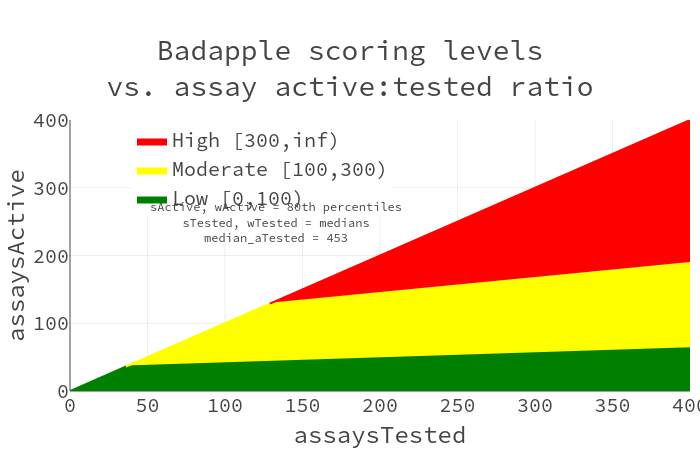
\includegraphics[width=\textwidth]{figures/badapple/badapple_formula.png}
	\caption{Badapple score dependence on assay-active and assay-tested statistics}
	\label{fig:BA_01}
\end{figure}

In figure \ref{fig:BA_01}, the color bands indicate the ranges of Badapple scores: low, moderate and high. It is clear that the score is not dependent only on the BA, i.e. ratio of actives to tested, since then the range boundaries would be straight lines through the origin. Rather, when the aTested is below a certain threshold (i.e. the weight of evidence is insufficient), moderate or high scores are disallowed. Below another threshold, high scores are disallowed. In this figure, the substance and well terms are held constant. Given the three-way symmetry of the Badapple formula, the corresponding figure for substance and well statistics would reflect the same properties.

\subsection{Statistical, Bayesian learning}

The Badapple formula is computationally simple, but combines some powerful features. Understanding its relationship to other statistical methods is important for comprehensibility, interpretation and to make best use of the methodology more generally. As one notable comparison, the Badapple formula shares some properties with the Internet Movie Database (IMDb) score (equation \ref{eq:ba_imdb}) used to rank movies in its “Top 250”\cite{IMDb_undated-ci}.

\begin{equation}
score = \frac{vR}{v + m} * \frac{mC}{v + m}
\label{eq:ba_imdb}
\end{equation}
where
\begin{itemize}
\item[] R = average rating for the movie \\
v = votes for the movie \\
m = minimum votes to be in Top 250 (currently 25,000) \\
C = the mean vote across the whole report (currently 7.0) \\
\end{itemize}

In particular, the use of the minimum-votes expression has a similar effect in devaluing high BAs if the weight of evidence is relatively low. IMDb describes their score as a “Bayesian Estimate” (BE). Although neither Badapple nor IMDb makes use of Bayes’ theorem, it may be both justified and explanatory to represent these methods as Bayesian-like. Badapple shares some key features of Bayesian approaches: (1) absence of any assumed probability distribution, and (2) by iterative learning cycles, new data can be used to continually improve the prediction model. Badapple also reflects systematic skeptical bias, meaning restricting the number of high scores using weight of evidence as a marker of confidence, because in the domain of bioassay data analysis, a semi-automated endeavor requiring human judgment, there is a limit to the number of red flags which can be readily processed.

\subsection{Knowledge management and “thoroughly conscious ignorance”}

While Badapple is robust to noise, it also is completely reliant on both the quality and coverage of the empirical data. If the data does not contain evidence for a given structure, for example, the Badapple score will be zero, representing “no indication”. If the data contains duplicate results, the scores are degraded, since accurate BAs depend on accurate counting. Obviously, multiple positive results in identical assays, or assays for identical targets, are not indicative of promiscuity. The logical implication of being data driven is that without data there is no knowledge. However, to quote James Clerk Maxwell: “Thoroughly conscious ignorance is the prelude to every real advance in science.” By avoiding a prejudiced guess, an algorithm or scientist can be prepared for the arrival of new information.

\subsection{BARD and the Badapple plugin}

\emph{Enterprise bioassay analysis}

The BioAssay Research Database (BARD)\cite{De_Souza2014-rf} is designed as a resource for bioassay data and particularly its use by researchers in exploratory data analysis and knowledge discovery. Accordingly, BARD includes a powerful and extensible computational platform whereby plugins can be deployed and integrated seamlessly with the BARD public REST API\cite{De_Souza2014-rf}. Badapple was chosen as the first “exemplar” BARD plugin (Additional file 1), based on the scientific value of promiscuity modeling and the direct relevance to bioassay data analysis. The BARD project began in March 2012 and the first version of the Badapple plugin was released in Sept 2012, using training data from PubChem. Subsequent versions of the plugin have used data directly from BARD, and PubChem assay IDs (AID) were replaced by BARD experiment IDs (EID). This migration was a positive step in elevating the semantic rigor of Badapple, toward systematic de-duplication of assays.

\subsection{BARD/MLP Badapple data analysis}

\emph{The privileged and notorious few}

Approach Rigorous classification of assays and targets in bioassay databases has been a continuing challenge, with efforts ongoing by the projects BAO and BARD. However, MLP assays were selected for scientific merit and therefore tend to be non-redundant. Likewise, MLSMR is a non-redundant screening library by design. Accordingly, for this study, and because Badapple was originally designed for HTS bioassay data analysis, the dataset chosen for analysis consists of MLP HTS assays and MLSMR compounds. Additionally, as the community may be familiar with this data, this well characterized dataset can facilitate interpretation and replication of results.
Output scores and statistics Complete Badapple output is provided in the Additional file 2 for all scaffolds in for the BARD-based version “bard1”. These results include computed Badapple scores, plus assay, substance and sample statistics for each scaffold. PostgreSQL databases used in this study are also available via links provided in Additional file 2. The R code used for analysis is also provided, and top scoring scaffolds are presented in table \ref{table:BA_Fig2}.

\begin{table}
\caption{Top promiscuous scaffolds, ranked by Badapple score (see Additional file 2 for full statistics)}
\begin{center}
\begin{tabular}{ |c|c|c|c| } 
\hline
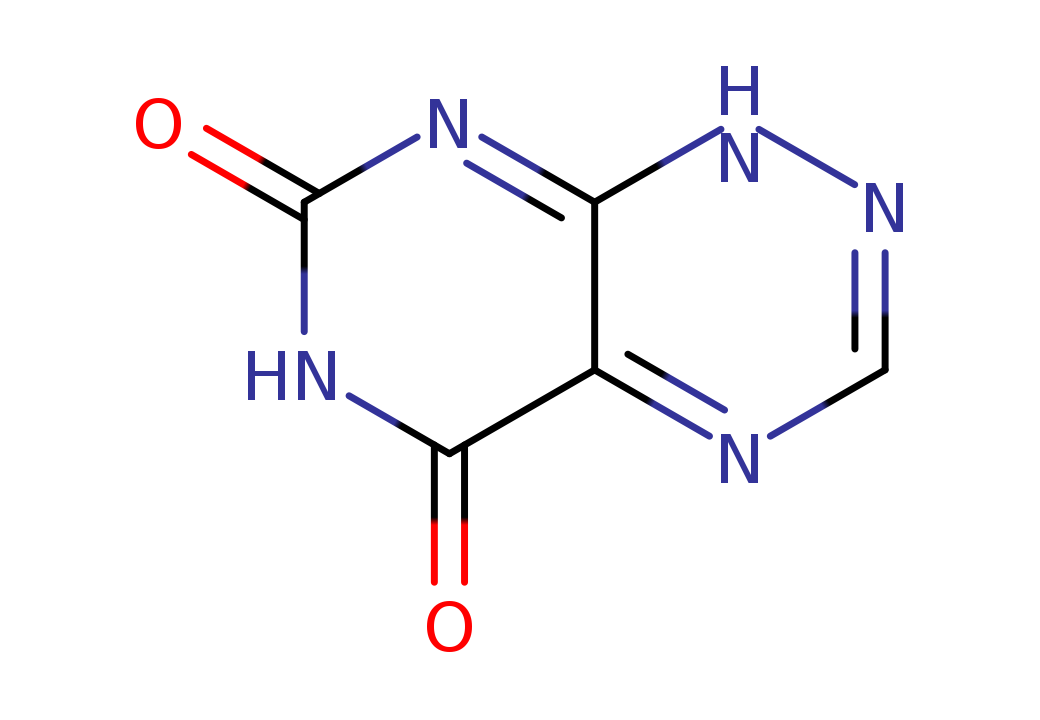
\includegraphics[align=t,width=0.2\textwidth]{data/badapple/Fig2_scaf_01.png} 
& 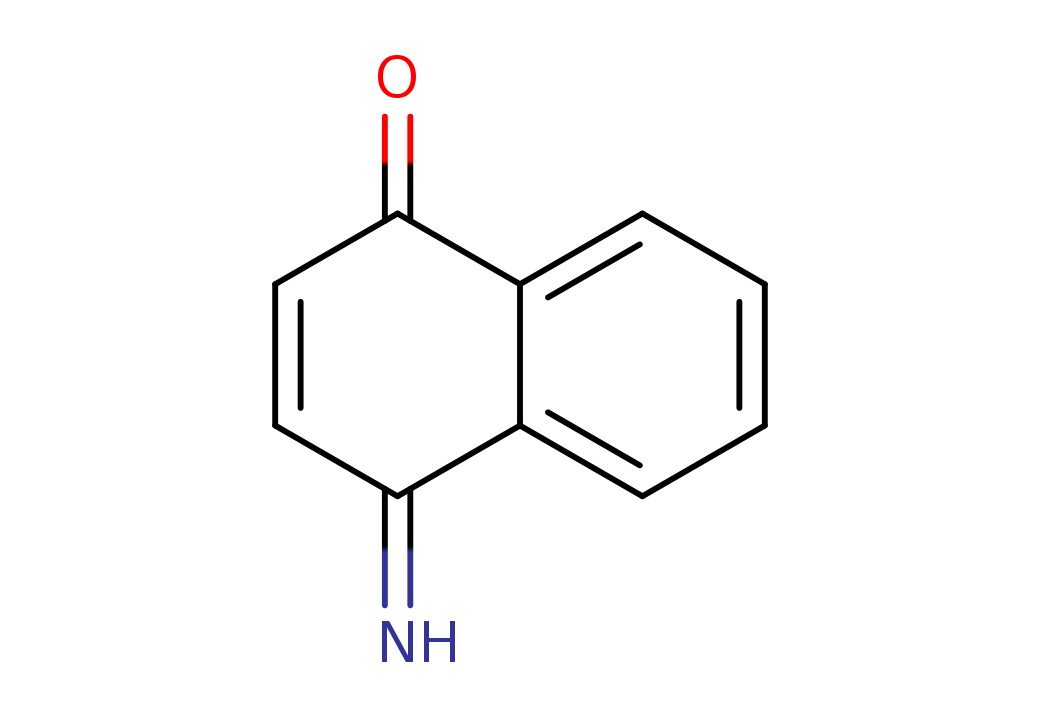
\includegraphics[align=t,width=0.2\textwidth]{data/badapple/Fig2_scaf_02.png}
& 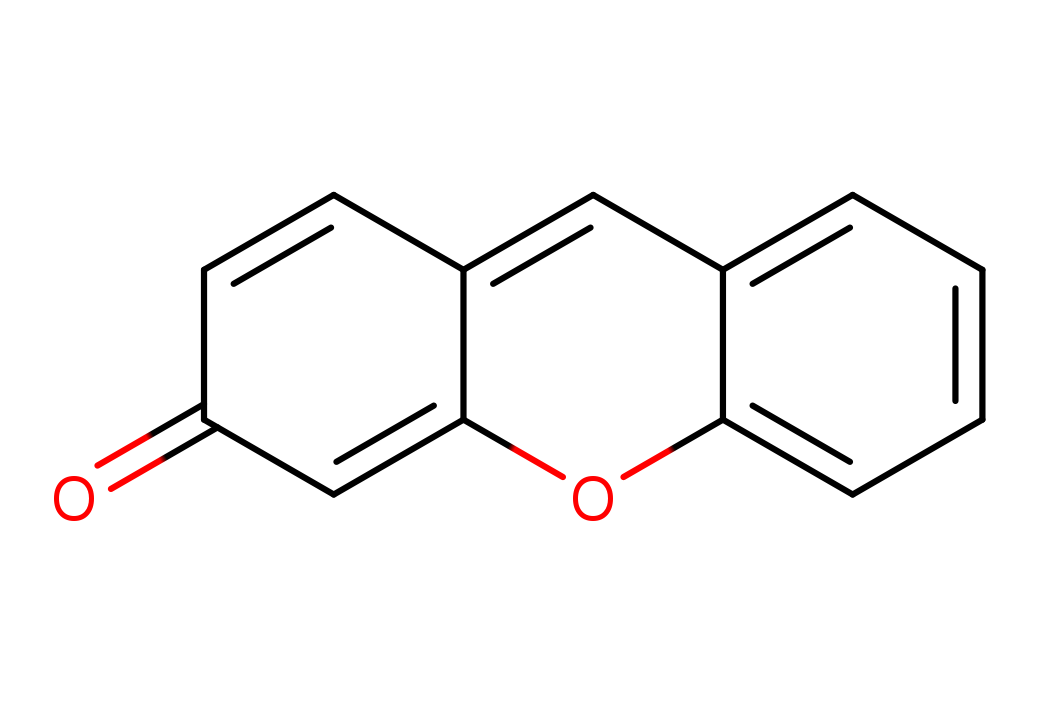
\includegraphics[align=t,width=0.2\textwidth]{data/badapple/Fig2_scaf_03.png}
& 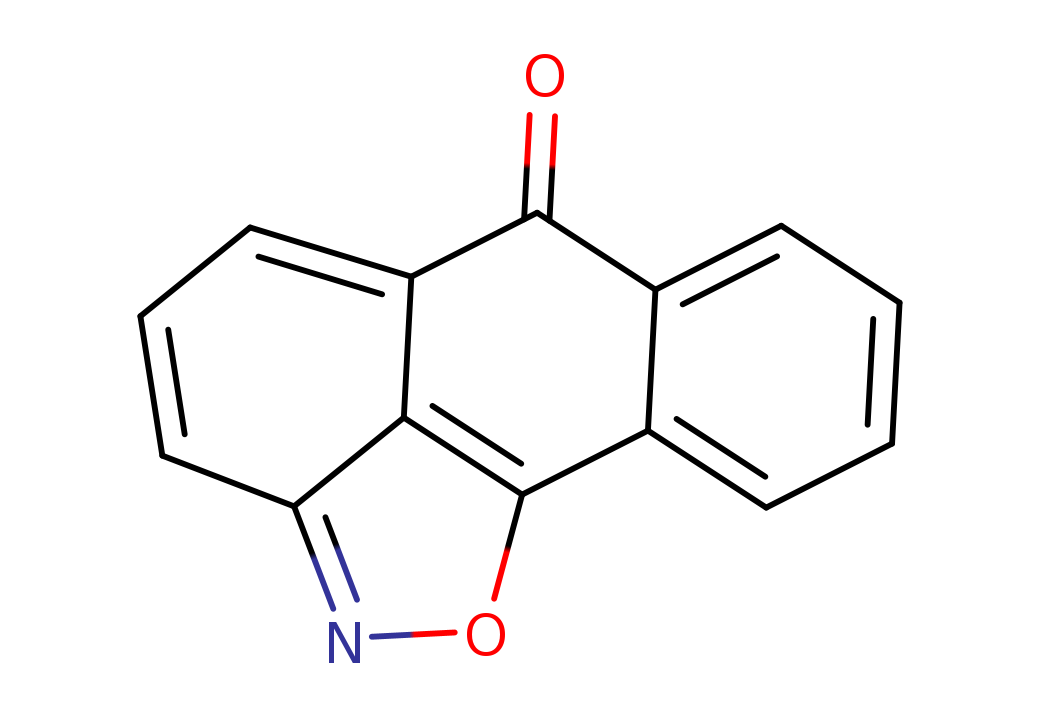
\includegraphics[align=t,width=0.2\textwidth]{data/badapple/Fig2_scaf_04.png} \\
\texttt{2544} & \texttt{2445} & \texttt{2413} & \texttt{2315} \\
\hline
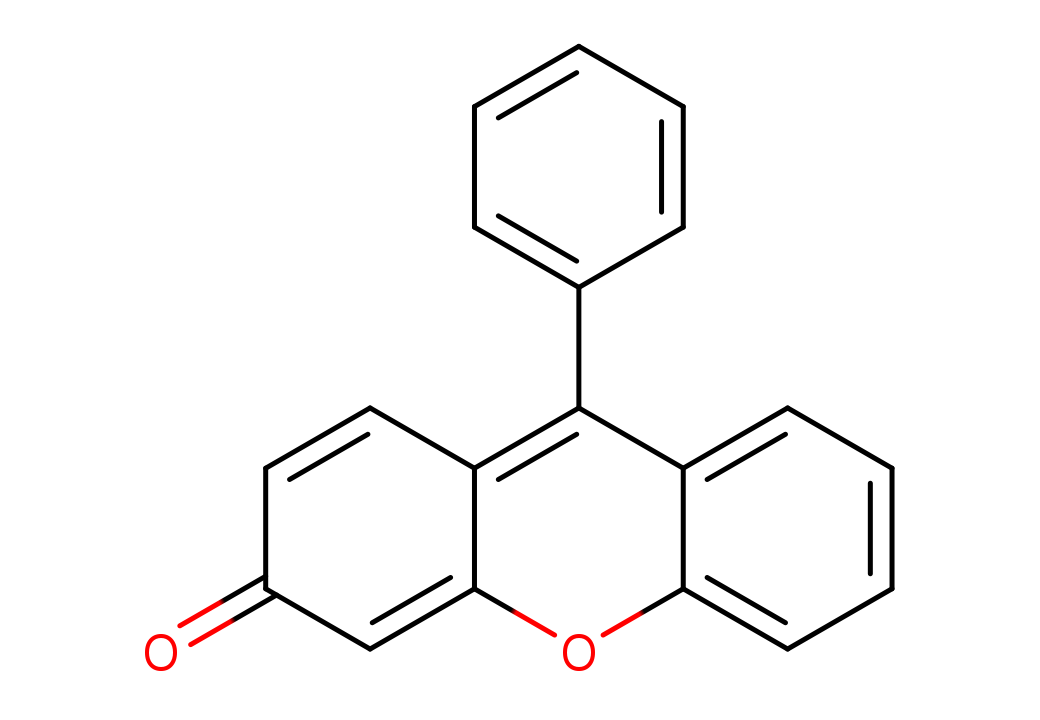
\includegraphics[align=t,width=0.2\textwidth]{data/badapple/Fig2_scaf_05.png} 
& 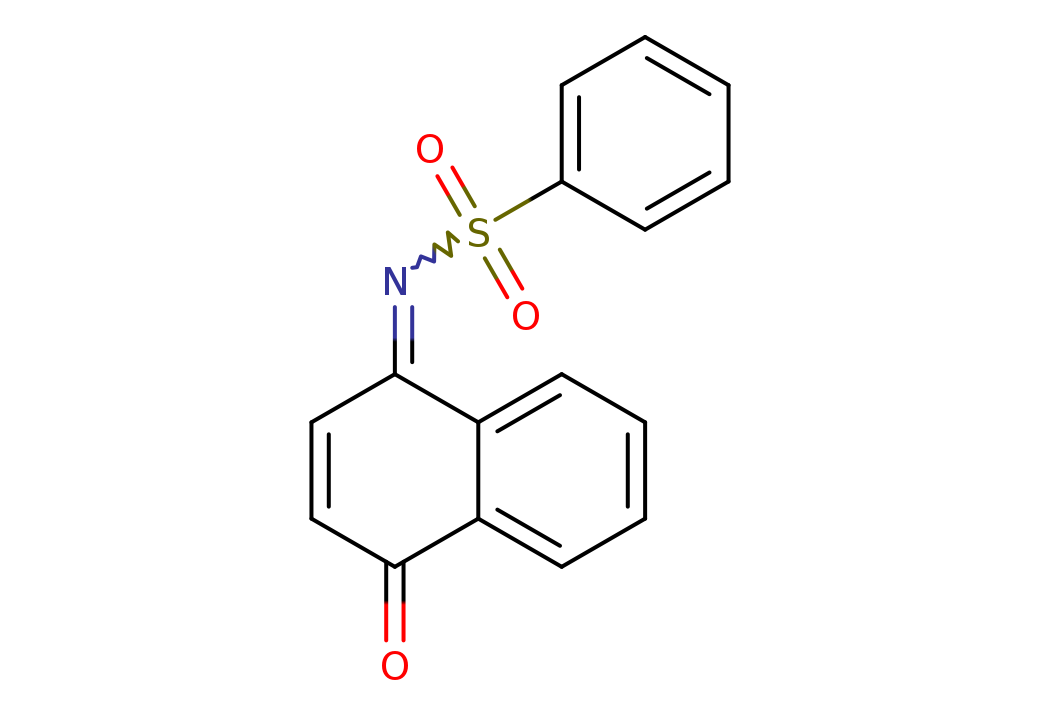
\includegraphics[align=t,width=0.2\textwidth]{data/badapple/Fig2_scaf_06.png}
& 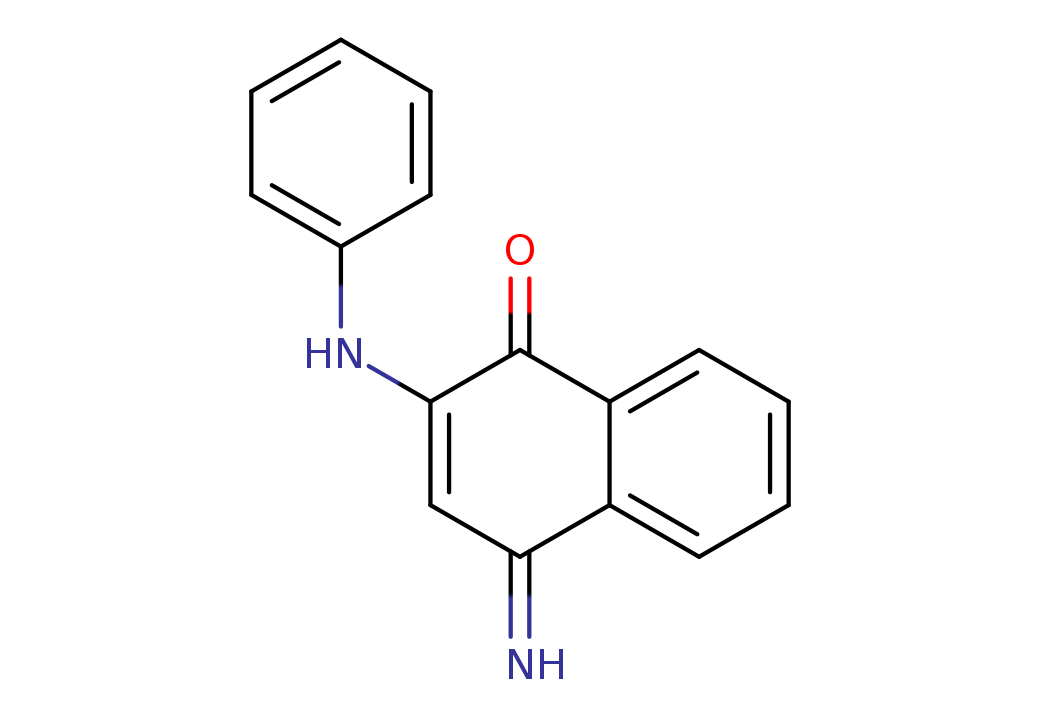
\includegraphics[align=t,width=0.2\textwidth]{data/badapple/Fig2_scaf_07.png}
& 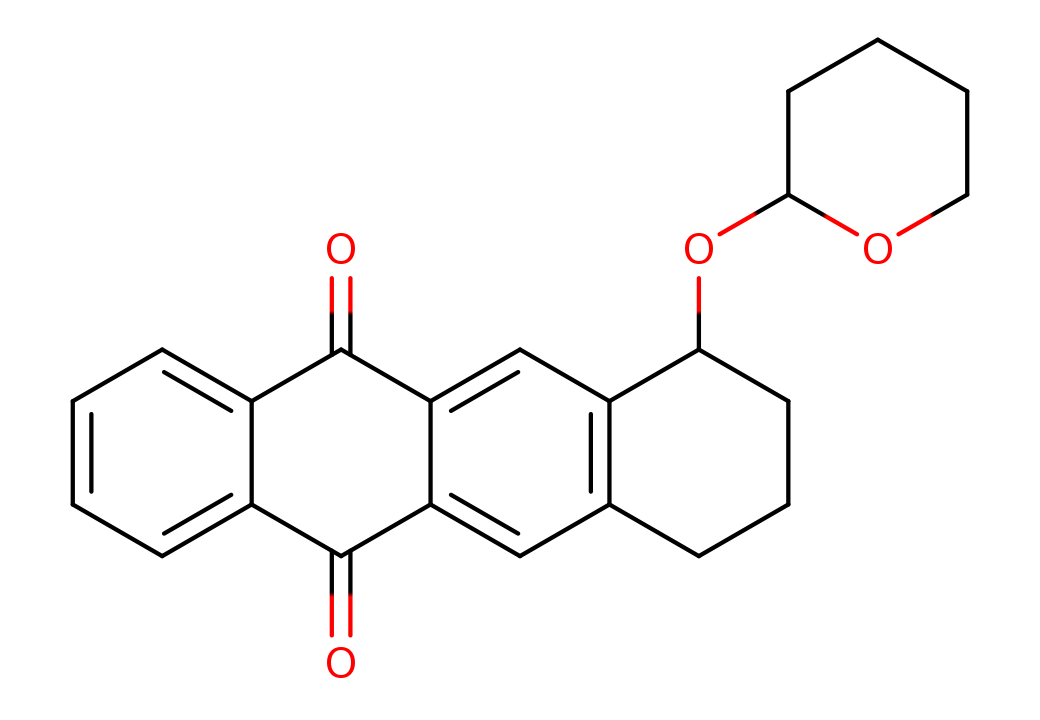
\includegraphics[align=t,width=0.2\textwidth]{data/badapple/Fig2_scaf_08.png} \\
\texttt{2182} & \texttt{2147} & \texttt{1996} & \texttt{1888} \\
\hline
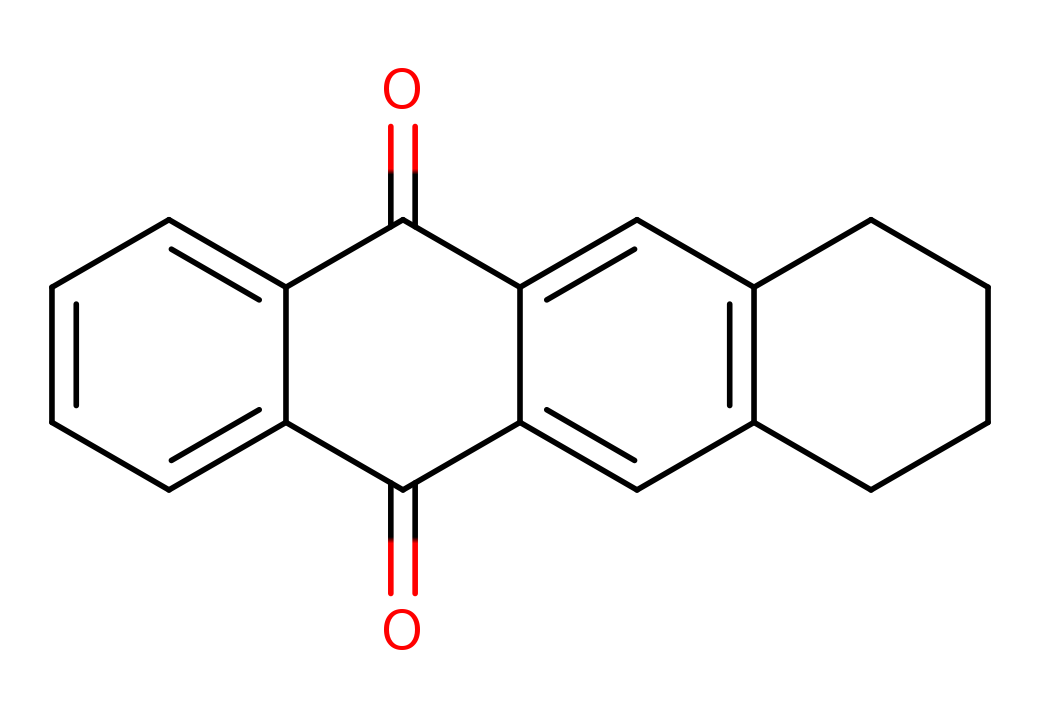
\includegraphics[align=t,width=0.2\textwidth]{data/badapple/Fig2_scaf_09.png} 
& 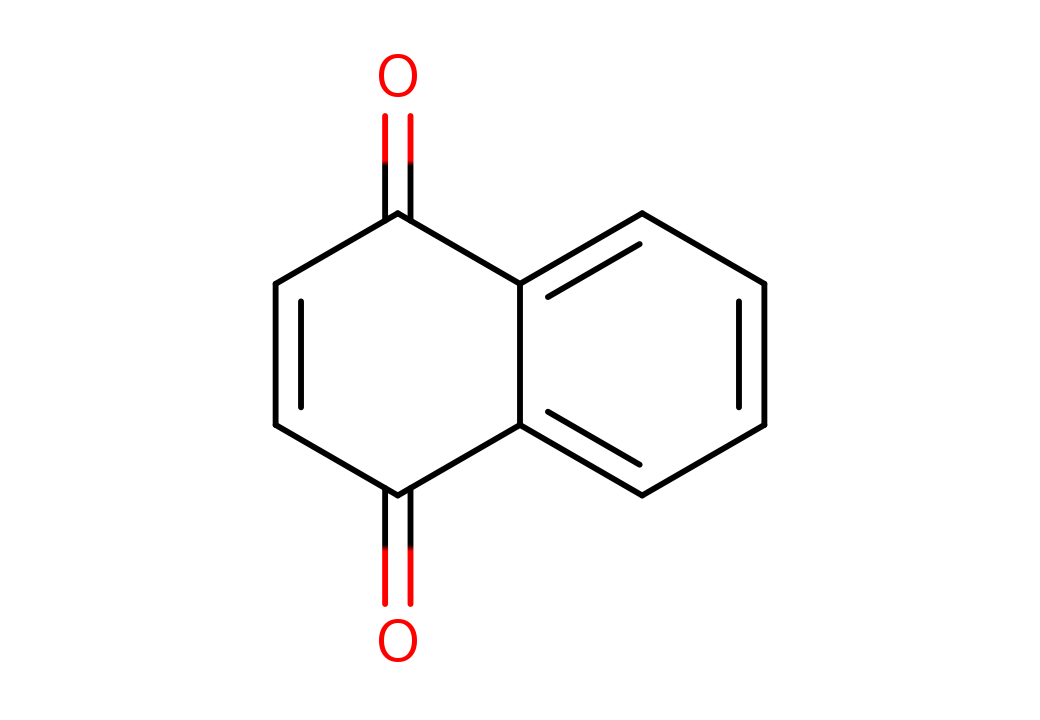
\includegraphics[align=t,width=0.2\textwidth]{data/badapple/Fig2_scaf_10.png}
& 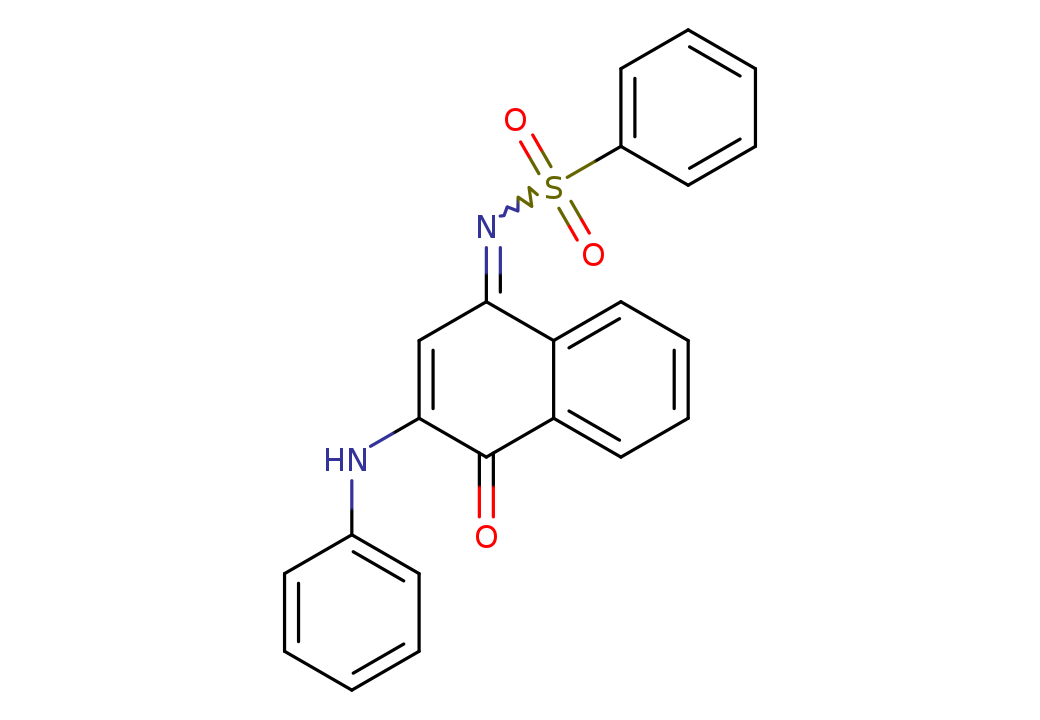
\includegraphics[align=t,width=0.2\textwidth]{data/badapple/Fig2_scaf_11.png}
& 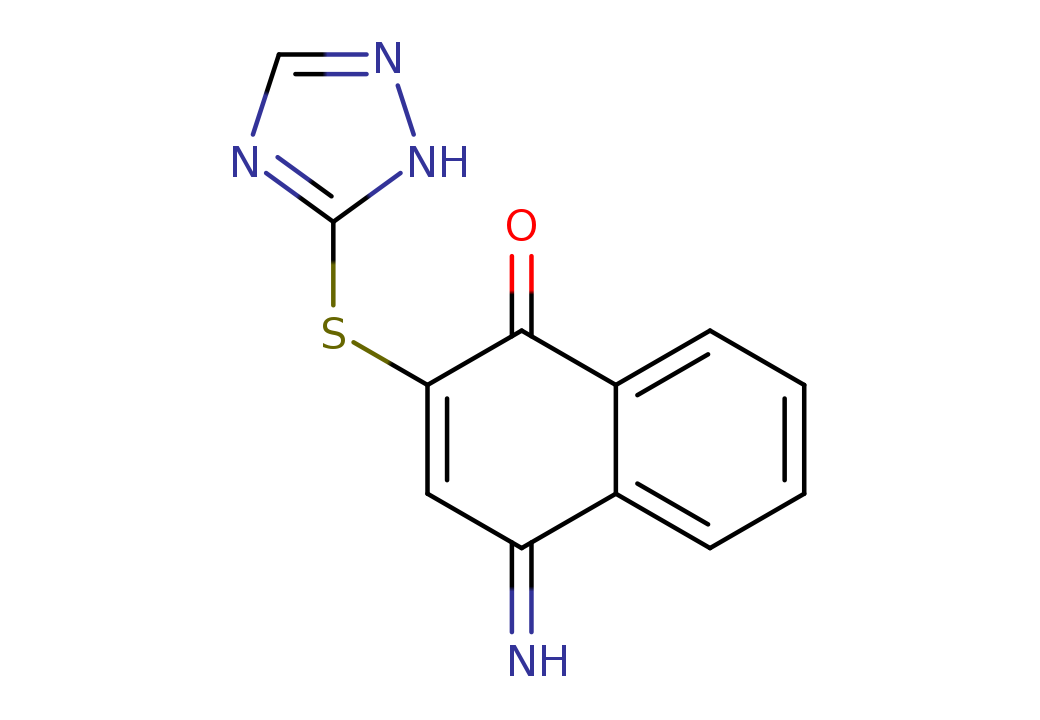
\includegraphics[align=t,width=0.2\textwidth]{data/badapple/Fig2_scaf_12.png} \\
\texttt{1888} & \texttt{1707} & \texttt{1631} & \texttt{1443} \\
\hline
\end{tabular}
\end{center}
\label{table:BA_Fig2}
\end{table}

The total scaffold count is 146,024, of which 383 (0.3 \%) are high scoring, 1692 (1.2 \%) are moderate, and the remaining 143,949 (98.6 \%) are low scoring. The distribution is shown in figure \ref{fig:BA_03}. While the cutoff values are arbitrary (and rooted in observed distributions), they are informed by the overall need to efficiently support scientific workflows. Too many “red flags” would increase the chance of false alarms and would themselves be increasingly costly to analyze. Users with sufficient time should not rely on cutoffs but investigate as many high and moderate scores as time permits.

\begin{figure}
	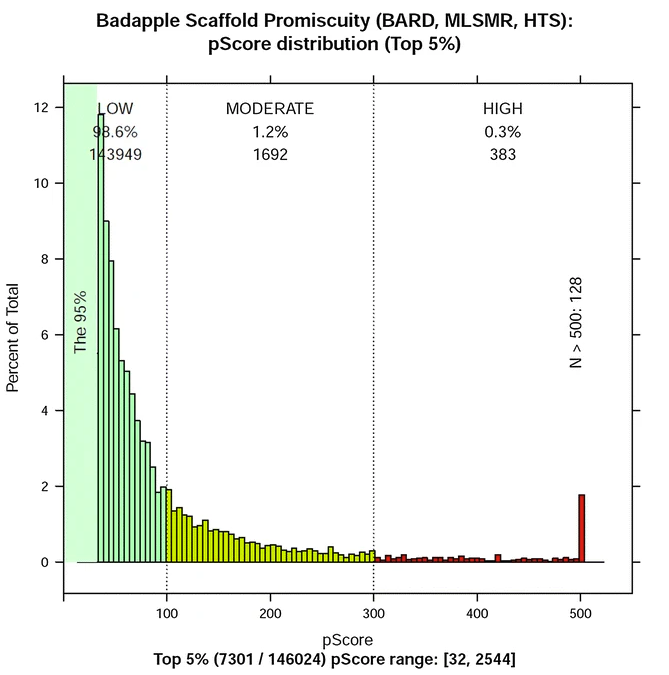
\includegraphics[width=\textwidth]{figures/badapple/Badapple_Fig3.png}
	\caption{Promiscuity score distribution}
	\label{fig:BA_03}
\end{figure}

Although there are relatively few high scoring scaffolds, those “privileged” few account for a disproportionate share of the bioactivity in the dataset (i.e. samples deemed active by the assay). Figure 4 illustrates this skewness via receiver operating characteristic (ROC) curves, which plot the percentage of active samples retrieved, with the horizontal axis the top scaffolds (top 5 \%) in ranked by score. Overall, 50 \% of all bioactivity is associated with 1.4 \% (1979) of the scaffolds. (By “50 \% of all bioactivity” we mean 50 \% of all active samples.) For drug-scaffolds, 50 \% of all bioactivity is associated with 2.8 \% (54) of the scaffolds. These data support the Badapple approach of identifying a relative few scaffolds for scrutiny, partly because human investigators have limited time, but also because nature appears to confer special properties to a relative few.

\begin{figure}
	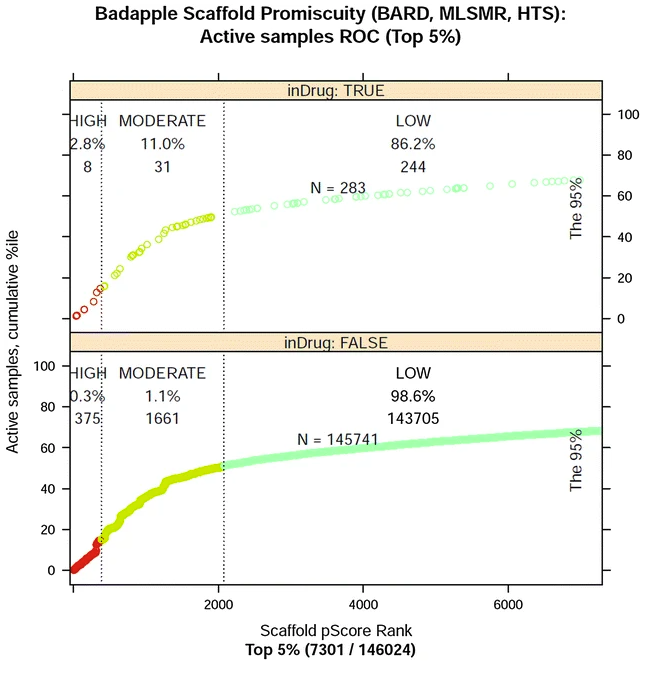
\includegraphics[width=\textwidth]{figures/badapple/Badapple_Fig4.png}
	\caption{ROC curves, total bioactivity versus ranked top scaffolds for top 5 \%}
	\label{fig:BA_04}
\end{figure}


\subsection{Prediction, validation, and history}

\emph{“Those who fail to learn from history are doomed to repeat it”: George Santayana}

The Badapple algorithm is intended as a tool to quickly assess the likely promiscuity of HTS hits or arbitrary compounds of interest. It has been noted that predicting the future is hard. Fortunately, if a future instance is very similar to a prior instance, studying history can suffice. History can also be hard since it requires good information, often a precious commodity. Supervised machine learning (ML) predictive models are also trained on historical data. ML models can be powerful and useful, but are prone to overfitting and often uninterpretable. In contrast, a Badapple score is a statistic, an algebraic function of empirical, historical data.

To validate Badapple we used retrospective datasets to indicate whether scores generated in the past would have been predictive, in other words, consistent with subsequent bioassay findings. The scores and rankings of scaffolds were compared using conventional Pearson correlation and also Spearman rank correlation. Spearman rank is included since for operational purposes where only top-X hits can be investigated, rank may be more important than raw score. We compare scaffolds for which older data yield high scores and new data exists. By comparing the newer, updated scores with the older scores for this subset, we can evaluate the usefulness of Badapple. Refer to tables \ref{table:ba_cmp_scaf}, \ref{table:ba_cmp_corr}, \ref{table:ba_cmp_xval} and \ref{table:ba_cmp_retro} for this analysis.

\begin{table}
\caption{Badapple datasets}
\begin{center}
\begin{tabular}{ |l|c|c|c|c|c|c|l| } 
\hline
& \textbf{\#scafs} & \textbf{Tested} & \textbf{Nonzero} & \textbf{\#assy} & \textbf{Activities} & \textbf{Date} & \textbf{Source} \\
\hline
Bard1 & 146,024 & 141,642 & 54,136 & 510 & 30M & 2013-01 & BARD \\
Bard2 & 143,098 & 137,668 & 52,328 & 383 & 46M & 2014-06 & BARD \\
Pc1 & 143,098 & 141,533 & 60,200 & 822 & 223M & 2014-06 & PubChem \\
Pc2 & 143,098 & 125,940 & 50,912 & 527 & 113M & 2010-12 & PubChem \\
\hline
\end{tabular}
\end{center}
\label{table:ba_dsets}
\end{table}


BARD assay counts are experiment counts. Tested means bioassay data exist. Nonzero means tested with nonzero scores


\begin{table}
\caption{Badapple dataset comparison: scaffolds in common (total/non-zero)}
\begin{center}
\begin{tabular}{ |r|c|c|c| } 
\hline
& \textbf{Bard2} & \textbf{Pc2} & \textbf{Pc1} \\
\hline
\textbf{Bard1} & 141896 ; 41,218 & 141,629 ; 49,844 & 141,629 ; 43,951 \\
\hline
\textbf{Bard2} & & 142,817 ; 43,083 & 142,817 ; 40,463 \\
\hline
\textbf{Pc2} & & & 143,087 ; 47,252 \\
\hline
\end{tabular}
\end{center}
\label{table:ba_cmp_scaf}
\end{table}



\begin{table}
\caption{Badapple dataset comparison: PScore correlation, Pearson/Spearman-rank}
\begin{center}
\begin{tabular}{ |r|c|c|c| } 
\hline
& \textbf{Bard2} & \textbf{Pc2} & \textbf{Pc1} \\
\hline
\textbf{Bard1} & 0.85 ; 0.73 & 0.95 ; 0.89 & 0.92 ; 0.85 \\
\hline
\textbf{Bard2} & & 0.86 ; 0.69 & 0.85 ; 0.72 \\
\hline
\textbf{Pc2} & & & 0.96 ; 0.87 \\
\hline
\end{tabular}
\end{center}
\label{table:ba_cmp_corr}
\end{table}


As an additional validation, the global compound set (389,533) was subjected to randomly partitioned fivefold cross validation. For each fold, 1/5th of the dataset
served as test set, with 4/5th as training set. By recalculating all scores for the training set scaffolds, using only activity data for training set compounds, we
simulated the situation where test set compounds are new and unknown. For each compound, we associate the score from its highest scoring scaffold. For each fold,
compounds which previously had associated Badapple scores may not, since the training set is reduced relative to the original Badapple training set. This can be
interpreted as a loss of predictive scope. The Pearson correlation was calculated for each fold, for all test compounds, with those unscored assigned a score of
zero, to reflect overall predictive power from each training set. Each correlation was approximately 0.9, indicating strong and consistent predictive power. These
results are summarized in table \ref{table:ba_cmp_corr}.

\begin{longtable}{ccccc}
\caption{Retrospective comparison of high scores, pc2 versus pc1}\\
\hline
\textbf{Scaffold} & \textbf{pscore\_pc2} & \textbf{pscore\_pc1} & \textbf{pscore\_diff} & \textbf{wTested\_diff} \\
\hline
\endfirsthead
\multicolumn{5}{c}
{\tablename\ \thetable\ -- \textit{Continued from previous page}} \\
\hline
\textbf{Scaffold} & \textbf{pscore\_pc2} & \textbf{pscore\_pc1} & \textbf{pscore\_diff} & \textbf{wTested\_diff} \\
\hline
\endhead
\hline \multicolumn{5}{r}{\textit{Continued on next page}} \\
\endfoot
\endlastfoot

\includegraphics[width=60px]{data/badapple/scaf_01.png} & \makecell[{{m{1cm}}}]{436} & 395 & 41 & 7,234,388 \\

\includegraphics[width=60px]{data/badapple/scaf_02.png} & 374 & 343 & 31 & 5,511,793 \\

\includegraphics[width=60px]{data/badapple/scaf_03.png} & 443 & 369 & 74 & 2,644,122 \\
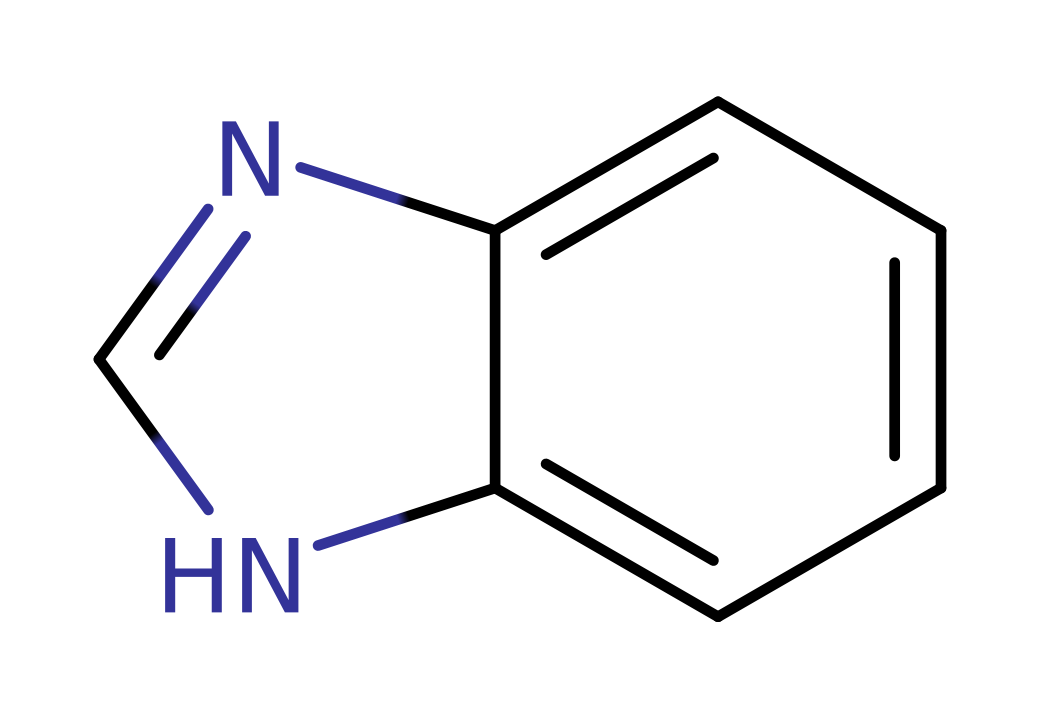
\includegraphics[width=60px]{data/badapple/scaf_04.png} & 432 & 392 & 40 & 1,701,524 \\
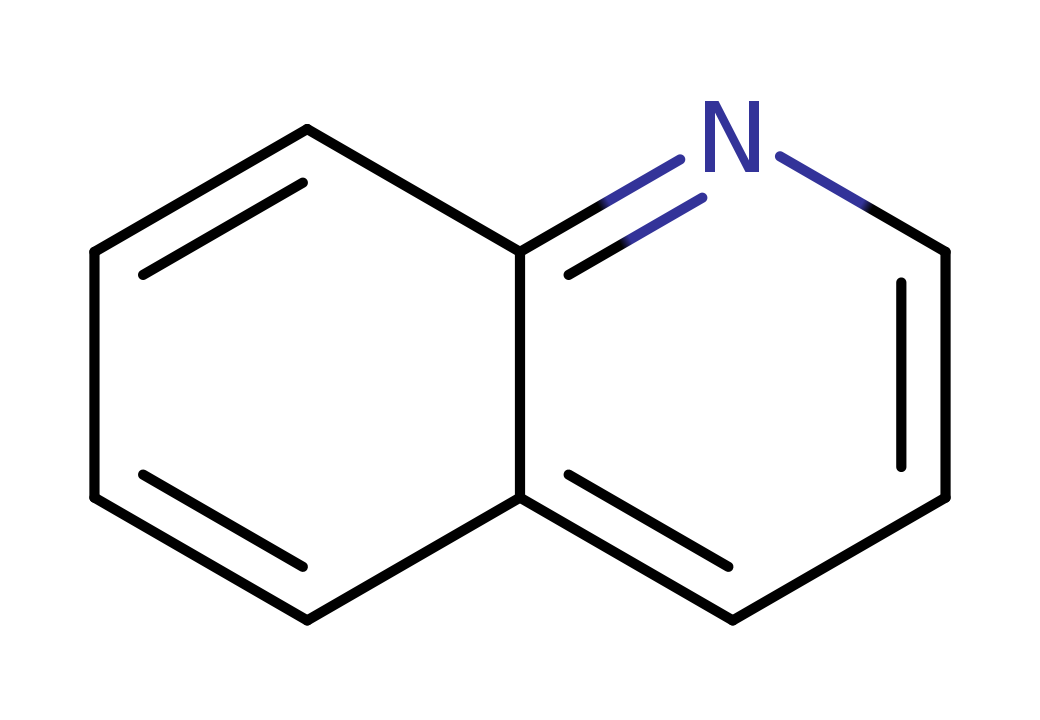
\includegraphics[width=60px]{data/badapple/scaf_05.png} & 578 & 468 & 110 & 1,652,980 \\
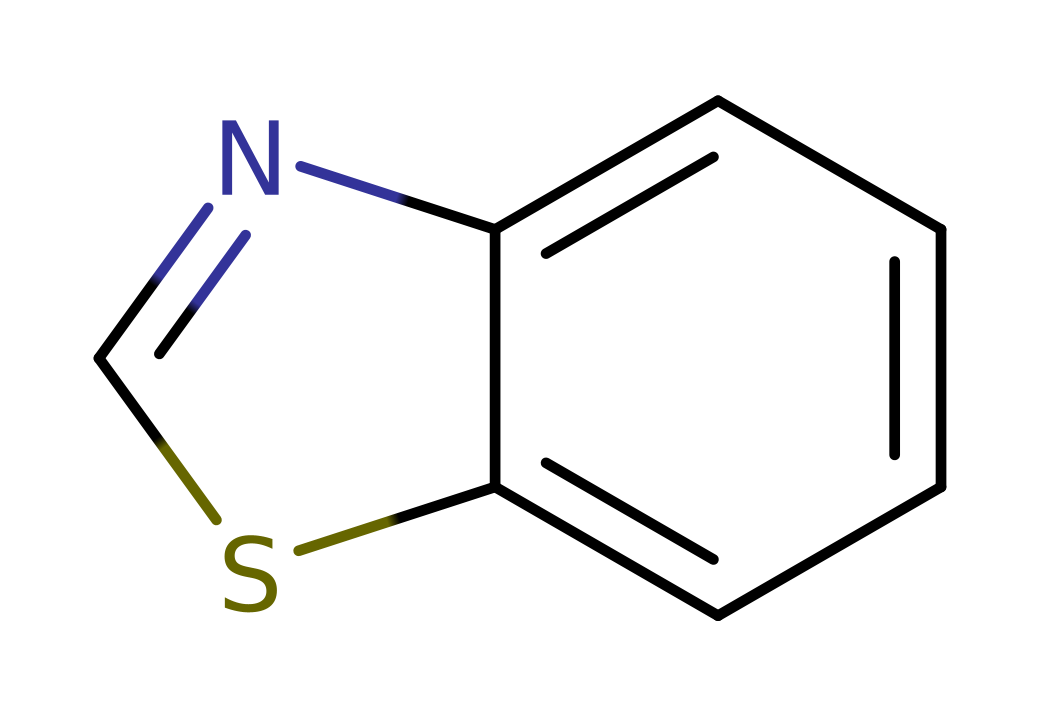
\includegraphics[width=60px]{data/badapple/scaf_06.png} & 618 & 627 & -9 & 1,019,584 \\
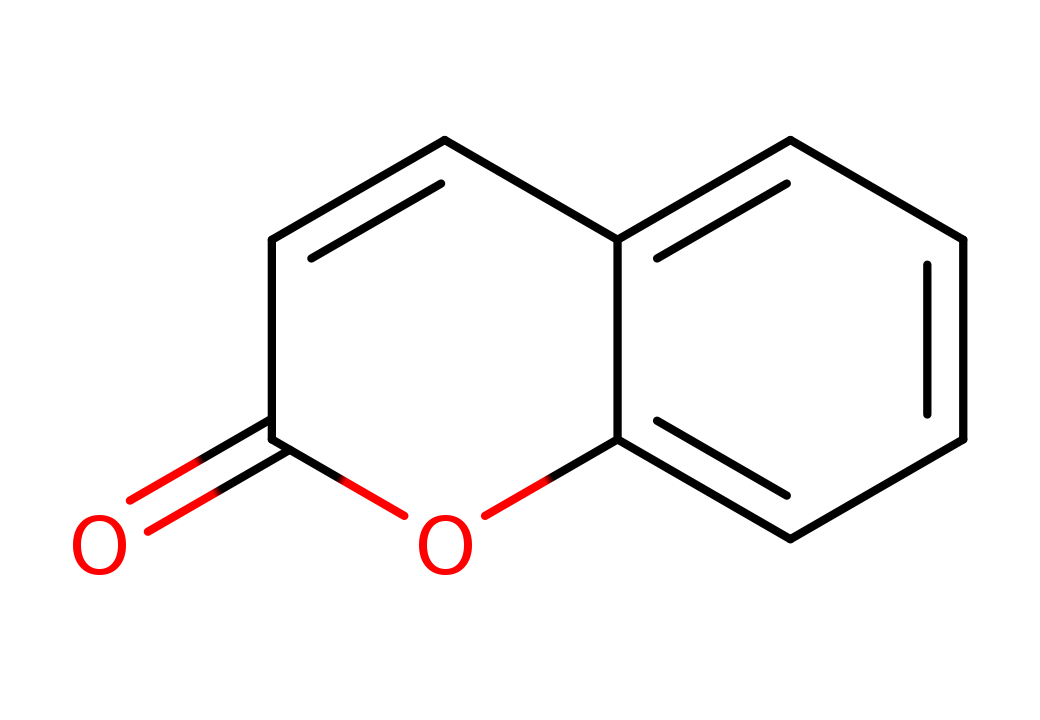
\includegraphics[width=60px]{data/badapple/scaf_07.png} & 375 & 315 & 60 & 899,779 \\
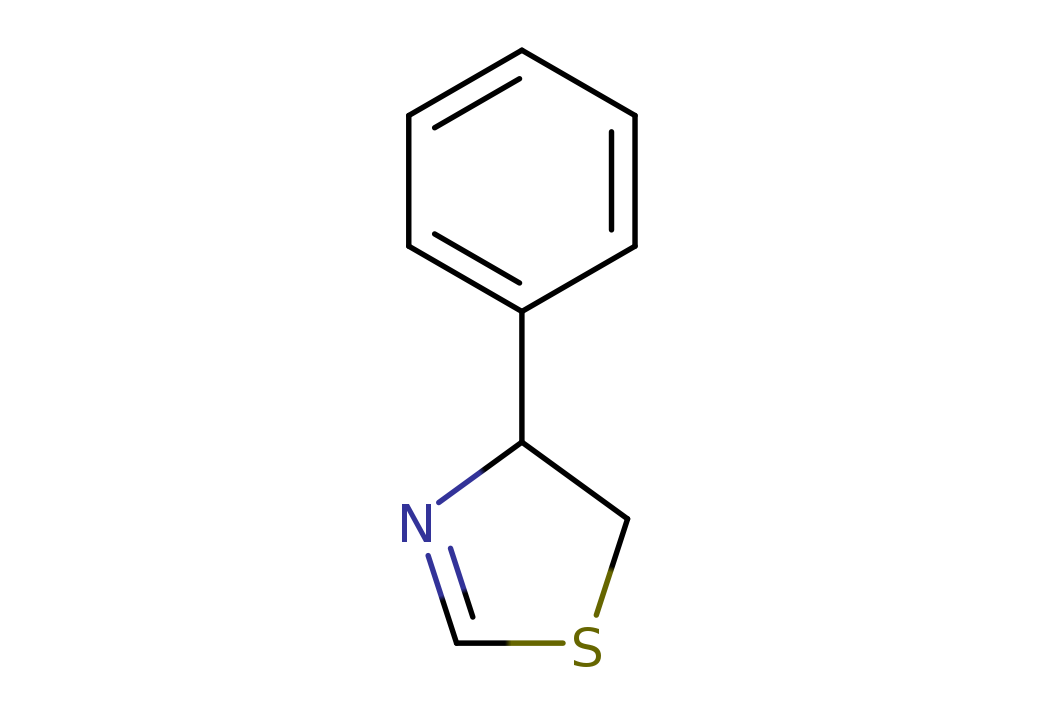
\includegraphics[width=60px]{data/badapple/scaf_08.png} & 463 & 366 & 97 & 654,420 \\
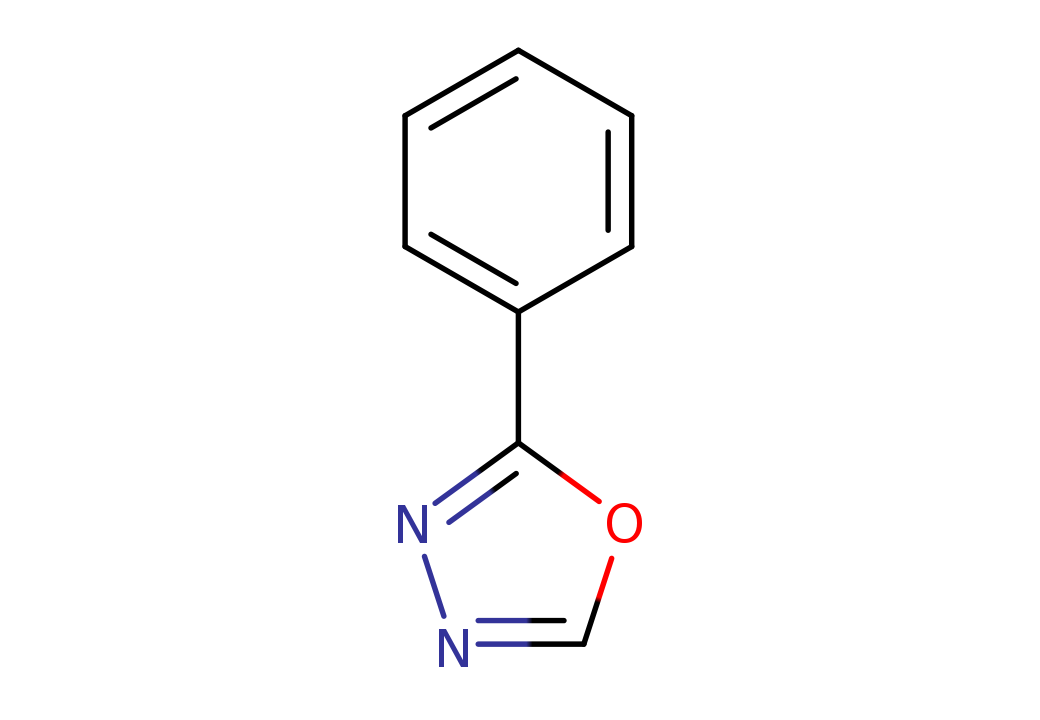
\includegraphics[width=60px]{data/badapple/scaf_09.png} & 365 & 361 & 4 & 524,438 \\
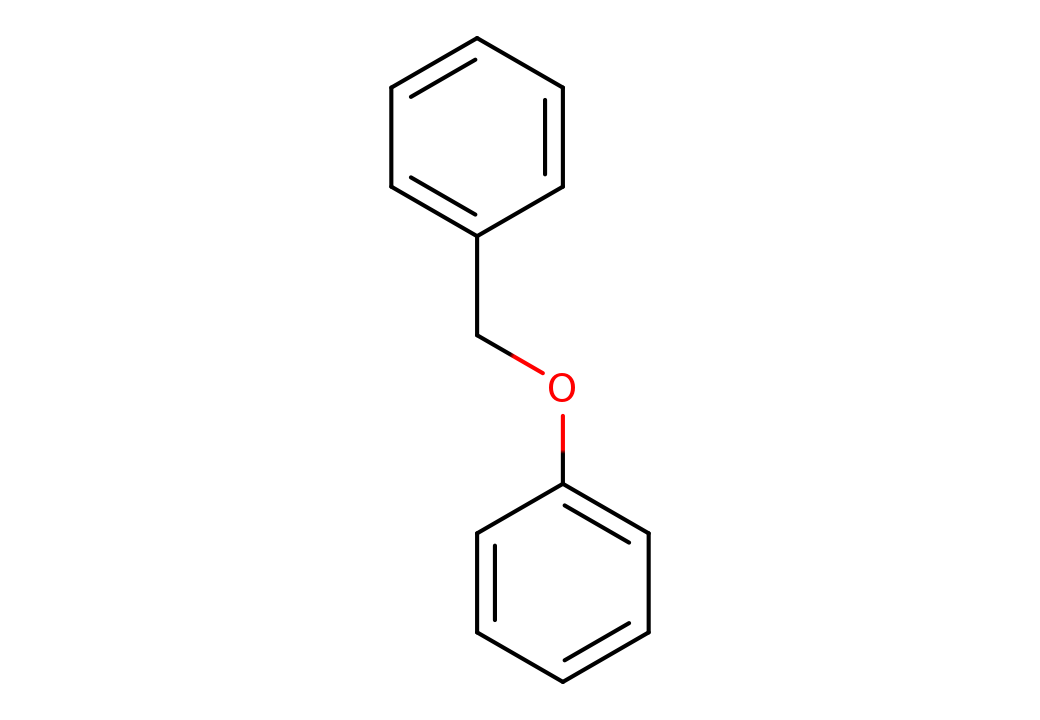
\includegraphics[width=60px]{data/badapple/scaf_10.png} & 461 & 367 & 94 & 496,504 \\
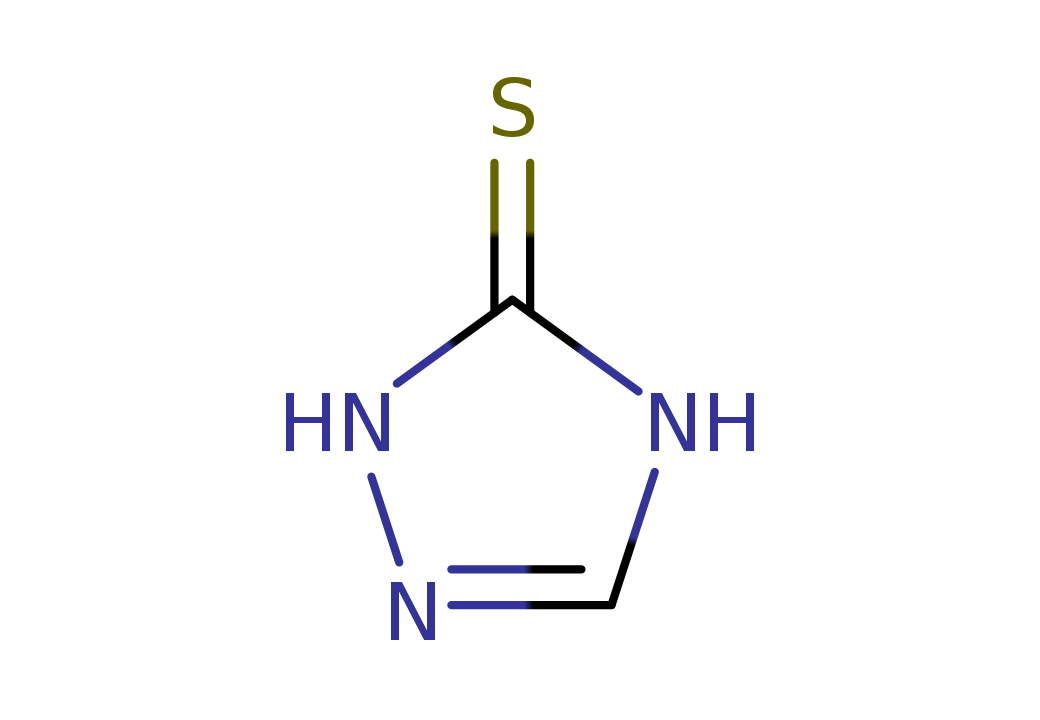
\includegraphics[width=60px]{data/badapple/scaf_11.png} & 358 & 303 & 55 & 422,280 \\
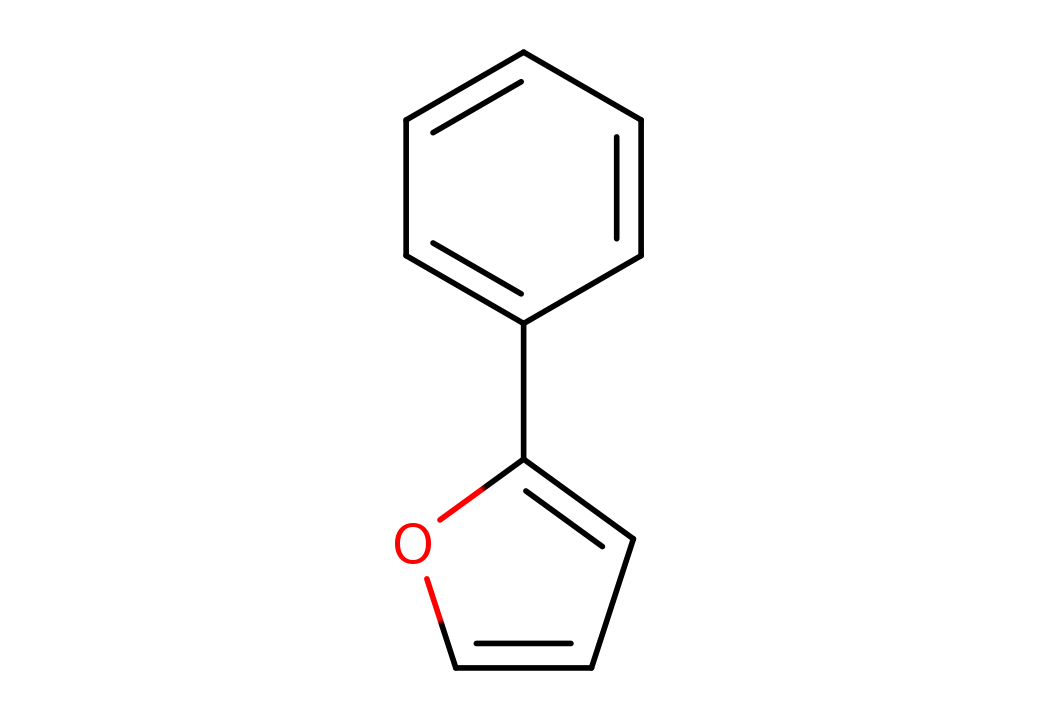
\includegraphics[width=60px]{data/badapple/scaf_12.png} & 805 & 696 & 109 & 376,575 \\
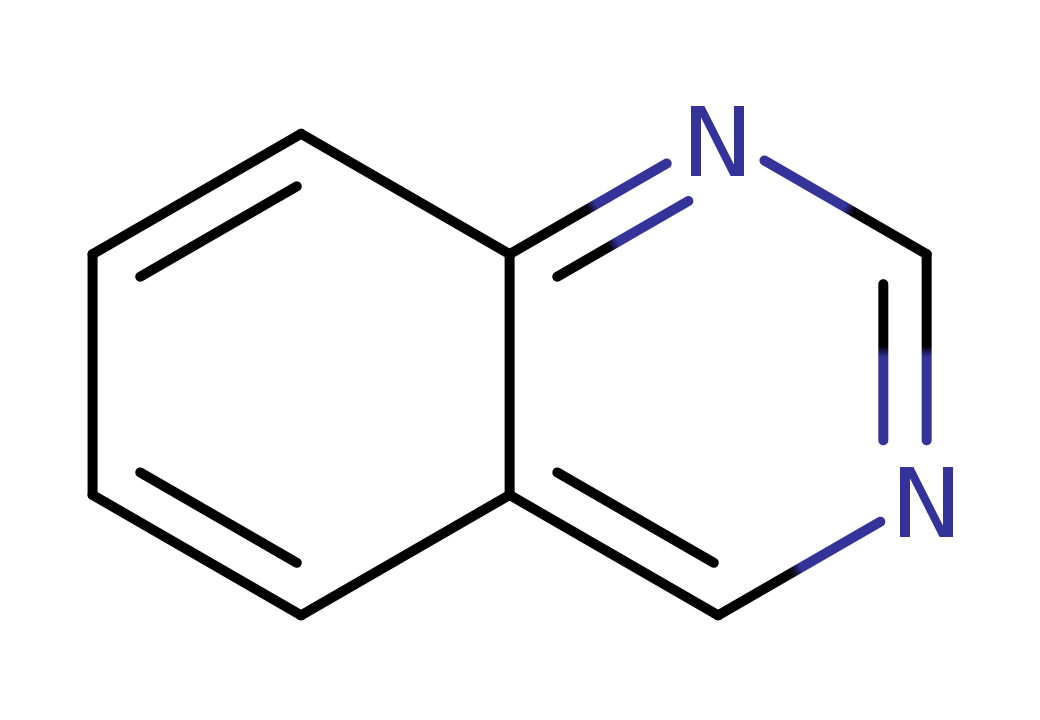
\includegraphics[width=60px]{data/badapple/scaf_13.png} & 403 & 331 & 72 & 358,012 \\
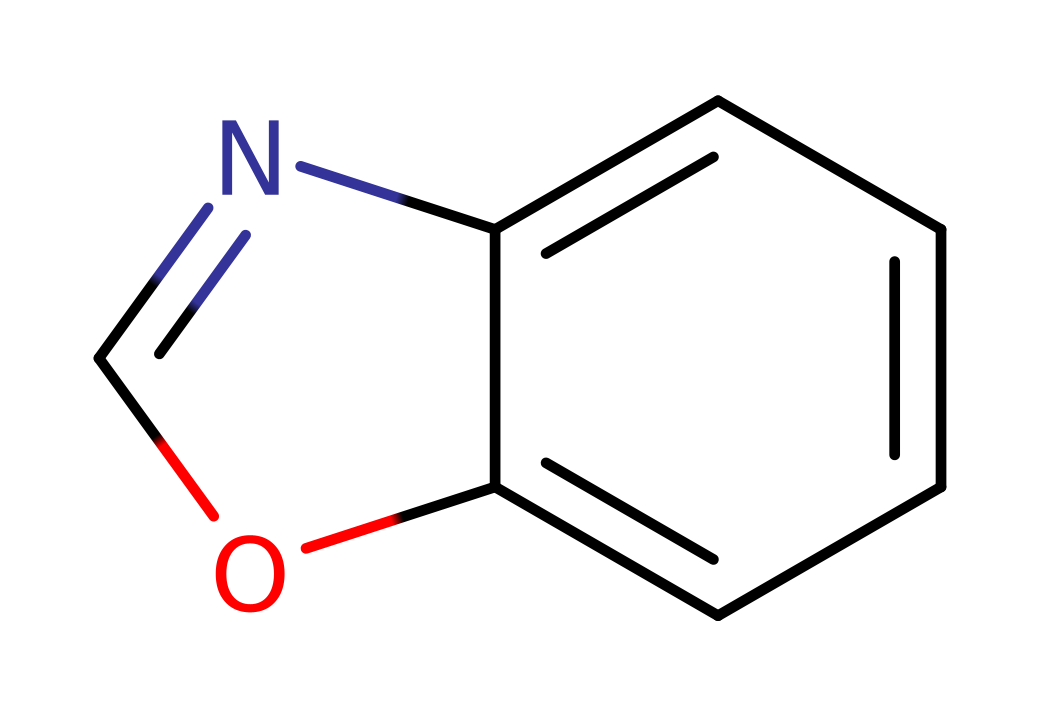
\includegraphics[width=60px]{data/badapple/scaf_14.png} & 459 & 487 & -28 & 319,746 \\
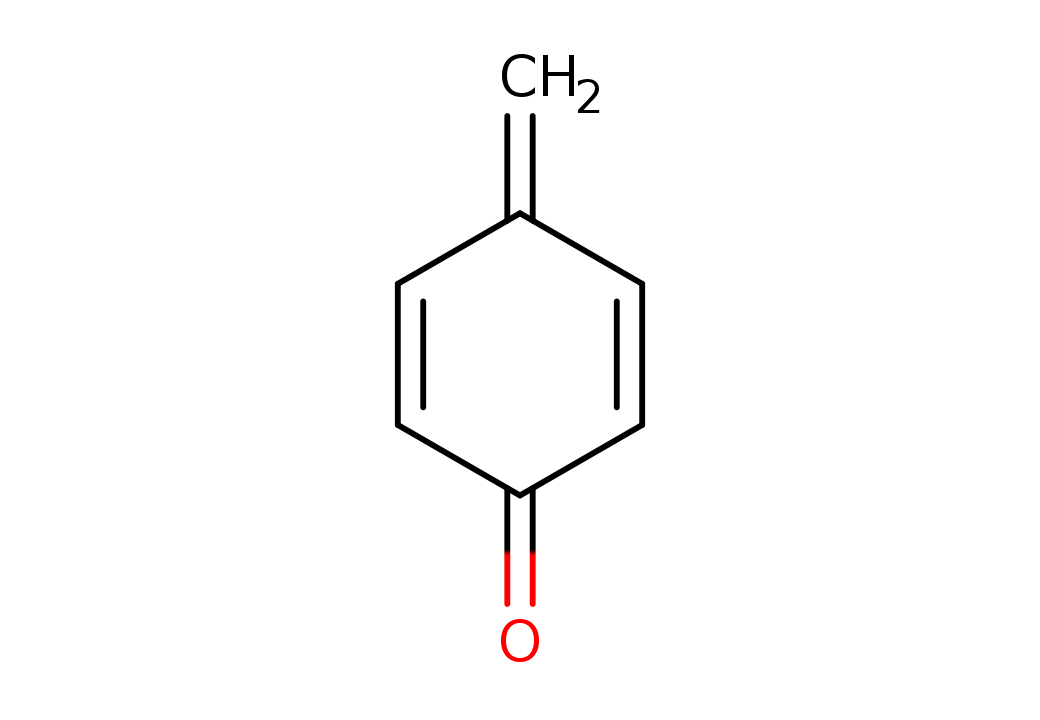
\includegraphics[width=60px]{data/badapple/scaf_15.png} & 841 & 721 & 120 & 318,307 \\
\hline
\label{table:ba_cmp_retro}
\end{longtable}


\begin{table}
\caption{K-fold cross validation (K = 5): Ntotal = 389,533, Pearson correlation, all test scores}
\begin{center}
\begin{tabular}{ |c|c|c|c| } 
\hline
\textbf{k} & \textbf{Ntrain} & \textbf{Ntest} & \textbf{Correlation} \\
\hline
1 & 311,540 & 77,993 & 0.895 \\
2 & 311,463 & 78,070 & 0.891 \\
3 & 311,652 & 77,881 & 0.898 \\
4 & 311,565 & 77,968 & 0.901 \\
5 & 311,454 & 78,079 & 0.903 \\
\hline
\end{tabular}
\end{center}
\label{table:ba_cmp_xval}
\end{table}


\begin{table}
\caption{Medchem analysis of selected high scoring, promiscuous scaffolds}
\begin{tabular}{p{0.3\linewidth}p{0.7\linewidth}}
\hline
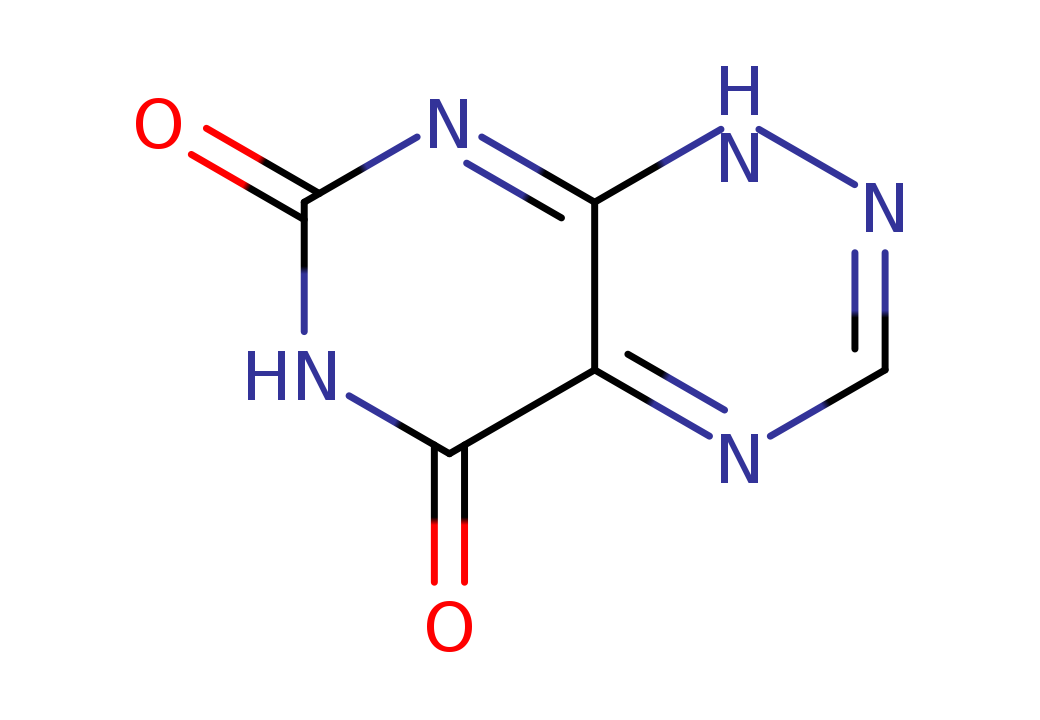
\includegraphics[align=t,width=0.25\textwidth]{data/badapple/medchem_01.png} & Scaffold of well-known toxin toxoflavin present in Burkholderia glumae, it was also previously identified by workers at Abbott using the ALARM NMR assay as a thiol trap and cause of false positives in HTS\cite{Huth2007-kc} \\
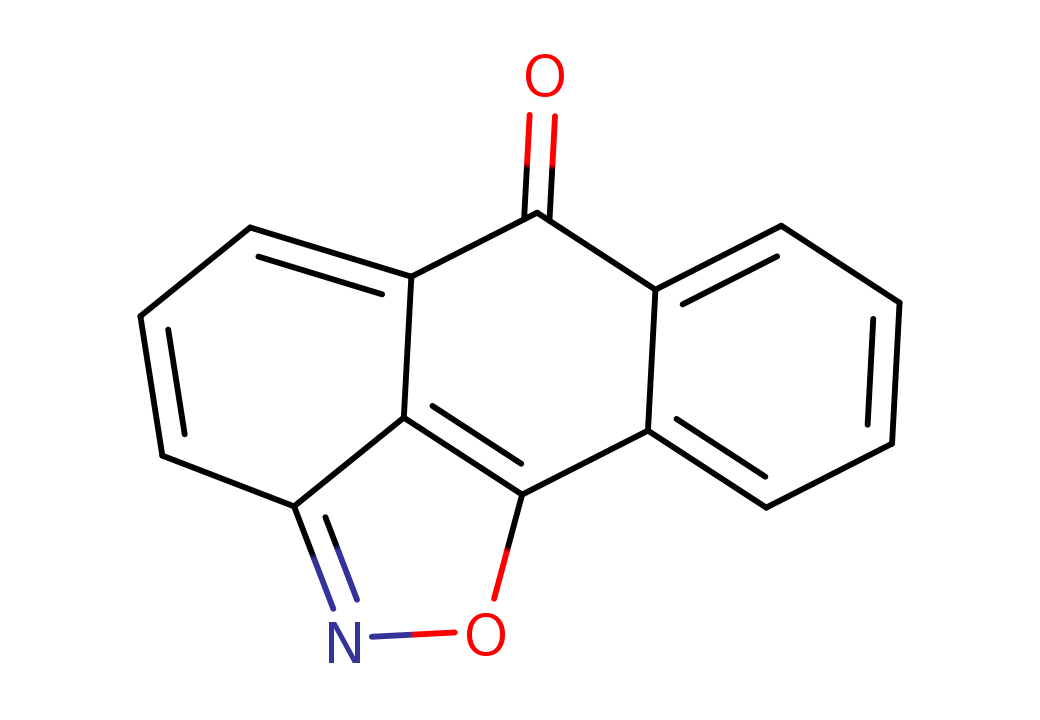
\includegraphics[align=t,width=0.25\textwidth]{data/badapple/medchem_02.png} & Scaffold a 6H-anthra[1,9-cd]isoxazol-6-one is known to react with DMSO acting as a nucleophile and undergoes N–O cleavage of the isoxazole ring to form the ring opened anthraquinone, a species known to form covalent adducts\cite{Sutter1982-qu} \\
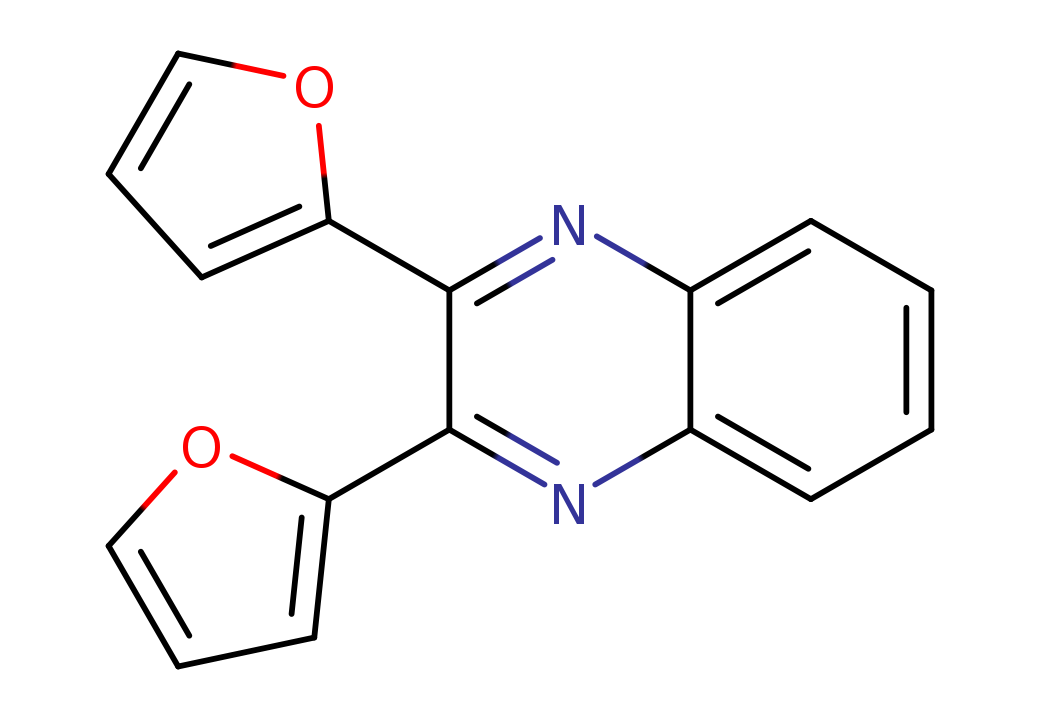
\includegraphics[align=t,width=0.25\textwidth]{data/badapple/medchem_03.png} & Scaffold likely made by reaction of orthophenylene diamine with the corresponding furanyl alpha diketone. It could be a false positive if contaminated with the furanyl alpha diketone. It has only weak metal coordinating activity \\
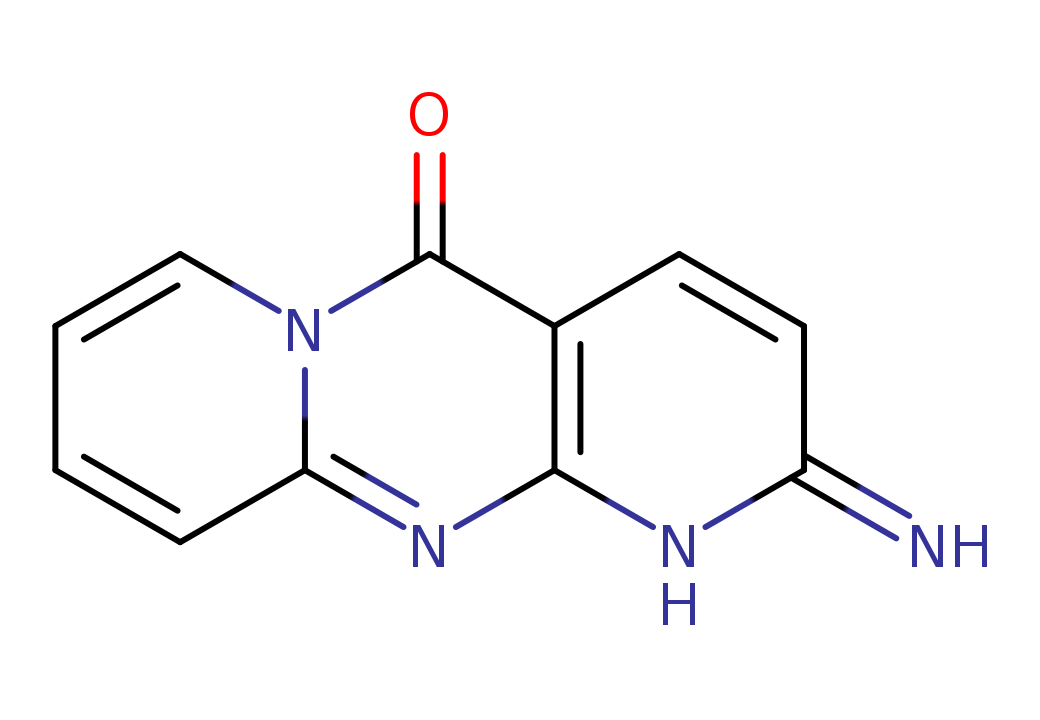
\includegraphics[align=t,width=0.25\textwidth]{data/badapple/medchem_04.png} & Scaffold the synthesis of the tricyclic scaffold by a malononitrile cyclization with a 2-amino-3-formyl-4-oxo-4H-pyrido[1,2-a] pyrimidine suggests that the
scaffold in this series may be susceptible to Michael attack at what was originally the formyl precursor carbon \\
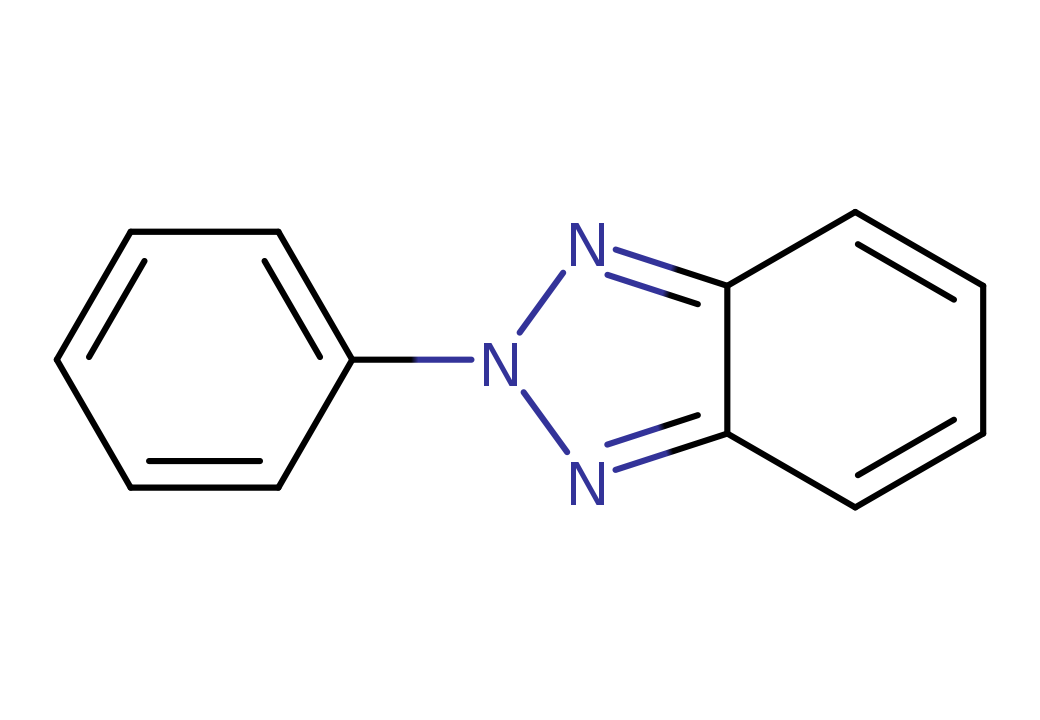
\includegraphics[align=t,width=0.25\textwidth]{data/badapple/medchem_05.png} & Scaffold is reported to possess strong fluorescence, UV absorbance as well as strong mutagenic activity\cite{Oda2008-at}. The phenyl-2-(2H-benzotriazol-2-yl) scaffold is also found in the photostabilizer Tinuvin P \\
\hline
\end{tabular}
\label{table:ba_cmp_medchem}
\end{table}

\begin{figure}
	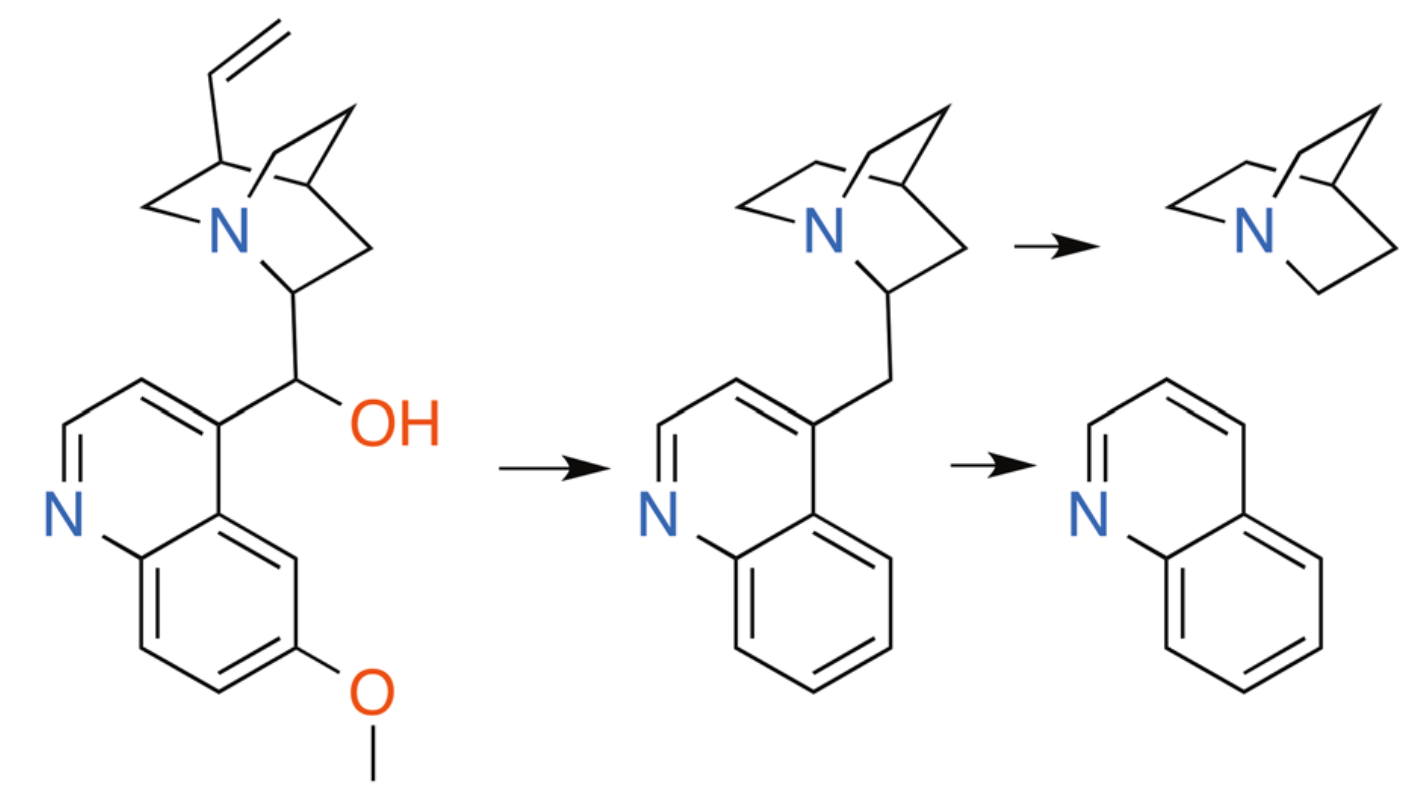
\includegraphics[width=\textwidth]{figures/badapple/Badapple_Fig5.png}
	\caption{HScaf scaffolds of quinine}
	\label{fig:BA_05}
\end{figure}

\subsection{PubChem assays and BARD experiments}

Badapple depends on the quantity and quality of input data, where quality includes both accuracy and semantic interpretability. In particular, it should be possible to rigorously resolve whether two assay results reflect the same or different bioactivity phenomena. This challenge has motivated several efforts to improve bioassay annotations, metadata and ontologies, including BAO and BARD. Badapple was designed to accommodate the uncertainties associated with the limited annotations of MLP assays in PubChem. However, it has been well understood that ontology improvements would offer new opportunities for Badapple and related extensions, for example, promiscuity assessment specific to a target class such as G-protein coupled receptors, and automatic extraction of privileged scaffolds from large scale screening data.

\subsection{Reconciling big data and small data}

Drug discovery campaigns rely on the expert judgment of medicinal chemists for key decisions on which leads to pursue. That expertise derives from formal training, project experience, and community knowledge which may be global or institutional. Cheminformatics and other areas have contributed tools to assist medicinal chemists, and Badapple is such a tool. As such, acceptance and effective use of Badapple will be enhanced if its advice is comprehensible and demonstrably consistent with expert medchem knowledge. To this end the medicinal chemist among us (CAL) evaluated and annotated top scoring scaffolds for chemical issues as drug leads, which are shown in table \ref{table:ba_cmp_medchem}, accompanied by relevant literature references\cite{Huth2007-kc,Sutter1982-qu,Oda2008-at}.

\begin{figure}
	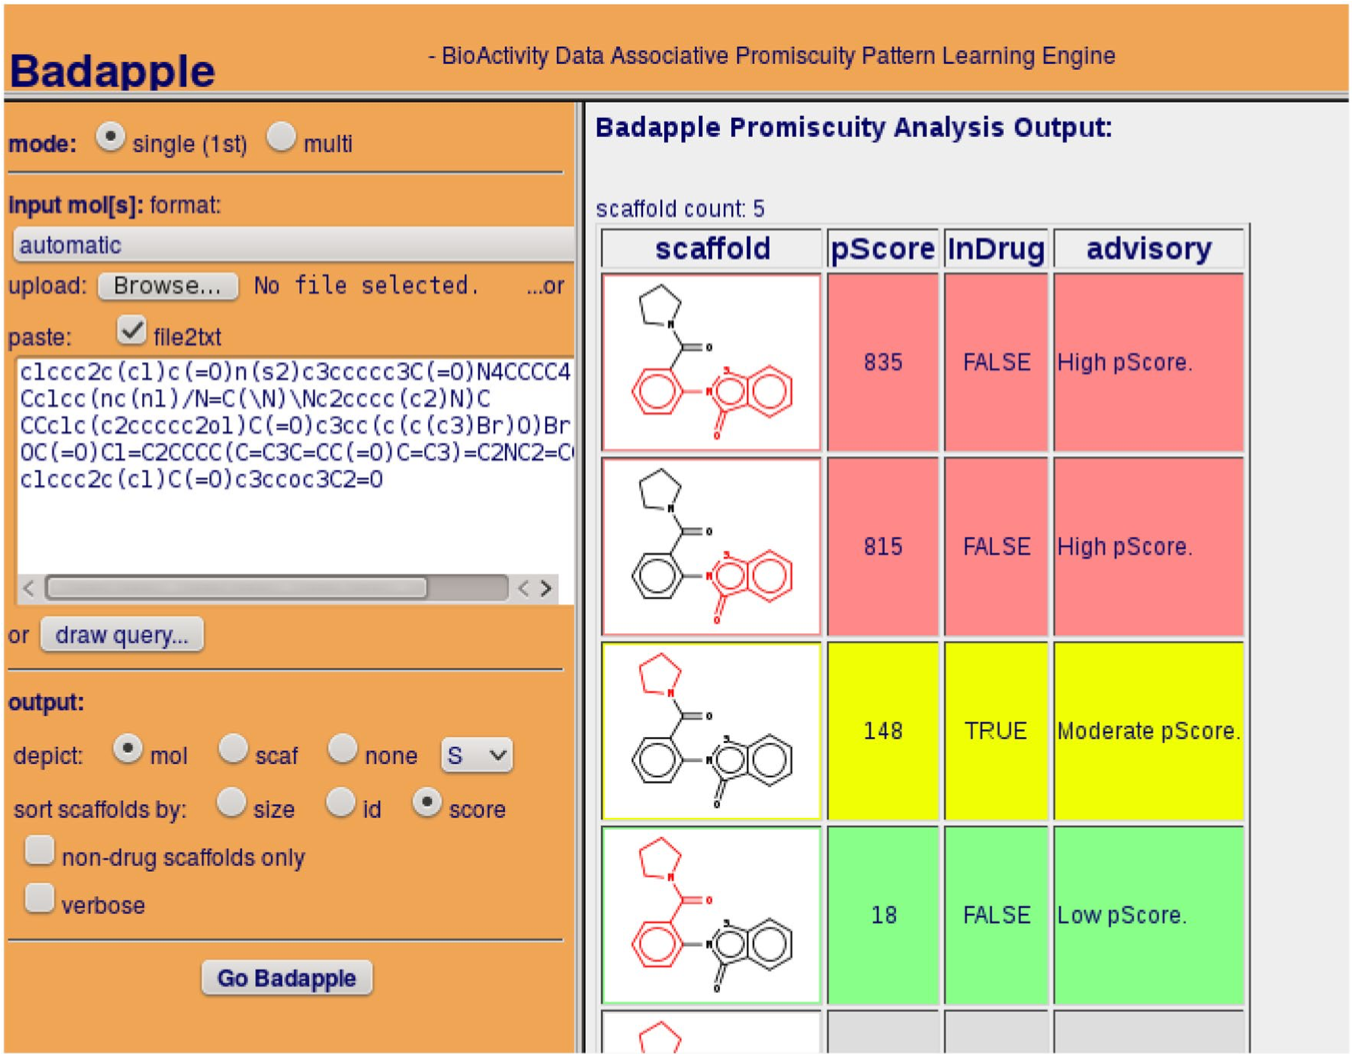
\includegraphics[width=\textwidth]{figures/badapple/Badapple_Fig6.png}
	\caption{Badapple public web app, available at https://datascience.unm.edu/public-biocomputing-apps}
	\label{fig:BA_06}
\end{figure}


\begin{figure}
	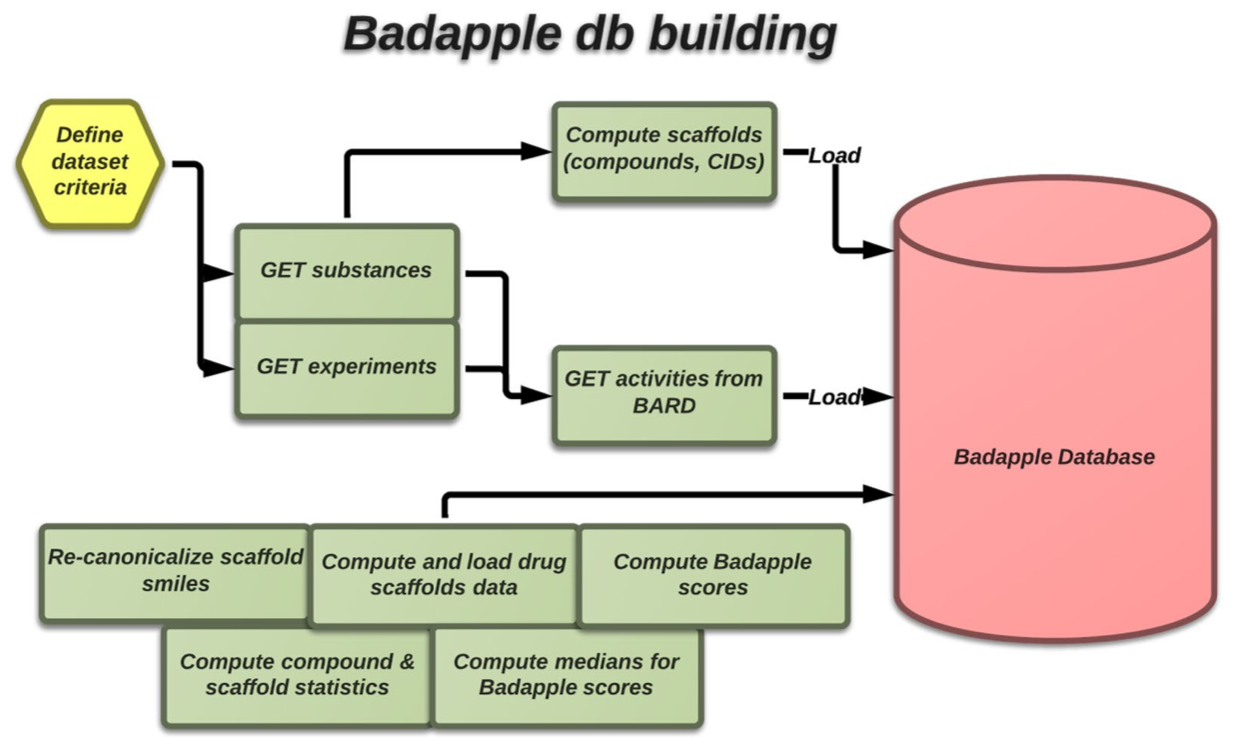
\includegraphics[width=\textwidth]{figures/badapple/Badapple_Fig7.png}
	\caption{Database workflow}
	\label{fig:BA_07}
\end{figure}

\section{Conclusions}

Badapple is an easy-to-use, readily interpretable algorithm and tool that can assist scientists in navigating a complex scientific and informational landscape. In particular, Badapple is designed for rapid detection of promiscuity patterns in HTS data, using public bioassay evidence. However, Badapple is designed to be trained with additional data, and to detect novel patterns, based on an entirely different chemical library. Compound promiscuity is generally undesirable but must be understood in light of polypharmacology and systems chemical biology. Badapple scores indicate either patterns of true or artefactual promiscuity, either of which can help guide an experimental research project away from “false trails”.

\section{Methods}

The Badapple datasets are all prepared from the MLSMR compound library and HTS bioassays involving at least 20K compounds, to optimize applicability to high-throughput screening methods. The “bard1” dataset was downloaded from BARD in January 2013 and is the default dataset for the analyses herein. BARD was in an early development phase at that time and the dataset is for all intents and purposes equivalent to a PubChem dataset. Accordingly, “bard1” is used in this paper to enhance reproducibility and comprehensibility. The “bard2” dataset was downloaded from BARD in June 2014, and includes fewer assays, reflecting the ongoing annotation and curation efforts at the time. For each dataset the compound library was filtered to remove any salt part and normalize charges. In total, the training data for Badapple was comprised of 389,533 compounds, 438,583 substances, 143,098 scaffolds, 822 HTS PubChem assays, and more than 220 million activity data. In these counts and workflows the terms “compound” and “substance” are defined as by PubChem: compounds as unique chemical structures, identified by CID, and substances as sourced and registered experimental materials, identified by SID. The HierS “hierarchical scaffold” algorithm was used to generate the scaffold library for all compounds. An illustration of the algorithm is shown in figure \ref{fig:BA_05}. The HierS algorithm perceives for any molecule a hierarchical set of scaffolds, the largest one being equivalent to the “Bemis–Murcko framework”\cite{Bemis1996-jg}, which consists of all ring-systems and linkers. Additional scaffolds represent all the combinations of ring-systems and linkers contained therein. Comprehensive output files and R code used for analysis are provided in supplemental materials (Additional file 2).

HierS and Badapple were implemented using the ChemAxon JChem Java toolkit\cite{ChemAxon2012-py} with both command line and web interfaces. The HierS implementation has been open-sourced\cite{Yang2012-qd}. Badapple is available as a public web app (see figure \ref{fig:BA_06}). See also supplementary figure of the Badapple plugin via BARD web client (Additional file 2).

A Badapple database was implemented with PostgreSQL, since rapid scoring, possibly for large numbers of compounds and scaffolds, requires pre-computing and storing aggregate statistics efficiently. OpenChord from gNova was used as a chemical cartridge. Scaffold analysis is performed for all compounds, resulting in links from scaffolds to compounds and substances. Activity data associates substances with an outcome for each sample (typically a well in a multiwell plate) in all the assays in the dataset. Typically there are hundreds of millions of samples. The workflow is outlined in figure \ref{fig:BA_07}. R was used for statistical analyses.

\section{Abbreviations}

\begin{table}
\caption{Abbreviations}
\begin{tabular*}{\linewidth}{@{\extracolsep{\fill}}rl}
\hline
\textbf{BA} & batting average \\
\hline
\textbf{BAO} & BioAssay Ontology \\
\hline
\textbf{BARD} & BioAssay Research Database \\
\hline
\textbf{HTS} & high-throughput screening \\
\hline
\textbf{ML} & machine learning \\
\hline
\textbf{MLP} & Molecular Libraries Program \\
\hline
\textbf{MLSMR} & Molecular Libraries Small Molecule Repository \\
\hline
\textbf{Ro5} & Rule of 5 \\
\hline
\textbf{SAR} & structure–activity relationships \\
\hline
\textbf{UNMCMD} & University of New Mexico Center for Molecular Discovery \\
\hline
\end{tabular*}
\end{table}

\section{Authors’ contributions}

CGB developed the scoring function and tested the method. JJY performed the data analysis and implemented the algorithm. CAL manually reviewed highly scored scaffolds. TIO conceptualized and coordinated the project, jointly with LAS. JJY, CGB, OU and TIO wrote and edited the manuscript. CAL and LAS reviewed the manuscript. All authors read and approved the final manuscript.


% Chapter: KGAP
\chapter{KGAP (Knowledge graph analytics platform combining LINCS and IDG for drug target illumination)}

\section{Introduction}

LINCS, "Library of Integrated Network-based Cellular Signatures", and IDG, "Illuminating the Druggable Genome", are both NIH projects and consortia that have generated rich datasets for the study of the molecular basis of human health and disease.  LINCS L1000 expression signatures provide unbiased systems/omics experimental evidence. IDG provides compiled and curated knowledge for illumination and prioritization of novel drug target hypotheses. Together, these resources can support a powerful new approach to identifying novel drug targets for complex diseases, such as Parkinson's disease (PD), which continues to inflict severe harm on human health, and resist traditional research approaches.

Integrating LINCS and IDG, we built the Knowledge Graph Analytics Platform (KGAP) to support an important use case: identification and prioritization of drug target hypotheses for associated diseases. The KGAP approach includes strong semantics interpretable by domain scientists and a robust, high performance implementation of a graph database and related analytical methods. Illustrating the value of our approach, we investigated results from queries relevant to PD. Approved PD drug indications from IDG’s resource DrugCentral were used as starting points for evidence paths exploring chemogenomic space via LINCS expression signatures for associated genes, evaluated as target hypotheses by integration with IDG. The KG-analytic scoring function was validated against a gold standard dataset of genes associated with PD as elucidated, published mechanism-of-action drug targets, also from DrugCentral. IDG's resource TIN-X was used to rank and filter KGAP results for novel PD targets, and one, SYNGR3 (Synaptogyrin-3), was manually investigated further as a case study and plausible new drug target for PD.

The synergy of LINCS and IDG, via KG methods, empowers graph analytics methods for the investigation of the molecular basis of complex diseases, and specifically for identification and prioritization of novel drug targets. The KGAP approach enables downstream applications via integration with resources similarly aligned with modern KG methodology. The generality of the approach indicates that KGAP is applicable to many disease areas, in addition to PD.

\subsection{Keywords}
Knowledge graph, graph analytics, systems biology, drug discovery, drug target, druggable genome, Parkinson's disease

\section{Background}

Integration of heterogeneous datasets is often essential for biomedical knowledge discovery, where relevant evidence may derive from diverse subdomains that include but aren't limited to: foundational biology, chemistry, clinical data, and social sciences of epidemiology and health economics. Furthermore, there is a need for judicious selection of data types and datasets to integrate, driven by scientific use cases, guided by applicability, accessibility, and veracity of datasets. Accordingly, we have integrated LINCS and IDG to identify and prioritize novel drug target hypotheses, via KG methods and tools. LINCS content includes assay results from cultured and primary human cells treated with bioactive compounds (small molecules or biologics) or genetic perturbations. IDG data utilized in this study include drug-disease associations, gene-disease associations and bibliometric scores from literature text mining.

Synergy of LINCS and IDG. LINCS and IDG are NIH Common Fund\cite{National_Institutes_of_Health_US_Department_of_Health_and_Human_Services_undated-jt} projects, chosen for integration for specific applicability to drug target discovery. LINCS, Library of Networked Cell-based Signatures, is described as a "System-Level Cataloging of Human Cells Response to Perturbations"\cite{Keenan2018-sf} and features experimental and computational methodology designed to generate useful biomedical knowledge from a systems/omics framework. As a key example, perturbagens (e.g., small molecules, ligands such as growth factors and cytokines, micro-environments, or CRISPR gene over-expression and knockdowns representing disease phenotypes) are characterized by proteomics, transcriptomics (RNA-seq), or biochemical and imaging readouts. Therefore LINCS provides useful mapping from genome to phenome with direct relevance to biomolecular mechanisms and therapeutic hypotheses. IDG\cite{Oprea2018-cp}, with its Target Central Resource Database (TCRD) and data portal Pharos\cite{Nguyen2017-lo}, integrates heterogeneous datasets from IDG experimental centers and diverse external sources with a clear purpose, to illuminate understudied ("dark") protein-coding genes as potential drug targets. IDG is particularly strong in text mining of current biomedical literature and bibliometrics suited for knowledge discovery and evidence evaluation, focused on the sciences of drug discovery research. In addition, another featured resource of IDG is DrugCentral\cite{Avram2021-wd}. DrugCentral provides information on active ingredients, chemical entities, pharmaceutical products, and their biological targets.

We have combined the complementary strengths of LINCS and IDG to derive new drug discovery insights via these synergies, particularly drug target hypotheses associated with diseases, phenotypes and cell lines. LINCS provides the comprehensive systems/omics view, while IDG focuses on relevant and robust evidence for drug target knowledge and validation. Table \ref{table:LINCS-IDG-Conc} summarizes key concepts and the semantic linkage of LINCS and IDG. Previously, LINCS studies have been designed to identify novel drug targets\cite{Chen2017-zj}, and IDG has included LINCS as a source for selected data\cite{Ursu2018-sc}. However, our approach provides a new KG method and platform to integrate and add value from these sources for an urgent and unmet scientific use case.

\begin{table}
\caption{Key concepts from LINCS and IDG}
\label{table:LINCS-IDG-Conc}
\begin{tabular}{|p{0.5\linewidth}|p{0.5\linewidth}|}
\hline
\makecell[c]{\textbf{LINCS key concepts}} & \makecell[c]{\textbf{IDG key concepts}} \\
\hline
\textbf{L1000}: Broad Institute microarray platform and LINCS project involving landmark genes. \newline
\textbf{Landmark Gene}: approximately 1000 genes representing the full human genome, from which a maximum set of gene responses can be inferred.\newline
\textbf{Cell Lines}: Primary cells and human patient induced pluripotent stem cells (iPSCs) representing diverse tissues and disease states (including ‘healthy’ controls).\newline
\textbf{Perturbagen}: A perturbagen may be chemical (drug-like), biologics, or genetic.\newline
\textbf{Signatures}: Various assays (transcriptomics, proteomics, or image analysis) are integrated together to identify patterns of common networks and cellular responses leading to predictive mechanistic interpretations.
& 
\textbf{Target}: Drug targets normally defined as human proteins or equivalently protein coding genes.\newline
\textbf{Mechanism of action}: Known, published, biochemical mechanism of pharmacological effect.\newline
\textbf{Disease}: Working definition is anything which could be the clinical indication for a drug.\newline
\textbf{Ligand}: Small molecule with known or hypothesized relationship with one or more targets.\newline
\textbf{Target Development Level (TDL)}: Simple measure of illumination: Tdark, Tbio, Tchem and Tclin.\newline
\textbf{Target Importance and Novelty}: Bibliometric measures from TIN-X for target prioritization. \\
\hline
\multicolumn{2}{|c|}{\textbf{LINCS-IDG semantic linkage}} \\
\hline
\multicolumn{2}{|p{1.0\linewidth}|}{LINCS centers utilize in-depth gene and protein expression assays to generate signatures directly mappable to IDG protein targets. Disease and phenotype ontology mapping is a community challenge with useful, working solutions such as UMLS\cite{Bodenreider2004-gn}. LINCS perturbagens include rigorously defined chemical entities and small molecule drugs included in IDG resource DrugCentral. Therefore, LINCS’s vast number of human cell lines and experimental chemical perturbation datasets, combined with IDG’s protein targets (gene and protein IDs) and DrugCentral active pharmaceutical ingredients (drug compounds) databases, provide a tightly integrated combination resource for drug target discovery.} \\
\hline
\end{tabular}
\end{table}


\begin{figure}
	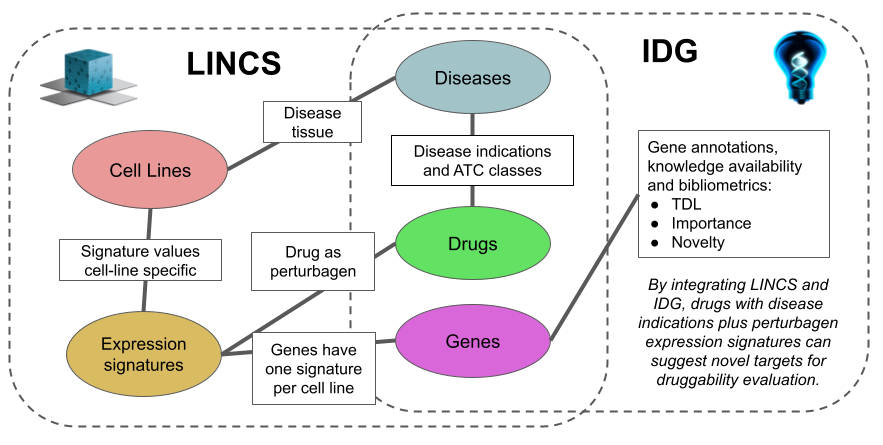
\includegraphics[width=\textwidth]{figures/kgap/KGAP_LINCS-IDG Schematic.png}
	\caption{Schematic of overall logic, that strong knowledge of approved drugs and cell lines associate diseases via LINCS expression signatures to differentially expressed genes, for IDG filtering and druggability evaluation.}
	\label{fig:KGAP_LINCS-IDG_Schematic}
\end{figure}

\section {Results}

\subsection{Graph analytics for evidence aggregation}

We used the list of PD drugs as starting points for evidence paths in KGAP to identify likely and novel PD targets. KGs and graph analytics provide an intuitive and powerful way to aggregate instances of evidence paths, yielding a score measuring the aggregated evidence. As illustrated schematically in figure \ref{fig:KGAP_LINCS-IDG_Schematic}, each evidence path connects a drug with expression signature and gene. The magnitude of the expression perturbation is represented by a z-score which can be used for thresholding and/or weighting. The search resulted in 641 genes, ranked by KGAP score produced by the graph analytics algorithm described in Methods and specified by Cypher query listing \ref{listing:kgap_01}.

\subsection{Validation versus known mechanism-of-action targets}

Solving the fundamental challenges of molecular biomedicine is an ongoing effort. Specifically, there are no gold standard validation datasets of causal or druggable genes for complex diseases, including cancers, neurodegenerative, metabolic, and cardiovascular diseases. Therefore it is pertinent to elucidate the genomic basis of diseases, and the fundamental uncertainties and difficulties concerning the definitions and diagnostic criteria for complex diseases such as PD. Mindful of these difficulties, we validated against a dataset of known drug targets, for the same PD drugs described above, all based on peer-reviewed references, and with elucidated mechanism-of-action (MoA), as manually curated in the DrugCentral database. Given the scientific and regulatory standards for efficacy met by approved drugs, and the standards of evidence for peer-reviewed, manually curated MoA targets, we consider this approach the most useful and informative dataset validation available. LINCS is experimental based, thus derived independently from the curation of MoA targets from DrugCentral, or in machine learning terms, there is strict separation of training and test data.

\begin{figure}[h]
\begin{subfigure}{0.5\textwidth}
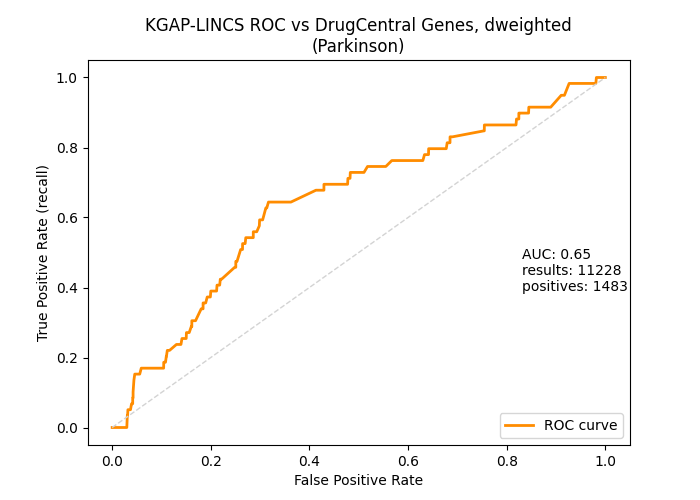
\includegraphics[width=0.95\linewidth]{figures/kgap/KGAP-LINCS_ROC_dweighted_Parkinson.png} 
\caption{}
\label{fig:KGAP-LINCS_ROCsa}
\end{subfigure}
\begin{subfigure}{0.5\textwidth}
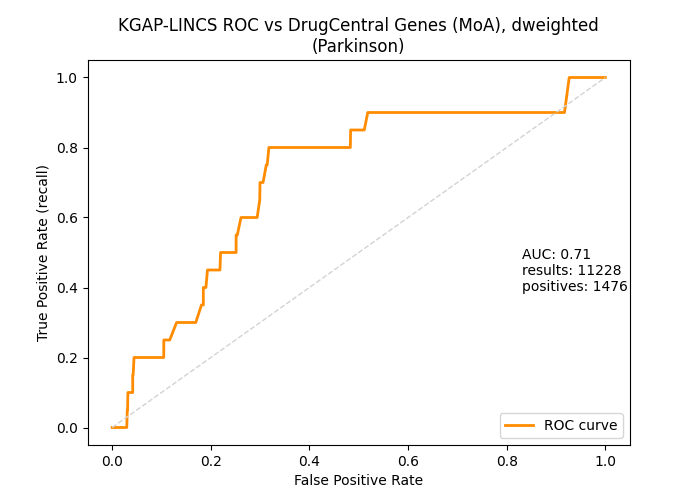
\includegraphics[width=0.95\linewidth]{figures/kgap/KGAP-LINCS_ROC_dweighted_MoA_Parkinson.png}
\caption{}
\label{fig:KGAP-LINCS_ROCsb}
\end{subfigure}

\begin{subfigure}{0.5\textwidth}
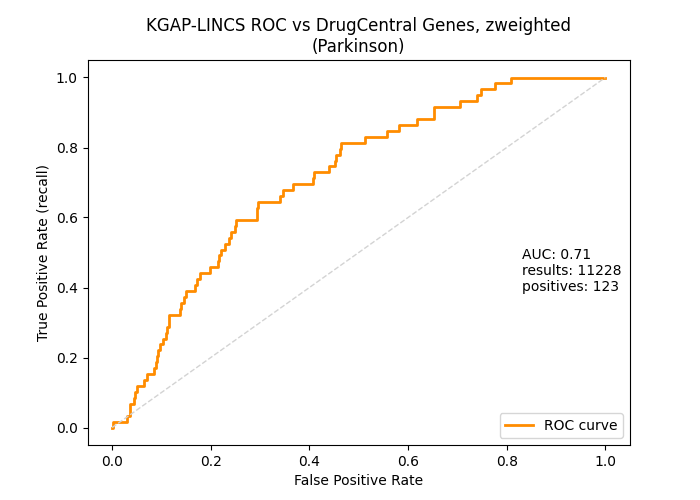
\includegraphics[width=0.95\linewidth]{figures/kgap/KGAP-LINCS_ROC_zweighted_Parkinson.png} 
\caption{}
\label{fig:KGAP-LINCS_ROCsc}
\end{subfigure}
\begin{subfigure}{0.5\textwidth}
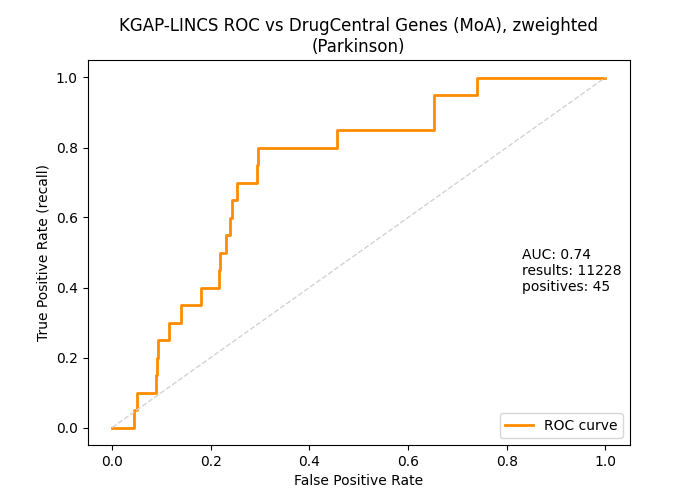
\includegraphics[width=0.95\linewidth]{figures/kgap/KGAP-LINCS_ROC_zweighted_MoA_Parkinson.png}
\caption{}
\label{fig:KGAP-LINCS_ROCsd}
\end{subfigure}

\caption{ROC curves with AUC for degree-only and z-score weighted evidence path graph analytics, validated against DrugCentral PD targets and known-with-MoA targets.}
\label{fig:KGAP-LINCS_ROCs}
\end{figure}

Figure \ref{fig:KGAP-LINCS_ROCs} shows validation receiver operating characteristic curve (ROC) plots for two variations of our method, and two validation sets. The "D-weighted" variation connotes weighting of evidence paths by the sum of degree at the LINCS expression signatures associating drugs and genes. The "Z-weighted" variation combines degree with the z-score expression level attribute associating signatures and genes. The two validation sets are (1) DrugCentral PD targets, and (2) DrugCentral PD targets with known MoA, as described above.  The ROC AUC (area under the curve) values range between 0.64 and 0.74, providing consistent, independent validation of the proposed method for disease to gene association discovery. The validation method, for PD or other disease queries, is reproducible using the source code repository referenced in the Availability of Data and Materials section. Note, the validation presented does not validate KGAP as a classification method. Evaluated as such, given the sparsity of known genes, the specificity is poor. However, classification is not the goal. Rather, our task is to aggregate and assess experimental evidence from LINCS which is applicable to PD as proof of concept. The validation presented simply measures overrepresentation, or enrichment, of known PD genes in relation to KGAP scores, indicating agreement and independent confirmation between two very different sources of knowledge, one purely experimental, the other expertly curated and peer-reviewed publication based. 

\subsection{Genes associated with PD, prioritized via IDG}

Gene hitlists generated by KGAP were mapped to druggability data from IDG. Target Development Level (TDL) provides a high-level classification into four groups — Tclin, Tchem, Tbio and Tdark — with respect to the depth of investigation from a clinical, chemical and biological standpoint. Further evaluation was explored via Target Importance and Novelty Explorer (TIN-X)\cite{Cannon2017-af}, an IDG project and bibliometric algorithm for evaluating disease-target associations from scientific literature. Moreover, TIN-X defines novelty as a bibliometric measure of occurrence rarity in the full PubMed corpus of titles and abstracts, and importance as a bibliometric measure of co-occurrence associating a specific disease and gene. The premise and motivation for IDG is that many understudied targets could offer new opportunities for medicines of novel therapeutic benefit. Hence TIN-X ranks and presents targets based on the principle of non-dominated solutions optimizing novelty and importance. nds\_rank=1 is assigned to all genes relative to which none are superior in both dimensions. nds\_rank=2 is this corresponding set with the first set removed, etc. In practice, typical users browse targets beginning at the outer boundary, using TDL color code as an additional guide. 

\begin{figure}[h]

\begin{subfigure}{1.0\textwidth}
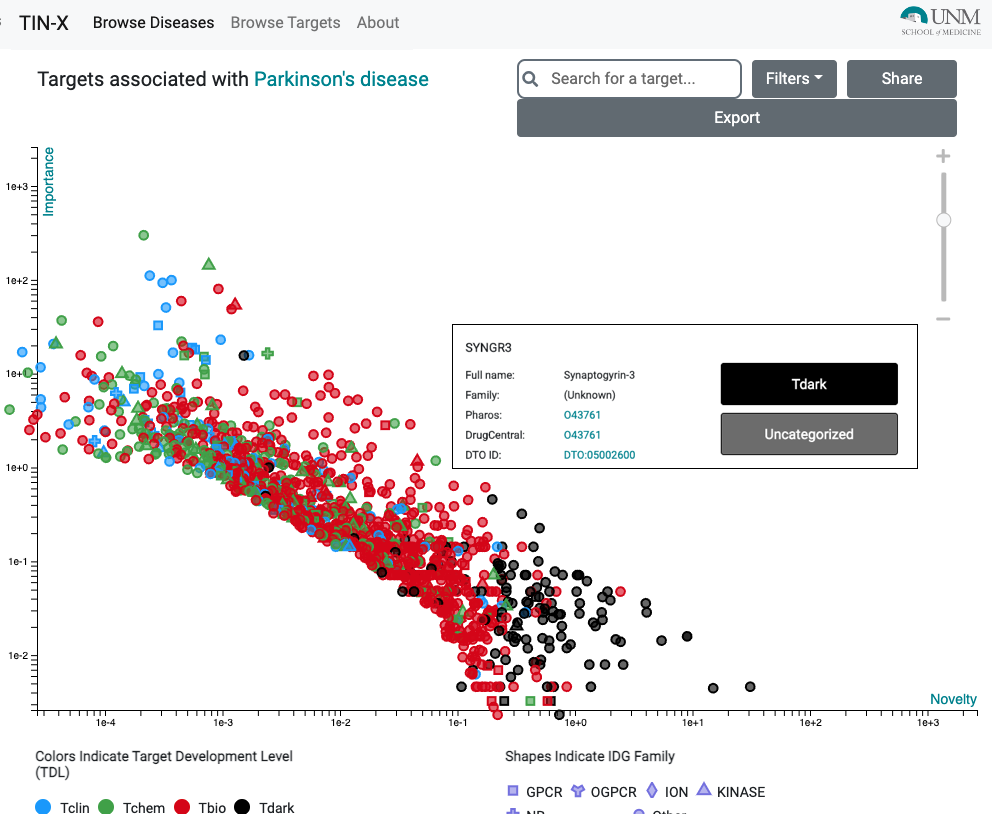
\includegraphics[width=0.95\linewidth]{figures/kgap/KGAP_TINX_SYNRG3_rev3.png} 
\caption{}
\label{fig:TINXa}
\end{subfigure}
\begin{subfigure}{1.0\textwidth}
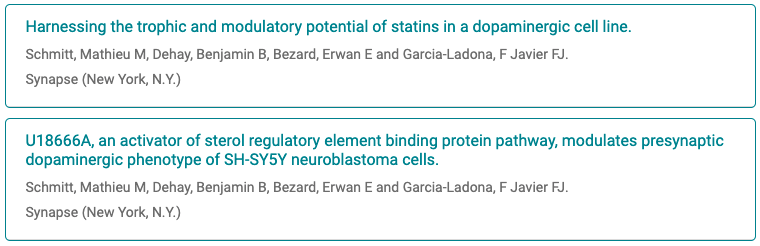
\includegraphics[width=0.95\linewidth]{figures/kgap/KGAP_TINX_SYNRG3articles_rev2.png}
\caption{}
\label{fig:TINXb}
\end{subfigure}

\caption{TIN-X scatterplot of genes for Parkinson's disease, DOID:14330, showing pop-up details for SYNGR3, Synaptogyrin-3, and publication details view for PD associated gene \emph{SYNGR3}.}
\label{fig:TINX}
\end{figure}

\subsection{Case study: \emph{SYNGR3}, Synaptogyrin-3}

To illustrate a typical use case, the KGAP hitlist was browsed for drug target illumination potential based on annotations from IDG. The highest ranked gene classified as Tdark is SYNGR3, Synaptogyrin-3. The exact function of SYNGR3 is unclear. However, recently a group provides evidence in the murine brain that SYNGR3 encodes for a synaptic vesicle protein that interacts with a dopamine transporter\cite{Egana2009-xo}. One of PD’s hallmark characterizations is the loss of nigrostriatal dopaminergic innervation\cite{Stoker2018-sf}. The high TIN-X rank (nds\_rank=6 out of 103) indicates both novelty and importance (PD-relevance), as shown in figure \ref{fig:TINXa}. Additionally, in figure \ref{fig:TINXb}, two reference publications present experimental and theoretical evidence for connection between statin drugs, therapeutic effectiveness for PD, and the gene \emph{SYNGR3}\cite{Schmitt2016-bf,Schmitt2017-du}. Figure \ref{fig:SYNGR3_subnet} displays evidence paths connecting SYNGR3 with associated expression signatures and drugs, matched by our method.

\begin{figure}
	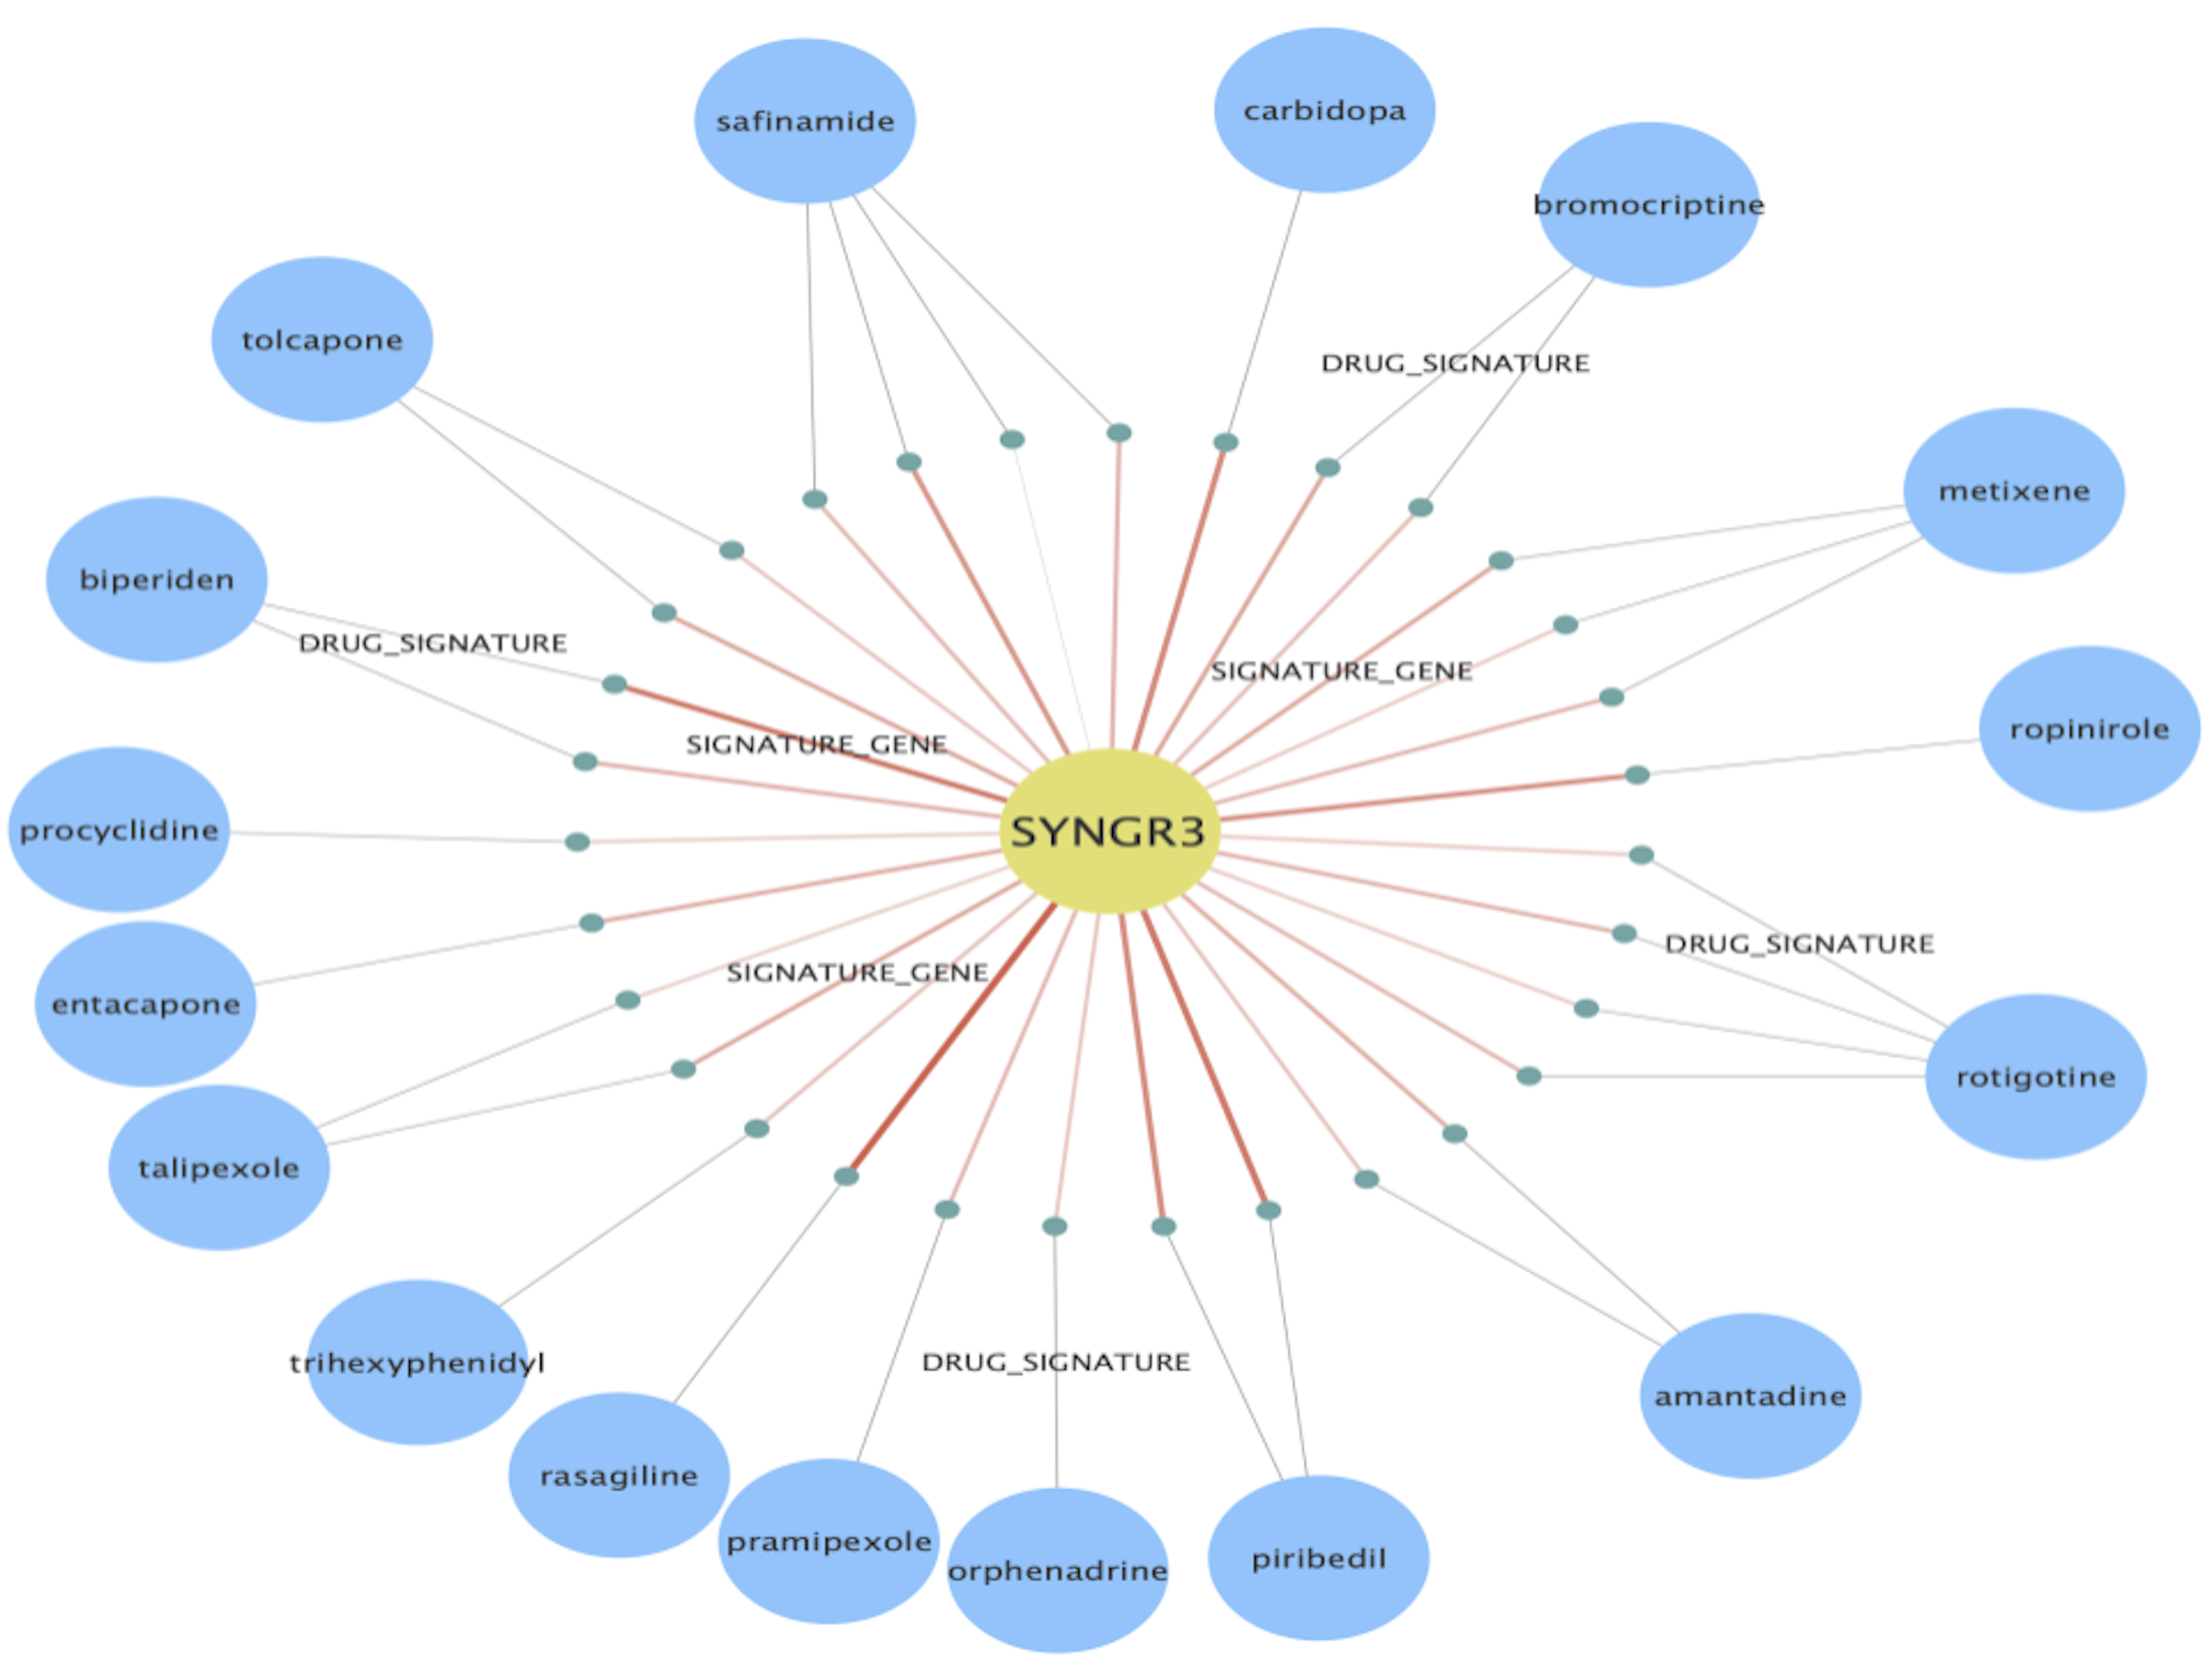
\includegraphics[width=\textwidth]{figures/kgap/KGAP_SYNGR3_subnet.png}
	\caption{Evidence paths generated from Cypher queries on our Neo4j graph database, for case study SYNGR3, showing associated expression signatures and drugs.}
	\label{fig:SYNGR3_subnet}
\end{figure}

\section{Discussion}

This project builds upon numerous prior efforts and resources, conceptual and technological, from domain specific data semantics, to graph database advances, conferring interoperability of depth and breadth\cite{Chen2010-to,Sirota2011-tl,Li2013-th,Callahan2013-ev,Himmelstein2015-ie,Greene2015-ix,Himmelstein2017-jy,Digles2018-qs,Szklarczyk2019-bc,Morton2019-le,Ochoa2020-ew}. The contributions cited relate and reflect a prodigious history of multidisciplinary community progress, spanning foundational biomedicine, computer science and informatics, from scientists collaborating effectively and rigorously via computational standards, tools and interfaces. Of particular relevance is the 2015 paper\cite{Himmelstein2015-ie} by Himmelstein and colleagues, as it employs a knowledge graph (KG) approach (termed Hetionet) applied to identifying disease-associated genes, closely related to drug target illumination. Other cited work is either not KG-based, or differing in application, and all lack the specificity of our approach both in terms of evidence sources and use-case focus. Another distinctive feature of our approach is its interpretability both algorithmically and in terms of provenance. For example, our validation performance (ROC AUC) is inferior but comparable to the performance reported by Himmelstein (e.g. .74 vs .79), but without training, which introduces knowledge bias, a concern in our domain where ground truth is commonly uncertain or incomplete. Our “machine learning-free” approach relies exclusively on significant LINCS expression signals (z-scores) combined with IDG for target illumination and prioritization. 

Regarding the now-common term knowledge graph (KG), there are variations of meaning, but we emphasize: (1) Knowledge with strong semantics via rigorous data modeling; (2) Graph analytics as powerful and intuitive tools for many biomedical applications and users\cite{Lysenko2016-ba}.  Hence, we use the term KG unambiguously and with specific commitments. Advances in KG technologies have empowered progress far beyond previous efforts. A case in point is Chem2Bio2RDF\cite{Chen2010-to,Chen2012-iq}, developed in the Wild Lab, enabled by RDF and SPARQL but limited for analytics applications by availability of high-performance triple-store technologies. Another project which one of us (JY) has co-developed is CARLSBAD\cite{Mathias2013-hj}, a bioactivity knowledge graph limited in analytics performance and versatility by its implementation as a relational database. Additional lessons learned relate to (1) Generality versus purposefulness, and (2) Volume versus veracity. Accordingly, this project has prioritized quality and simplicity to mitigate the common problems of (1) unfocused, incoherent interfaces, and (2) unreliable or noisy data. Interpretability also depends on understanding of the tool's purpose, logic, results, and their provenance and confidence. In many cases, simple and clearly focused tools enhance comprehensibility and usability. In contrast, a toolkit is multi-purpose. For this research the key aim is to find gene associations based on a disease or drug query.

Graph databases are one category of NoSQL (non-SQL or non-relational) databases which are designed to outperform relational databases for some specialized datasets and analyses, and are well suited for representing and exploring complex biological systems\cite{Himmelstein2015-ie,Have2013-hx,Yoon2017-jv}. Just as graph diagrams provide an intuitive way to represent and explore relationships between entities, graph databases leverage this intuition to provide both a physical storage method, and approach for combining diverse datasets for exploration and analysis. Neo4j was chosen as an exemplary leader among graph databases with a rich set of graph based capabilities (e.g. Graph Data Science library,  and libraries for accessing, flat files, databases, existing open standards such as SPARQL, and open standard in development GQL\cite{JCC_Consulting_Inc_acting_on_behalf_of_an_unincorporated_association_of_ISO_Graph_Query_Language_Proponents_and_licensed_under_the_Apache_License_Version_2_undated-lm}).  In addition, Neo4j offers a free, open source community edition\cite{Neo4j_Inc_undated-hy}, powerful and user-friendly desktop client, APIs, ample documentation, and a vibrant and supportive user community. Though the Neo4j product is featured prominently in this paper, it is important to note that alternative capable graph databases exist, such as DGraph\cite{Dgraph_Labs_Inc_undated-ko} and Amazon Neptune\cite{Amazon_Web_Services_Inc_undated-lu}. Moreover, Neo4j and other graph databases are built on the shoulders of many diverse contributors and strands of computer science, thus, Neo4j is featured as an exemplar for these advances, and a rational technology choice at this time for implementing our methods.

Development of this knowledge graph analytics platform (KGAP) with LINCS and IDG was motivated by use cases from IDG and its core purpose to illuminate understudied genes and new drug targets. Generally stated: For a given disease, what new drug targets are suggested by the evidence? LINCS data provides aggregated experimental evidence to establish a cell and expression signature based systems biology database, supporting rational aggregation of disease-gene associations, powered by KG analytics well suited both to path-based analytics and interpretation. Representing PD informatically is another key ingredient, addressed by clinical indications for approved drugs, knowledge meeting high regulatory standards. The definitions and nosology of PD and other complex diseases are critical issues and limitations relevant to this study and many others. Any hypotheses regarding PD presumes a useful definition, however biologically PD and its complexity are better described by subtypes and clinical phenotypes. Yet, extant data is generally organized by diseases and clinical diagnoses as historically developed.

\section{Conclusions}

A knowledge graph analytics platform (KGAP) was developed, integrating datasets from LINCS and IDG, for efficient search and aggregation of evidence paths based on a disease query, to identify, score and rank associated genes as drug target hypotheses. Approved indications for prescription drugs were used as high confidence entry points into the KG, and published MoA targets were used as a high confidence validation set. Modern graph database systems such as Neo4j provide a powerful suite of tools for high performance analytics, rigorously and reproducibly encoded, on semantically rich KGs, with interactivity and visualization enhancing human understanding. This study has demonstrated how KGAP can generate novel and plausible drug targets for Parkinson's disease. It includes a case study of the understudied "Tdark" SYNGR3 gene, scored highly by KGAP and supported independently by publications identified via the IDG application TIN-X. The KGAP approach and method as implemented is generalizable and applicable to drug target illumination in many other disease areas. Accordingly, in future work we intend to apply KGAP more broadly. 

\section{Methods}

\subsection{Data Sources}

As shown in figure \ref{fig:KGAP_LINCS-IDG_Schematic} an understanding of entities and the relationships between them can be quickly represented in a representative graph diagram, this establishes high level concepts and methods for discovering new insights, but also provides a clear design for the required extract transform and load (ETL) steps for building the capability.  The datasets listed here were used to construct a graph database instantiation of this design. From LINCS we used the L1000 Phase I and II Level 5 differential gene expression data, also termed the LINCS "Connectivity Map"\cite{Subramanian2017-sx}. Level 5 connotes the highest level of processing, normalization, evidence aggregation, and therefore confidence, interpretability, and interoperability. LINCS was processed using the same pipeline used by colleagues for the DrugCentral LINCS drug profiling tool, whereby differential gene expression data across 81 cell-lines were mapped to 1613 unique drug active pharmaceutical ingredients\cite{Avram2021-wd}.  Data and metadata files available from the LINCS Data Portal and NCBI Gene Expression Omnibus (GEO) were ETL-ed via 1.5TB PostgreSQL db. DrugCentral\cite{Avram2021-wd} (June 2020 version) was used for indications, ATC codes, chemical structures and other properties. IDG's TCRD, Target Central Resource Database\cite{IDG-KMC_Illuminating_the_Druggable_Genome_Knowledge_Management_Center_undated-pn}, (v6.7.0) provides gene properties including target development level (TDL: Tclin, Tchem, Tbio, Tdark) and gene family information.

\subsection{Data modeling, representing the knowledge}

Graphs in Neo4j are composed of nodes and relationships, which correspond with vertices and edges in graph theory terms, respectively. Graph queries can be thought of as patterns for matching paths through the graph, which consist of specified relationship types, each between two nodes, a semantic triple, subject-predicate-object. Neo4j is considered a schema-less database, meaning that data is loaded without constraints. But a strict schema with strong semantics informed by domain knowledge can be implemented, and is essential for accurate knowledge representation and interpretability. The meta-model for a graph can be reported by introspective Cypher query (CALL apoc.meta.graph). The meta-model for this graph is shown in figure \ref{fig:neo4jmetagraph}.


\begin{figure}
	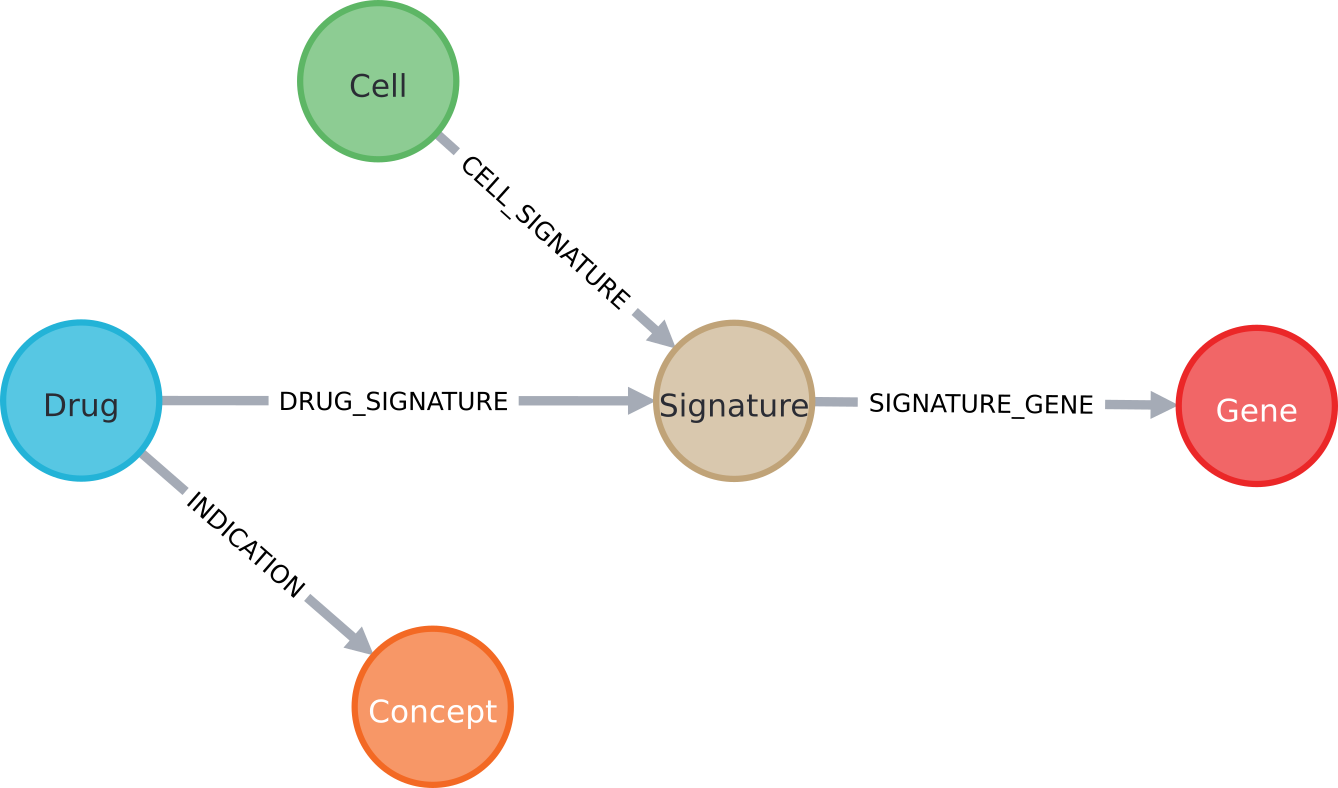
\includegraphics[width=\textwidth]{figures/kgap/KGAP_neo4jmetagraph.png}
	\caption{Neo4j meta graph. Both nodes and relationships have properties which can be used in query filtering and analysis.}
	\label{fig:neo4jmetagraph}
\end{figure}

Our graph is constructed of the following.

\textbf{Relationships}. INDICATION is constructed from DrugCentral indications  involving a Drug which is also a LINCS perturbagen. CELL\_SIGNATURE indicates the Cell type for the LINCS Signature. SIGNATURE\_GENE provides the differential expression z-score for the Gene. DRUG\_SIGNATURE associates the Drug involved for a given Signature.

\textbf{Nodes}. Concept consists of disease terms from DrugCentral with unique OMOP\cite{Hripcsak2019-ho} identifiers, and retaining other disease identifiers as properties for interoperability and extensibility. Drug nodes are derived by filtering for LINCS perturbagens which are in DrugCentral and have one or more indications.  Genes are from LINCS, with additional properties added from TCRD (e.g., development/druggability level). Cell and Signature nodes are from LINCS without filtering.

Table \ref{table:kg_rel} shows the complete list of relationships present in the graph and count, and table \ref{table:kg_node} the list of nodes with counts.

\begin{table}
\caption{Type of relationship, source, and total counts}
\begin{center}
\begin{tabular}{ |c|c|c|c|c| } 
\hline
\textbf{Vertex type} & \textbf{Edge type} & \textbf{Vertex type} & \textbf{Source} & \textbf{Count} \\ 
\hline
\textbf{Signature} & SIGNATURE\_GENE & Gene & L1000 & 45623637 \\ 
\hline
\textbf{Cell} & CELL\_SIGNATURE & Signature & L1000 & 591676 \\ 
\hline
\textbf{Drug} & DRUG\_SIGNATURE & Signature & L1000 & 85814 \\ 
\hline
\textbf{Drug} & INDICATION & Concept & DrugCentral, L1000 & 7164 \\ 
\hline
\end{tabular}
\end{center}
\label{table:kg_rel}
\end{table}

\begin{table}
\caption{Type of node, primary source/ source of additional properties, and total counts}
\begin{center}
\begin{tabular}{ |c|c|c| } 
\hline
\textbf{Vertex type} & \textbf{Source} & \textbf{Count} \\ 
\hline
Signature & L1000 & 591676 \\ 
\hline
Gene & L1000, TCRD & 12329 \\ 
\hline
Concept & DrugCentral 2021 & 2241 \\ 
\hline
Drug & L1000, DrugCentral 2021 & 1613 \\ 
\hline
Cell & L1000 & 99 \\ 
\hline
\end{tabular}
\end{center}
\label{table:kg_node}
\end{table}


We filter the 45.6M signature associations at z-score threshold $|z|>3$, to identify strong evidence and patterns, which results in 10,663,228 (d:Drug)--(s:Signature)--(g:Gene) paths. 

\subsection{Parkinson's disease drug-set}

To apply KGAP to PD knowledge discovery, the set of drugs indicated by PD and related conditions were identified using DrugCentral, which derives drug indication from FDA DailyMed (provides trustworthy information about marketed drugs in the United States), and maps SNOMED to OMOP terms\cite{Hripcsak2015-xo} for interoperability. A simple substring search for "Parkinson" matches five terms: "Parkinsonism", "Parkinson's disease", "Arteriosclerotic Parkinsonism", "Dementia associated with Parkinson's Disease", and "Neuroleptic-induced Parkinsonism." Requiring Anatomical and Therapeutic Classification (ATC) "nervous system" is intended to focus on the neurological etiology of PD rather than symptoms. This query returns 25 drugs, shown in table \ref{table:pd_drugset} with their PubChem CID, of which 22 / 25 are present in LINCS. This drug-set represents PD knowledge as in drug-set enrichment analysis (DSEA)\cite{Napolitano2016-ya}, analogous to gene-set enrichment analysis (GSEA).

\begin{table}
\caption{Drug-set representing Parkinson's disease, with DrugCentral and PubChem IDs}
\begin{center}
\begin{tabular}{ |l|c|c|c| } 
\hline
\textbf{Name} & \textbf{Struct\_ID} & \textbf{PubChem\_CID} & \textbf{In\_LINCS} \\
\hline
amantadine & 144 & 2130 & TRUE \\
\hline
apomorphine & 228 & 6005 & TRUE \\
\hline
benzatropine & 333 & 1201549 & TRUE \\
\hline
biperiden & 374 & 2381 & TRUE \\
\hline
bromocriptine & 403 & 31101 & TRUE \\
\hline
dexetimide & 831 & 30843 & FALSE \\
\hline
entacapone & 1018 & 5281081 & TRUE \\
\hline
levodopa & 1567 & 6047 & TRUE \\
\hline
melevodopa & 1673 & 23497 & FALSE \\
\hline
metixene & 1780 & 4167 & TRUE \\
\hline
opicapone & 5143 & 135565903 & FALSE \\
\hline
orphenadrine & 1999 & 4601 & TRUE \\
\hline
pergolide & 2105 & 47811 & TRUE \\
\hline
pimavanserin & 5142 & 10071196 & TRUE \\
\hline
piribedil & 2202 & 4850 & TRUE \\
\hline
pramipexole & 2233 & 119570 & TRUE \\
\hline
procyclidine & 2276 & 4919 & TRUE \\
\hline
rasagiline & 3521 & 3052776 & TRUE \\
\hline
rivastigmine & 2392 & 77991 & TRUE \\
\hline
ropinirole & 2402 & 5095 & TRUE \\
\hline
rotigotine & 2407 & 59227 & TRUE \\
\hline
safinamide & 4921 & 131682 & TRUE \\
\hline
selegiline & 2429 & 26757 & TRUE \\
\hline
tolcapone & 2697 & 4659569 & TRUE \\
\hline
trihexyphenidyl & 2745 & 5572 & TRUE \\
\hline
\end{tabular}
\end{center}
\label{table:pd_drugset}
\end{table}

\subsection{Graph analytics for evidence aggregation}

KGAP consists of the graph database described plus code and tools used to query the database for target associations from the input drug-set representing the disease of interest. In the current version of the platform, the queries were implemented via the Neo4j Python Driver\cite{Neo4j_Inc_undated-ly} and our prototype Python3 command-line applications and notebooks. As in the data modeling in the construction of the database, the Cypher graph queries must be crafted to accurately express the biomedical question, and justify useful interpretation of results. However, since the database was designed precisely for target association and ranking, the Cypher queries involved can be relatively terse. The query used to generate PD target associations is shown in listing \ref{listing:kgap_01}. The scoring function is responsible for aggregating evidence from signature counts and z-scores, to reflect that confidence increases with additional confirmatory data, and is an implementation of Stouffer's function, with all weights set to one (equation \ref{eq:kgap_stouffer}) for z-score meta-analysis, based on Fisher's function using p-values\cite{Rosenthal1978-in}. Though not used in KGAP for hypothesis testing, the reference indicates the function is well behaved and combines z-scores as intended. 

\begin{equation}
Z \sim \frac{\sum_{n=1}^{k}w_iZ_i}{\sqrt{\sum_{n=1}^{k}w_i^2}}
\label{eq:kgap_stouffer}
\end{equation}

Cypher query used for PD target association:\\
\rule[0.5ex]{\linewidth}{1pt}
\begin{singlespace}
\begin{lstlisting}[caption=KGAP Cypher query,label=listing:kgap_01]
MATCH p=(d:Drug)-[]-(s:Signature)-[r]-(g:Gene), p1=(s)-[]-(c:Cell)
WHERE (d.pubchem_cid in [2130, 2381, 4167, 4601, 4850, 4919, 5095, 
    5572, 6005, 6047, 23497, 26757, 30843, 31101,47811, 59227, 
    77991, 119570, 131682, 1201549, 1201549, 3052776, 4659569, 
    5281081, 10071196, 135565903])
WITH g, sum(r.zscore)/sqrt(count(r)) AS score
RETURN g.id, g.name, score
ORDER BY score DESC
\end{lstlisting}
\rule[0.5ex]{\linewidth}{1pt}
\end{singlespace}

\subsection{Executing the KGAP workflow}

In the current version, the workflow is executed via Python3 command-line application kgap\_analysis.py. Alternatively, the workflow may be executed via integrated development environment (IDE) such as PyCharm, as shown in figure \ref{fig:pycharm}. More details, including a Jupyter notebook KGAP workflow implementation, are available via the GitHub repository, \href{https://github.com/IUIDSL/kgap\_lincs-idg}{https://github.com/IUIDSL/kgap\_lincs-idg}. 

\begin{figure}
	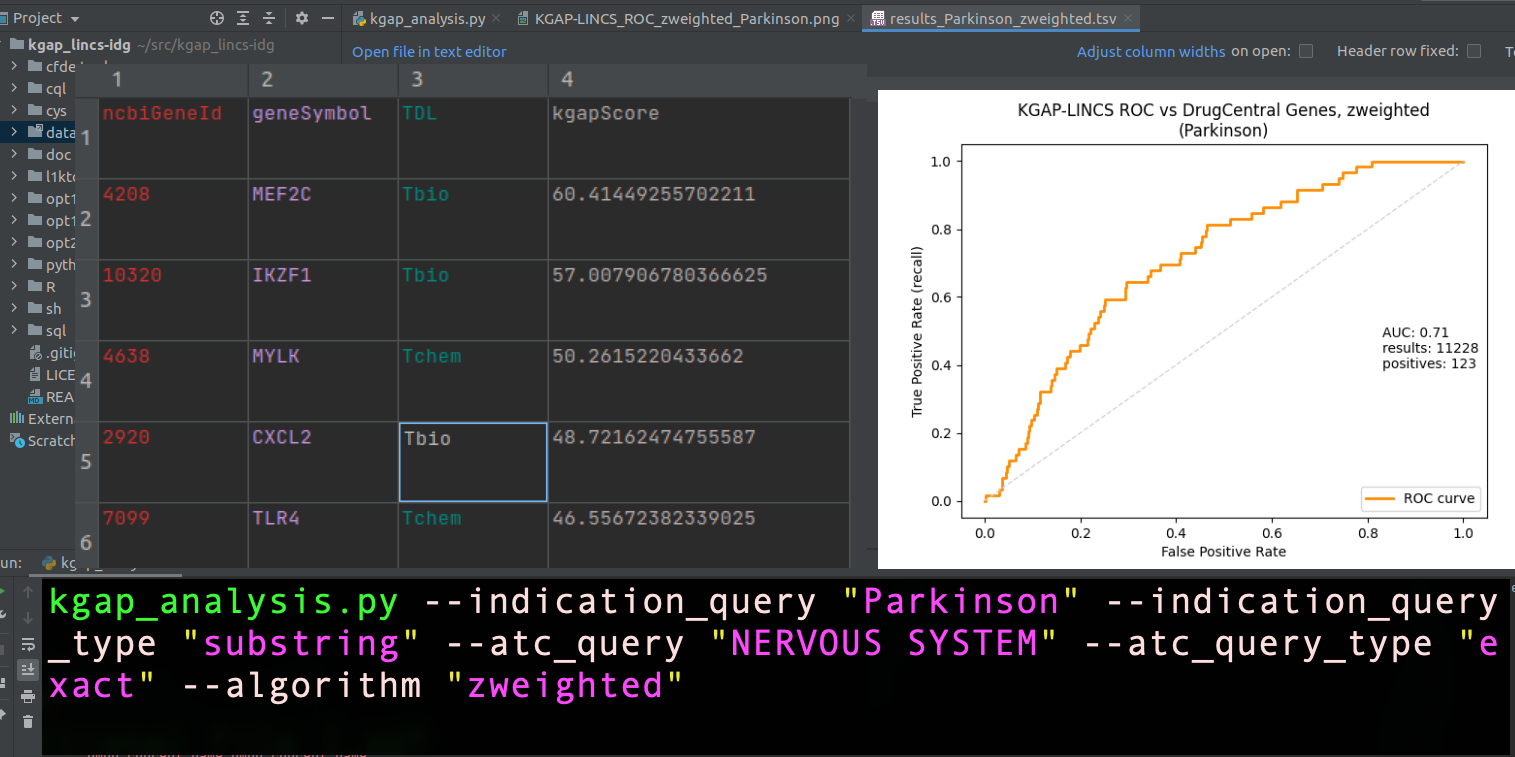
\includegraphics[width=\textwidth]{figures/kgap/KGAP_PyCharm_composite2.png}
	\caption{Composite image combining command line executing KGAP for "Parkinson",  output data table, and example ROC plot.}
	\label{fig:pycharm}
\end{figure}

\subsection{Exploring and visualizing the KG}

Human interaction with the KG through an effective GUI can greatly facilitate understanding and insights.  In this project we used (1) Neo4j Desktop, (2) Neo4j  Browser web client, used to produce Figure \ref{fig:neo4jmetagraph}, and (3) Cytoscape (v3.8.1) with the Neo4j plugin, which was used to produce figure \ref{fig:SYNGR3_subnet}.  

\section{Availability of data and materials}

Source code for processing and analysis is available publicly under Creative Commons Zero v1.0 Universal license at  \href{https://github.com/IUIDSL/kgap\_lincs-idg}{https://github.com/IUIDSL/kgap\_lincs-idg}. A Knime workflow is employed to extract, transform and load the graph database from sources, and generate TSV files of nodes and relationships. The database is queried, and results reported and visualized using Python and Cypher. A full dump of the KGAP\_LINCS-IDG dataset is available at \href{https://cheminfov.informatics.indiana.edu/projects/kgap/data/dclneodb.dump}{https://cheminfov.informatics.indiana.edu/projects/kgap/data/dclneodb.dump}. Source datasets used to build Neo4j database are: (1) DrugCentral-LINCS database dump: \href{https://cheminfov.informatics.indiana.edu/projects/kgap/data/drugcentral\_lincs.pgdump}{https://cheminfov.informatics.indiana.edu/projects/kgap/data/drugcentral\_lincs.pgdump}; (2) TCRD targets: \href{https://cheminfov.informatics.indiana.edu/projects/kgap/data/tcrd\_targets.tsv.gz}{https://cheminfov.informatics.indiana.edu/projects/kgap/data/tcrd\_targets.tsv.gz}. Neo4j Community Edition, Python, Scikit-learn, Cytoscape and other packages used in this work are freely and easily findable and accessible.

\section{Researcher contributions}

KGAP was an team science effort with several contributors. Joel Duerksen was lead developer for the Neo4j knowledge graph. Murat Ozturk was lead developer for the web UI LIDIA. Christopher Gessner was lead in graph analytics  and visualization methodology. Daniel Bieber contributed in application data science, and Jessica Binder in the biological case study of Synaptogyrin-3. JY was the overall scientific and informatics lead (\href{http://purl.org/spar/scoro/major-effort}{scoro:major-effort}), specifically:

\begin{itemize}
    \item Conceived and led research project (\href{http://purl.org/spar/scoro/conceives-project}{scoro:conceives-project}, \href{http://purl.org/spar/scoro/project-leader}{scoro:project-leader})
    \item Principal author of paper(\href{http://purl.org/spar/scoro/principal-author}{scoro:principal-author})
    \item Identified and sourced datasets from IDG and LINCS.
    \item Developed design for (1) knowledge graph, and (2) web UI
    \item Developed KGAP analysis and validation workflow via Cypher, Python and Jupyter. 
\end{itemize}




% Chapter: TIGA
\chapter{TIGA (Target illumination GWAS analytics)}

\textbf{Publication}: TIGA: Target illumination GWAS analytics, J. J. Yang et al., Bioinformatics, 2021\cite{Yang2021-di}.\\
\textbf{PI}: Tudor I Oprea, MD, PhD\\
\textbf{Web application}: \href{https://unmtid-shinyapps.net/tiga}{https://unmtid-shinyapps.net/tiga}\\
\textbf{Source code}: \href{https://github.com/unmtransinfo/tiga-gwas-explorer}{GitHub:tiga-gwas-explorer}\\
\textbf{Abbreviations}: Appendix \ref{appendix:tiga}

\section{Introduction}

Genome wide association studies (GWAS) can reveal important genotype–phenotype associations, however, data quality and interpretability issues must be addressed. For drug discovery scientists seeking to prioritize targets based on the available evidence, these issues go beyond the single study. Here, we describe rational ranking, filtering and interpretation of inferred gene–trait associations and data aggregation across studies by leveraging existing curation and harmonization efforts. Each gene–trait association is evaluated for confidence, with scores derived solely from aggregated statistics, linking a protein-coding gene and phenotype. We propose a method for assessing confidence in gene–trait associations from evidence aggregated across studies, including a bibliometric assessment of scientific consensus based on the iCite Relative Citation Ratio, and meanRank scores, to aggregate multivariate evidence. This method, intended for drug target hypothesis generation, scoring and ranking, has been implemented as an analytical pipeline, available as open source, with public datasets of results, and a web application designed for usability by drug discovery scientists, at https://unmtid-shinyapps.net/tiga/\cite{Yang2021-di}.

Over the two decades since the first draft human genome was published, dramatic progress has been achieved in foundational biology with translational benefits to medicine and human health. Genome wide association studies (GWAS) contribute to this progress by inferring associations between genomic variations and phenotypic traits\cite{Bosse2018-yl,Rusu2017-en}. These associations are correlations which may or may not be causal. While GWAS can reveal important genotype–phenotype associations, data quality and interpretability must be addressed\cite{Lambert2012-tr,Visscher2017-jp,Marigorta2018-xk,Gallagher2018-ev}.  For drug discovery scientists seeking to prioritize targets based on evidence from multiple studies, quality and interpretability issues are broader than for GWAS specialists. For this use case, GWAS are one of several evidence sources to be explored and considered, and interpretability must be in terms of genes corresponding to plausible targets, and traits corresponding to diseases of interest.

Single nucleotide variants (SNV) are the fundamental unit of genomic variation, and the term single nucleotide polymorphism (SNP) refers to SNVs identified as common sites of variation relative to a reference genome, and measured by microarray or sequencing technologies. The NHGRI-EBI GWAS Catalog\cite{Buniello2019-iw} -- hereafter "Catalog" -- curates associations between SNPs and traits from GWAS publications, shares metadata and summary data, standardizes heterogeneous submissions, maps formats and harmonizes content, mitigating widespread data and meta-data issues according to FAIR (Findable, Accessible, Interoperable and Reusable) principles\cite{Wilkinson2016-xu}. These challenges are exacerbated by rapid advances in experimental and computational methodology. As de facto GWAS registrar, the Catalog interacts directly with investigators and accepts submissions of summary statistic data in advance of publication. Proposing and maintaining metadata standards the Catalog advocates and advances FAIRness in GWAS, for the benefit of the community. The Catalog addresses many difficulties due to content and format heterogeneity, but there are continuing difficulties and limitations both from lack of reporting standards and the variability of experimental methodology and diagnostic criteria.

Other GWAS data collections include the Genome-Wide Repository of Associations between SNPs and Phenotypes, GRASP\cite{Eicher2015-ph} and The Framingham Heart Study, which employs non-standard phenotypes and some content from the Catalog (not updated since 2015). GWASdb\cite{Li2016-fo} integrates over 40 data sources in addition to the Catalog, includes less significant variants to address a variety of use cases, and has been maintained continually since 2011. GWAS Central, continually updated through 2019, includes less significant associations and provides tools for a variety of exploration modes based on Catalog data, but is not freely available for download. PheGenI\cite{Ramos2014-zq} integrates Catalog data with other NCBI datasets and tools. Others integrate GWAS with additional data (e.g. pathways, expression, linkage disequilibrium) to associate traits or diseases with genes\cite{Palleja2012-mb,Greene2015-ix,Shen2017-tt,Li2018-vj,Wainberg2019-ry}. Each of these resources offers unique value and features. For this use case, the Catalog is the logical choice, given its applicability and commitment to expert curation, data standards, support and maintenance.

Here we describe TIGA (Target Illumination GWAS Analytics), an application for illuminating understudied drug targets. TIGA enables ranking, filtering and interpretation of inferred gene-trait associations aggregated across studies from the Catalog. Each inferred gene-to-trait association is evaluated for confidence, with scores derived solely from evidence aggregated across studies, linking a phenotypic trait and protein-coding gene, mapped from single nucleotide polymorphism (SNP) variation. TIGA uses the Relative Citation Ratio, RCR\cite{Hutchins2016-hs}, a bibliometric statistic from iCite\cite{Hutchins2019-ue}. TIGA does not index the full corpus of GWAS associations, but focuses on the strongest associations at the protein-coding gene level instead, filtered by disease areas that are relevant to drug discovery. For instance, GWAS for highly polygenic traits are considered less likely to illuminate druggable genes. Here, we describe the web application and its interpretability for non-GWAS specialists. We discuss TIGA as an application of data science for scientific consensus and interpretability, including statistical and semantical challenges. Code and data are available under BSD-2-Clause license from https://github.com/unmtransinfo/tiga-gwas-explorer.

\subsection{Keywords}

GWAS, data science, drug discovery, drug target, druggable genome

\section{Methods}

\subsection{NHGRI-EBI GWAS Catalog preprocessing}

The 2021-02-12 release of the Catalog references 11671 studies and 4865 PubMed IDs. The curated associations include 8235 studies and 2706 EFO-mapped traits. After filtering studies to require (1) mapped trait, (2) p-value below 5e-8, (3) reported effect size (odds-ratio or beta), and (4) mapped protein-coding gene, we obtain 4118 studies, 1521 traits, and 10264 genes. For consistency between studies, only genes mapped by the Ensembl pipeline for genomics annotations were considered (not author-reported). Figures \ref{fig:TIGA_Study_coun} and \ref{fig:TIGA_Samp_sizes} illustrate the growth of GWAS research as measured by counts of studies and subjects.  

\begin{figure}
	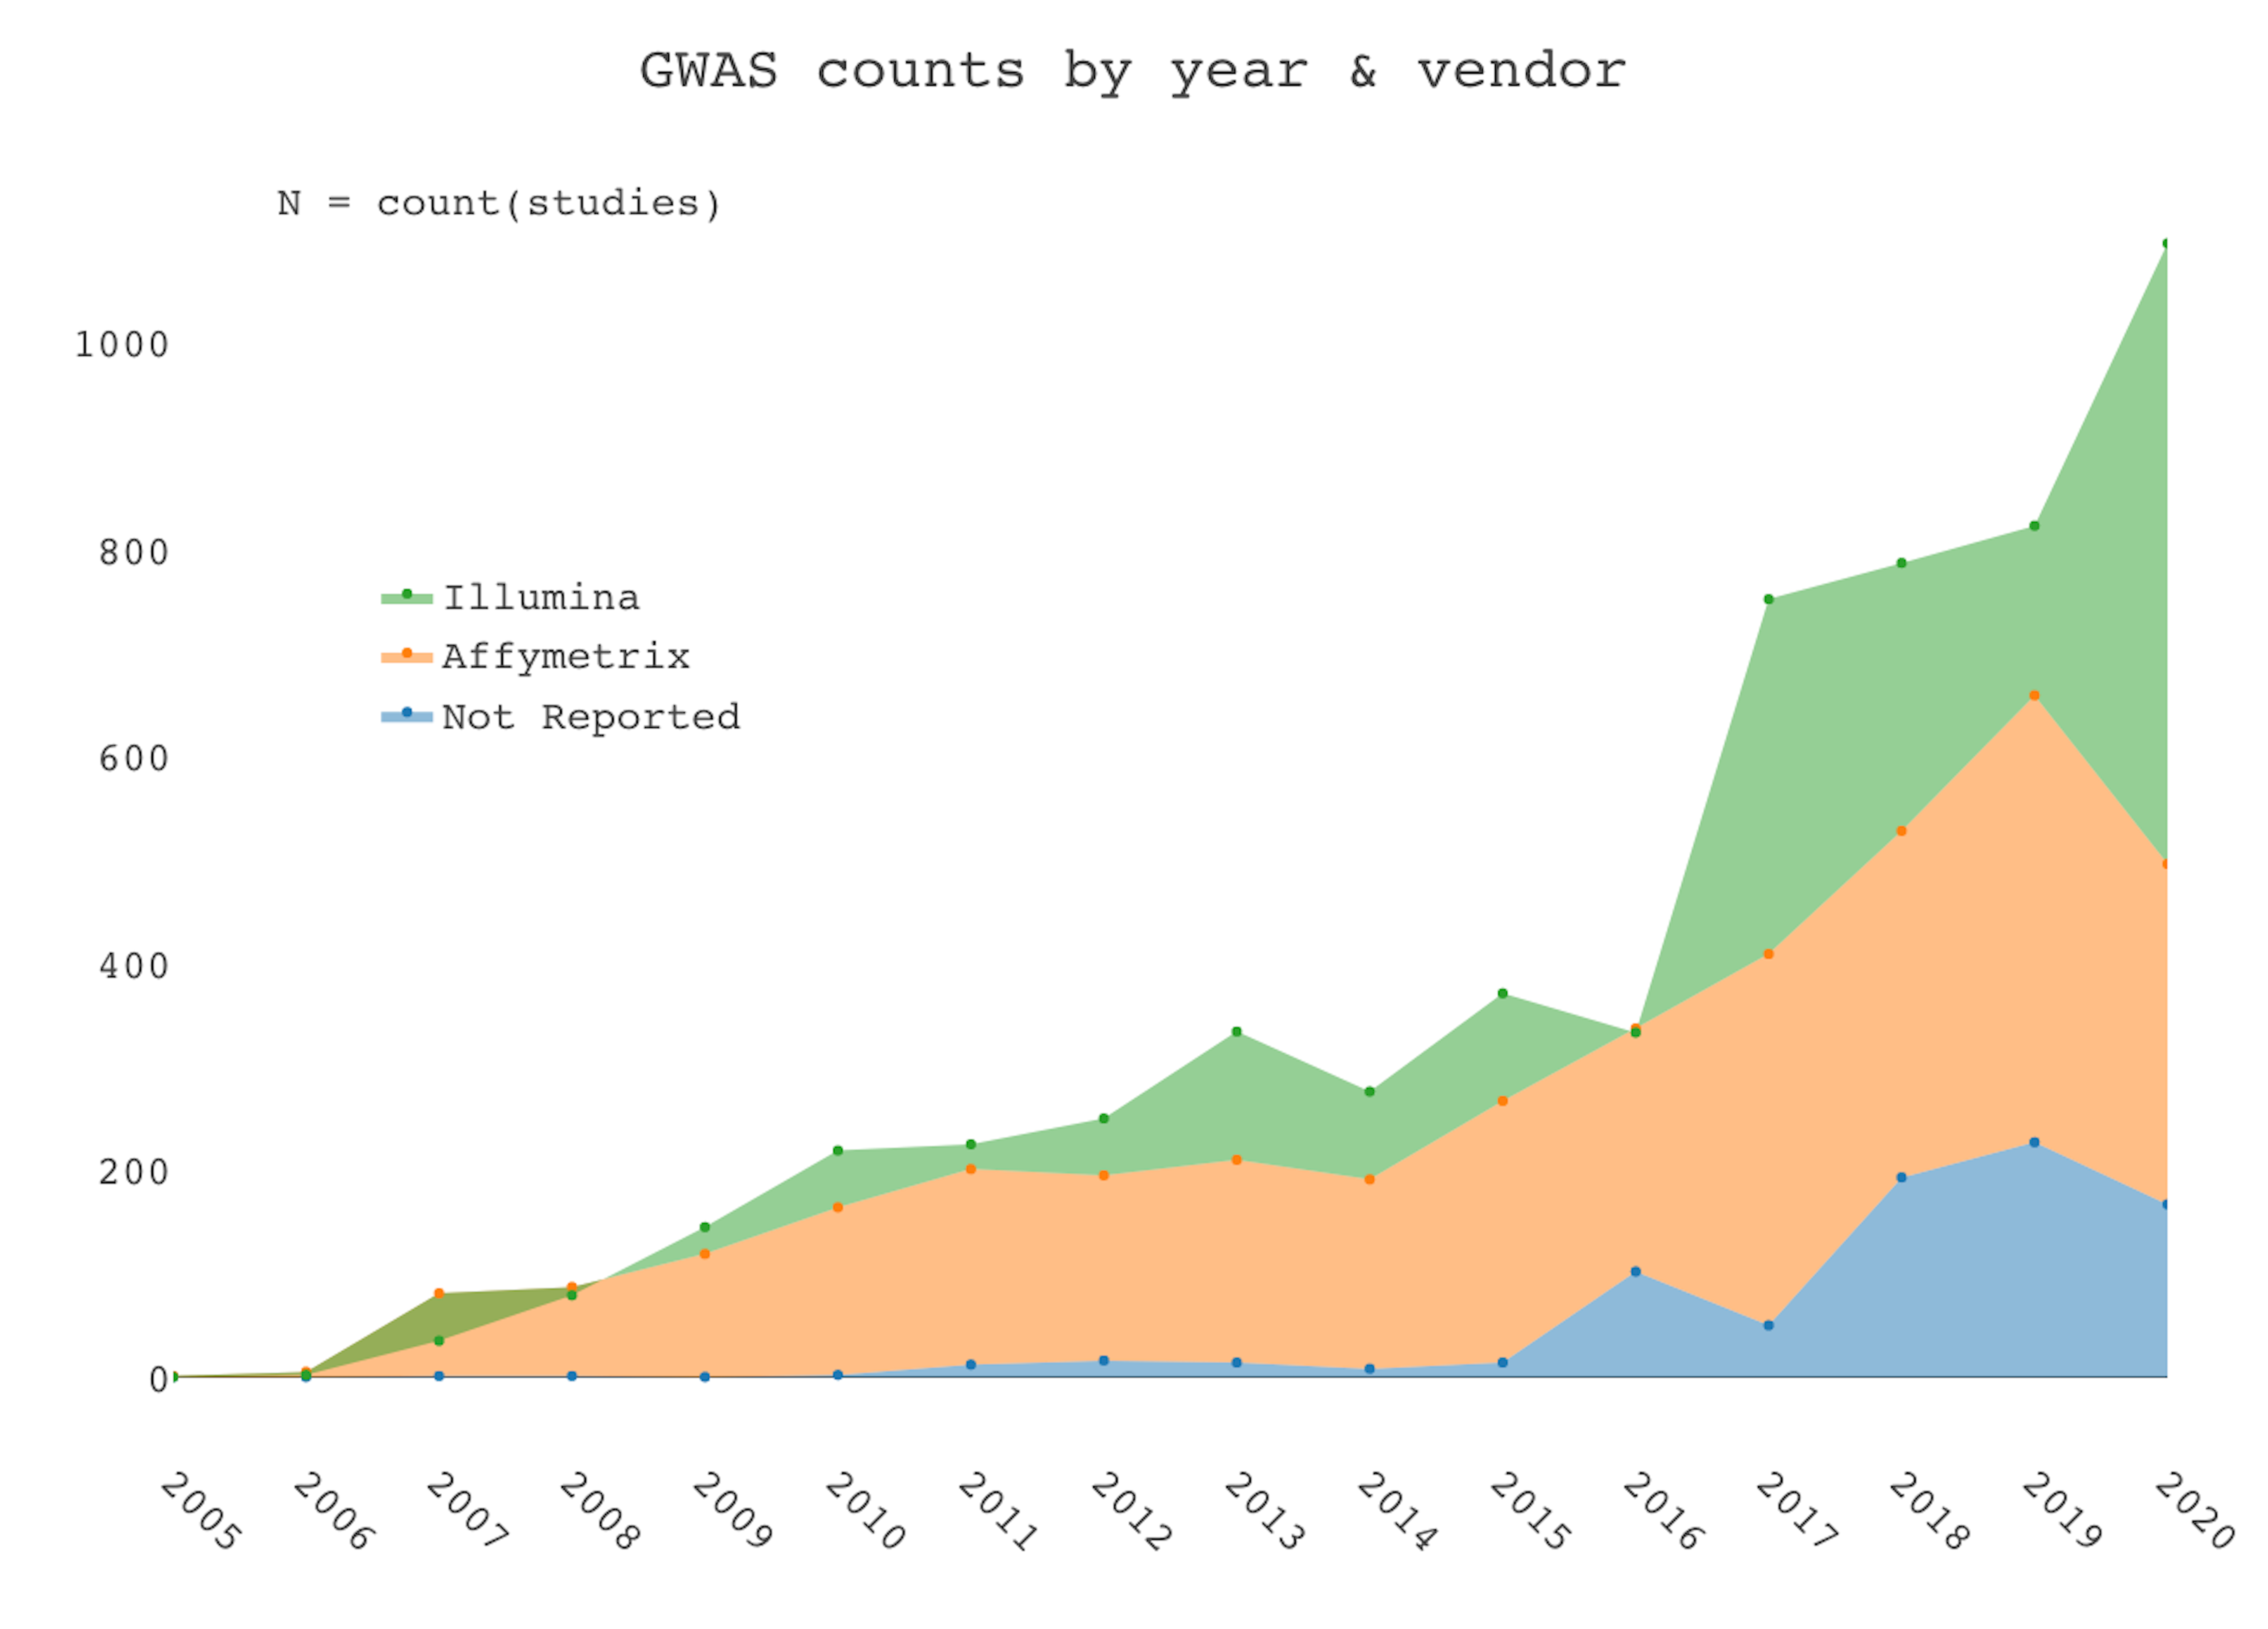
\includegraphics[width=\textwidth]{figures/tiga/FIG01_Study_counts.png}
	\caption{GWAS Catalog study counts by year and vendor, indicating growth and platform trends.}
	\label{fig:TIGA_Study_coun}
\end{figure}

\begin{figure}
	\includegraphics[width=\textwidth]{figures/tiga/FIG02_Sample_sizes.png}
	\caption{GWAS Catalog sample size distributions by year, on log scale, indicating variance in statistical power.}
	\label{fig:TIGA_Samp_sizes}
\end{figure}

\subsection{RCRAS = Relative Citation Ratio (RCR) Aggregated Score}

The purpose of TIGA is to evaluate the evidence for a gene-trait association, by aggregating multiple studies and their corresponding publications.  The iCite RCR\cite{Hutchins2016-hs} is a bibliometric statistic designed to evaluate the impact of an individual publication (in contrast to the journal impact factor).  By field- and time-normalizing per-publication citation counts, the RCR measures evolving impact, in effect a proxy for scientific consensus.  Hence by aggregating RCRs we seek a corresponding measure of scientific consensus for associations.

\begin{equation} RCRAS_{gt} = \sum_{study} \left(\frac{1}{gc} \sum_{pub} \frac{log_{2}(RCR + 1)}{sc}\right)
\end{equation}

Where\\
\begin{center}
\begin{tabular}{ r c l }
    $study$ & $=$ & GWAS (study\_accession)\\
	$gc$ & $=$ & gene count (in study)	\\
	$pub$ & $=$ & publication (PubMed ID)	\\
	$sc$ & $=$ & study count (in publication)	\\
\end{tabular}
\end{center}

The $log_2()$ function is used with the assertion that differences of evidence depend on relative, rather than absolute differences in RCR. Division by sc effects a partial count for publications associated with multiple studies.  Since $RCR \geq 0$, $log_2(RCR + 1) \geq 0$ and intuitively, when $RCR = 1$ and $sc = 1$, $log_2(RCR + 1) = 1$. Similarly division by gc reflects a partial count since studies may implicate multiple genes. This approach is informed by bibliometric methodology, including fractional counting, as described elsewhere [11]. For recent publications lacking RCR, we used the global median as an estimated prior. Computed thus, RCRAS extends RCR with similar logic, providing a rational bibliometric measure of evidence for scoring and ranking gene-trait associations. 

\subsection{Association weighting by SNP–gene distance}

Mapping  genomic  variation  of  single  nucleotides  (SNPs)  to  genes  is  a  challenging  area  of active  research\cite{Liu2010-fe,Mishra2015-rm,Lamparter2016-zb}.  This project  does not contribute to mapping methodology.  Rather, TIGA employs mappings provided by the Catalog between GWAS SNPs and genes,  generated by an Ensembl pipeline, which "adds additional SNP specific information associated with the rsID extracted... This information is retrieved using the Ensembl API and the source of the data is both Ensembl and NCBI."\cite{The_NHGRI-EBI_GWAS_Catalog_undated-kl} It is important to note that this method is unbiased and derived from experimental data and the current human reference genome . TIGA aggregates SNP-trait associations, assessing evidence for gene-trait associations, based on these understandings:

\begin{itemize}
\item SNPs within a gene are more strongly associated than SNPs upstream or downstream.
\item Strength of association decreases with distance, or more rigorously stated, the probability of linkage disequilibrium (LD) between a SNP and protein coding gene decreases with genomic physical distance. Accordingly, we employ an inverse exponential scoring function, consistent with LD measure ($\Delta$) and coefficient of decay ($B$) by Wang and coworkers\cite{Wang2006-ja}. 
\end{itemize}

This function (\ref{eq:TIGA_snpw}), used to weight N\_snp to compute a distance-weighted SNP count N\_snpw, is plotted together with the observed frequencies of mapped gene distances in supplementary figure \ref{fig:TIGA_Sup02}, to illustrate how the extant evidence is weighted. 

\begin{equation}
    N\_snpw = \sum_{i}^{N\_snp}  2^{-d_{i}/k}
    \label{eq:TIGA_snpw}
\end{equation}

\begin{center}
    where $ d = $ \emph{distance in base pairs}\\
    and $ k = $ \emph{"half-life distance"} (50k)
\end{center}

\begin{figure}
	\includegraphics[width=\textwidth]{figures/tiga/SupFIG02_distance_weighting_function.jpg}
	\caption{SNP-gene distances for (up|down)stream genes and TIGA weighting function}
	\label{fig:TIGA_Sup02}
\end{figure}

\subsection{Multivariate ranking}

Multivariate ranking is a well studied problem which needs to be addressed for ranking GWAS associations. We evaluated two approaches, namely non-parametric $\mu$ scores\cite{Wittkowski2008-mz} and meanRank, and chose the latter based on benchmark test performance. meanRank aggregates ranks instead of variables directly, avoiding the need for ad hoc parameters. Variable-ties imply rank-ties, with missing data ranked last. We normalize scoring to (0,100] defining meanRankScore as follows.

Variables of merit used for scoring and ranking gene-trait associations:

\begin{itemize}
\item N\_snpw: N\_snp weighted by distance inverse exponential described above.
\item pVal\_mLog: $max(-Log(pValue))$ supporting gene-trait association.
\item RCRAS: Relative Citation Ratio (RCR) Aggregated Score (iCite-RCR-based), described above.
\end{itemize}

Variables of merit and interest not currently used for ranking:

\begin{itemize}
\item OR: median(odds ratio, inverted if <1) supporting gene-trait association.
\item N\_beta: simple count of beta values with 95\% confidence intervals supporting gene-trait association.
\item N\_snp: SNPs involved with gene-trait association.
\item N\_study: studies supporting gene-trait association.
\item study\_N: mean(SAMPLE\_SIZE) supporting gene-trait association.
\item geneNtrait: total traits associated with the gene.
\item traitNgene: total genes associated with the trait.
\end{itemize}

N\_snp, N\_study, geneNtrait and traitNgene are counts of the corresponding unique entities. From the variables selected via benchmark testing the meanRankScore is computed thus:

\begin{equation}
    meanRankScore = 100 - Percentile(meanRank) = 100 - Percentile(\frac{1}{N} \sum_{i}^{N} rank_{i})
\end{equation}

\begin{center}
    where $ rank_{i} = $ \emph{rank of $ i $th variable}\\
    and $ N = $ \emph{number of variables considered}
\end{center}

$\mu$ scores were implemented via the muStat\cite{Wittkowski2012-fk} R package. Vectors of ordinal variables represent each case, and non-dominated solutions are cases which are not inferior to any other case at any variable. (For TIGA, cases are genes or traits, corresponding with trait-queries or gene-queries, respectively, and their variables of merit described above.) The set of all non-dominated solutions defines a Pareto-boundary. A $\mu$ score is defined simply as the number of lower cases minus the number of higher, but the ranking is the useful result. The ranking rule between case $k$ and case $k'$ may be formalized thus:

\begin{equation}
    \{ x_k < x_{k'} \} \Leftrightarrow \{ \forall_{l=1...L} x_{kl} \leq x_{k'l} \wedge \exists_{l=1...L} x_{kl} < x_{k'l} \}
\end{equation}


Simply put, case $k$’ is higher than case $k$ if it is higher in some variable(s) and lower in none.

\subsection{Validation: benchmark against gold standard}

Lacking a suitable gold standard set of gene–trait associations in general, we instead relied on established gene–disease associations from the Genetics Home Reference, GHR\cite{Fomous2006-wm} and UniProtKB\cite{UniProt_Consortium2018-kq} databases. This gold stand set was built following a previously described approach\cite{Pletscher-Frankild2015-oo}. It consists of 5,366 manually curated associations (positive examples) between 3,495 genes and 709 diseases. All other (2,472,589) possible pairings of these genes and diseases were considered negative examples.

To assess the quality of the TIGA gene–trait associations, we mapped the Ensembl gene IDs to STRING v11 identifiers using the STRING alias file\cite{Szklarczyk2019-bc} and the EFO terms to Disease Ontology\cite{Schriml2019-uh} identifiers based on ontology cross-references and the EMBL-EBI Ontology Xref Service. We then benchmark any individual-variable or multivariate ranking of the associations by constructing the receiver operating characteristic (ROC) curve by counting the agreement with the gold standard. See figure \ref{fig:TIGA_rocs}.

\section{Results}

\subsection{The TIGA web application}

\begin{figure}
	\includegraphics[width=\textwidth]{figures/tiga/FIG03_TIGA_EFO_0004612_plot.png}
	\caption{TIGA web application at https://unmtid-shinyapps.net/tiga/, displaying a plot of 644 genes currently associated with trait "high density lipoprotein cholesterol measurement" (EFO\_0004612).}
	\label{fig:TIGA_app}
\end{figure}

TIGA facilitates drug target illumination by currently scoring and ranking associations between protein-coding genes and GWAS traits. While not capturing the entire Catalog, the TIGA app can aggregate and filter GWAS findings for actionable intelligence, e.g., to enrich target prioritization via interactive plots and hitlists (figure \ref{fig:TIGA_app}), allowing users to identify the strongest associations supported by evidence.

Hits are ranked by meanRankScore described in Methods. Scatterplot axes are Effect (OR or N\_beta) vs. Evidence as measured by meanRankScore. Plot markers may be sized by pValue or RCRAS. This app accepts "trait" and "gene" query parameters via URL, e.g. ?trait=EFO\_0004541, ?gene=ENSG00000075073, ?trait=EFO\_0004541\&gene=ENSG00000075073.  Gene markers are colored by Target Development Level (TDL)\cite{Oprea2018-cp}. TDL is a knowledge-based classification that bins human proteins into four categories: Tclin, mechanism-of-action designated targets via which approved drugs act\cite{Santos2017-sd,Ursu2019-hx,Avram2020-ff}; Tchem are proteins known to bind small molecules with high potency; Tbio includes proteins that have Gene Ontology\cite{Ashburner2000-aw} “leaf” (lowest level) experimental terms; or meet two of these conditions:  A fractional publication count\cite{Pafilis2013-ml} above 5, three or more Gene “Reference Into Function” annotations\cite{Mitchell2003-ty}, or 50 or more commercial antibodies in Antibodypedia\cite{Bjorling2008-ia}; Tdark are manually curated UniProtKB proteins that fail to place in any of the previous categories.


\begin{figure}
\begin{subfigure}[c]{0.5\textwidth}
\includegraphics[width=8cm]{figures/tiga/FIG04_ROC_a.png}
\caption{Benchmark results against gold-standard disease–gene associations for the top-3 individual variables of merit.}
\label{fig:TIGA_rocs_a}
\end{subfigure}
\begin{subfigure}[c]{0.5\textwidth}
\includegraphics[width=8cm]{figures/tiga/FIG04_ROC_b.png}
\caption{Results for the multivariate ranking by meanRankScore and $\mu$ score.}
\label{fig:TIGA_rocs_b}
\end{subfigure}

\centering
\begin{subfigure}[c]{0.5\textwidth}
\includegraphics[width=\textwidth]{figures/tiga/SupFIG01_AdditionalROCs.png}
\caption{Benchmark for additional individual variables of merit not in the top 3.}
\label{fig:TIGA_Sup01}
\end{subfigure}
\caption{Performance evaluation. The performance of TIGA on the gold standard of gene-disease associations.}
\label{fig:TIGA_rocs}
\end{figure}

\subsection{Using TIGA for drug target illumination}

The main motivation of developing TIGA is to capture GWAS data when illuminating drug targets. Table \ref{table:idg_counts} shows how many targets from each protein family and IDG Target Development Level (TDL) are covered with associated traits in TIGA, with families as defined by Drug Target Ontology\cite{Lin2017-yb} (DTO) Level 2. IDG TDL is a knowledge based classification: Tclin = high-confidence drug targets; Tchem = small-molecule modulator exists; Tbio = biological function elucidated; Tdark = minimal knowledge\cite{Oprea2018-cp}. Coverage for the understudied 2,469 Tdark proteins is of particular interest. However, the data for other TDLs can also provide unique and complementary evidence, especially in case of Tbio proteins that are biologically characterized but have not before been clinically validated.


\begin{table}
\caption{TIGA mapped target (protein) counts by IDG Target Development Level (TDL) and Drug Target Ontology (DTO) level 2 gene family.}
\begin{center}
\begin{tabular}{ |l|c|c|c|c|c| } 
\multicolumn{1}{c}{} & \multicolumn{4}{|c|}{\textbf{Target Development Level (TDL)}} &  \multicolumn{1}{c}{}\\
\hline
\makecell[c]{\textbf{Family}} & \textbf{Tclin} & \textbf{Tchem} & \textbf{Tbio} & \textbf{Tdark} & \textbf{Total}\\
\hline
GPCR & 73 / 101 & 78 / 143 & 73 / 129 & 110 / 407 & 334 / 780\\
Ion channel & 97 / 127 & 59 / 89 & 72 / 116 & 12 / 20 & 240 / 352\\
Kinase & 57 / 66 & 278 / 360 & 97 / 133 & 12 / 20 & 444 / 579\\
Calcium-binding  & 3 / 5 & 1 / 3 & 58 / 93 & 8 / 11 & 70 / 112\\
Cell-cell junction & 0 / 0 & 0 / 0 & 22 / 49 & 8 / 12 & 30 / 61\\
Cell adhesion & 0 / 1 & 0 / 2 & 23 / 52 & 6 / 15 & 29 / 70\\
Cellular structure & 4 / 10 & 5 / 11 & 244 / 323 & 44 / 86 & 297 / 430\\
Chaperone & 0 / 1 & 8 / 9 & 27 / 46 & 6 / 8 & 41 / 64\\
Enzyme modulator & 4 / 5 & 25 / 44 & 376 / 532 & 50 / 101 & 455 / 682\\
Enzyme & 69 / 104 & 277 / 387 & 1022 / 1553 & 177 / 332 & 1545 / 2376\\
Epigenetic regulator & 9 / 13 & 41 / 55 & 16 / 22 & 0 / 1 & 66 / 91\\
Extracellular & 0 / 1 & 0 / 1 & 50 / 57 & 8 / 9 & 58 / 68\\
Immune response & 0 / 1 & 0 / 2 & 13 / 41 & 4 / 6 & 17 / 50\\
Nuclear rec & 16 / 18 & 16 / 19 & 8 / 11 & 0 / 0 & 40 / 48\\
Nucleic acid binding & 0 / 1 & 13 / 19 & 354 / 603 & 67 / 131 & 434 / 754\\
Transcription factor & 1 / 2 & 12 / 16 & 385 / 557 & 73 / 163 & 471 / 738\\
Transporter & 31 / 37 & 63 / 82 & 405 / 605 & 105 / 160 & 604 / 884\\
Receptor & 20 / 24 & 6 / 12 & 157 / 225 & 27 / 55 & 210 / 316\\
Signaling & 13 / 24 & 24 / 32 & 245 / 338 & 17 / 34 & 299 / 428\\
Storage & 0 / 1 & 0 / 1 & 2 / 7 & 1 / 2 & 3 / 11\\
Surfactant & 0 / 0 & 0 / 0 & 3 / 5 & 0 / 0 & 3 / 5\\
Other & 95 / 134 & 233 / 337 & 3973 / 6131 & 1734 / 3416 & 6035 / 10018\\
\hline
Total & 492 / 676 & 1139 / 1624 & 7625 / 11628 & 2469 / 4989 & 11725 / 18917\\
\hline
\end{tabular}
\end{center}
\label{table:idg_counts}
\end{table}

\begin{figure}
	\includegraphics[width=\textwidth]{figures/tiga/FIG05_EFO_0004612_hitlist.png}
	\caption{Examples of understudied genes for trait "high density lipoprotein cholesterol measurement" in TIGA.}
	\label{fig:TIGA_05}
\end{figure}


\begin{figure}
	\includegraphics[width=\textwidth]{figures/tiga/FIG06_EFO_0004612-GIMAP6_provenance.png}
	\caption{Provenance for association between gene GIMAP6 “GTPase IMAP family member 6” and trait "high density lipoprotein cholesterol measurement".}
	\label{fig:TIGA_06}
\end{figure}


Figures \ref{fig:TIGA_app} and \ref{fig:TIGA_05} illustrate a typical use case, the plot and gene list for trait "high density lipoprotein cholesterol measurement", which monitors blood levels of high density lipoprotein cholesterol as a risk factor for heart disease. Figure \ref{fig:TIGA_06} shows the provenance for one of the associated genes, GIMAP6 “GTPase IMAP family member 6” with the scores and studies for this gene-trait association, including links to the Catalog and PubMed. GIMAP6 is an understudied (Tbio) member of the GTPases of immunity-associated protein family (GIMAP). Although literature-based evidence of its potential role in cholesterol homeostasis is scarce\cite{Hoffmann2018-yh,Richardson2020-re}, this finding is substantiated by significantly increased circulating HDL cholesterol levels in GIMAP6-knock-out female mice [https://bit.ly/3uznvCU], suggesting that loss of GIMAP6 function may be associated with hypercholesterolemia-associated disorders.

\begin{figure}
	\includegraphics[width=\textwidth]{figures/tiga/FIG07_ EFO_0004541_Plot.png}
	\caption{TIGA web application at https://unmtid-shinyapps.net/tiga/, displaying a plot of genes associated with trait "HbA1c measurement" (EFO\_0004541).}
	\label{fig:TIGA_07}
\end{figure}

\begin{figure}
	\includegraphics[width=\textwidth]{figures/tiga/FIG08_EFO_0004541-SLC25A44_provenance.png}
	\caption{Provenance for association between gene SLC25A44 "Solute carrier family 25 member 44" and trait "HbA1c measurement".}
	\label{fig:TIGA_08}
\end{figure}

Figures \ref{fig:TIGA_07} and \ref{fig:TIGA_08} illustrate another target illumination example, for trait "HbA1c measurement" (glycated hemoglobin, signifying prolonged hyperglycemia), highly relevant to the management of type 2 diabetes mellitus\cite{Rahbar1969-vx,Saudek2009-bi}. Figure \ref{fig:TIGA_08} shows the provenance for one of the associated genes, SLC25A44 "Solute carrier family 25 member 44" with the scores and studies for this gene-trait association, including links to the Catalog and PubMed. SLC25A44 is an understudied (Tdark) branched-chain amino acid (BCAA) transporter that acts as metabolic filter in brown adipose tissue, contributing to metabolic health\cite{Yoneshiro2019-ke}. SLC25A44 may be involved in subcutaneous white adipose BCAA uptake and catabolism\cite{Lee2021-re}. 

\section{Discussion}

\subsection{Target illumination}

The explicit goal of the NIH Illuminating the Druggable Genome (IDG) program\cite{Oprea2018-cp} is to "map the knowledge gaps around proteins encoded by the human genome." TIGA is fully aligned with this goal, as it evaluates the GWAS evidence for disease (trait) – gene associations. TIGA generates GWAS-centric trait–gene association dataset using an automated, sustainable workflow amenable for integration into the Pharos portal\cite{Nguyen2017-lo,Sheils2021-ft}. The Open Targets platform\cite{Ochoa2020-ew,Ghoussaini2021-au} uses Catalog data and other sources, assisted by supervised machine learning, to identify probable causal genes, and validate therapeutic targets by aggregating and scoring disease–gene associations for "practicing biological scientists in the pharmaceutical industry and in academia." Open Targets associations are enhanced, but also limited, by the training data and knowledge sources reflecting current understandings of genetics. In contrast, TIGA provides aggregated evidence solely from the Catalog, reflecting experimental results with minimal or no bias, thus more interpretable in terms of provenance and methodology, and more suitable for some downstream consumers and use cases.

\subsection{From information to useful knowledge}

In data-intensive fields such as genomics, specialized tools facilitate knowledge discovery, yet interpretation and integration can be problematic for non-specialists. Accordingly, this unmet need for integration and interpretation requires certain layers of abstraction and aggregation, which depend on specific use cases and objectives. Our target audience is drug discovery scientists for whom the aggregated findings of GWAS, appropriately interpreted, can provide additional value as they seek to prioritize targets. This clear purpose serves to focus and simplify all aspects of its design. Our approach for evidence aggregation is simple, easily comprehensible, and based on what may be regarded as axiomatic in science and rational inductive learning: First and foremost, evidence is measured by counting independent confirmatory results.

Interpretability concerns exist throughout science, but GWAS is understood to present particular challenges\cite{Lambert2012-tr,Visscher2017-jp,Marigorta2018-xk,Gallagher2018-ev}. The main premise of GWAS is that genotype-phenotype correlations reveal underlying molecular mechanisms. While correlation does not imply causation, it contributes to plausibility of causation.  Genomic dataset size adds difficulty.  The standard GWAS p-value significance threshold is 5e-8, based on overall p-value 0.05 and Bonferroni multiple testing adjustment for 1-10 million tests/SNPs\cite{Marigorta2018-xk}. The statistical interpretation is that the family-wise error rate (FWER), or overall probability of a type-1 error, is 5\%, but associations to mapped genes require additional interpretation. Motivated by, and despite these difficulties, it is our belief that GWAS data can be rationally interpreted and used by non-specialists, if suitably aggregated. Accordingly, TIGA is a rational way to suggest and rank research hypotheses, with the caveat that the identified signals may be accompanied by experimental noise and systematic uncertainty.

\begin{figure}
	\includegraphics[width=\textwidth]{figures/tiga/FIG09_TIGA_Workflow.jpg}
	\caption{TIGA data sources and interfaces. TIGA integrates GWAS data from the Catalog and several other sources to rank gene-disease associations. These associations can be accessed through the TIGA webapp and are integrated into the DISEASES\cite{Pletscher-Frankild2015-oo} and Pharos platforms. Bulk download is also available.}
	\label{fig:TIGA_09}
\end{figure}

\subsection{Designing for downstream integration}

Biomedical knowledge discovery depends on integration of sources and data types which are heterogeneous in the extreme, reflecting the underlying complexity of biomedical science. These challenges are increasingly understood and addressed by improving data science methodology. However, provenance, interpretability and confidence aspects are underappreciated. As in all signal propagation, errors and uncertainty accrue and confidence decays. Here, we proposed the use of simple, transparent, and comprehensible metrics to assess the relative confidence of disease-gene associations, via the unbiased meanRank scores. Figure \ref{fig:TIGA_09}, summarizing TIGA sources and interfaces, illustrates its well-defined role. Continuous confidence scores support algorithmic weighting and filtering. Standard identifiers and semantics support rigorous integration. Limiting provenance to the Catalog and its linked publications, semantic interpretability is enhanced. TIGA was designed an implemented with downstream integration and interpretability in mind, and has been integrated with DISEASES and Pharos. TIGA is similarly well suited for KG integration, with well defined semantics for traits, genes, and SNPs.

\section{Conclusions}

We agree with Visscher et al. that: "the paradigm of 'one gene, one function, one trait' is the wrong way to view genetic variation"\cite{Visscher2017-jp}. Yet given the intrinsic complexity of biomedical science, progress often requires simplifying assumptions. Findings must be interpreted in context for an audience and application. Mindful of these concerns and limitations, TIGA provides a directly interpretable window into GWAS data, specifically for drug target hypothesis generation and elucidation. As interest in "interpretable machine learning" and "explainable artificial intelligence"\cite{Gilpin2018-da} grows, TIGA summarizes gene-trait associations derived solely and transparently from GWAS summary- and meta-data, with rational and intuitive evidence metrics and a robust, open-source pipeline designed for continual updates and improvements. Whether in stand-alone mode, or by integration with other interfaces, TIGA aims to contribute to drug target identification and prioritization. 


\section{Researcher contributions}

TIGA was an team science effort with several contributors. Tudor Oprea conceived and managed the project. Lars Juhl Jensen co-managed the project focusing on algorithm validation. Dhouha Grissa implemented algorithm validation studies resulting in improved method selection (meanRankScore). Christophe Lambert guided approaches to multivariate optimization and overall GWAS analytics. JY provided a leading and major effort (\href{http://purl.org/spar/scoro/major-effort}{scoro:major-effort}), specifically:

\begin{itemize}[topsep=0pt,itemsep=0pt,partopsep=0pt,parsep=0pt]
    \item Lead developer for workflows and web application.
    \item Project lead (\href{http://purl.org/spar/scoro/project-leader}{scoro:project-leader}).
    \item Principal author of paper (\href{http://purl.org/spar/scoro/principal-author}{scoro:principal-author}).
    \item Identified and sourced datasets from GWAS Catalog, iCite, Ensembl, etc.
    \item Developed scoring functions: (1) RCRAS, (2) N\_snpw (weighted SNP count), and (3) meanRankScore.
\end{itemize}



% Chapter: Additional work
\chapter{Additional and related research involving evidence evaluation, biomedical knowledge graphs, and pharmaceutical discovery}


\vspace*{\fill}
Projects described in this chapter:


\noindent
\ref{section:carlsbad} CARLSBAD: Confederated, annotated research library of small-molecule bioactivity data

\noindent
\ref{section:opddr} OPDDR: Open phenotypic drug discovery resource

\noindent
\ref{section:tinx} TIN-X: Target importance and novelty explorer

\vspace*{\fill}


\newpage
\section{CARLSBAD: Confederated, annotated research library of small-molecule bioactivity data}
\label{section:carlsbad}

\textbf{Publication}: The CARLSBAD Database: A Confederated Database of Chemical Bioactivities, S.L. Mathias et al., Database, 2013\cite{Mathias2013-hj}.\\
\textbf{Web application}: \href{https://datascience.unm.edu/tomcat/carlsbad/carlsbadone}{CarlsbadOne}\\
\textbf{Source code}: \href{https://github.com/unmtransinfo/CARLSBAD}{GitHub:CARLSBAD}

\subsection{Introduction}

CARLSBAD is an integrated, harmonized, chemically intelligent bioactivity knowledge graph.

Several bioactivity databases offer information regarding the biological activity of small molecules on protein targets. However, resolving, reconciling and integrating such data is challenging due to heterogeneity and lack of data standards, for chemicals, for protein targets, and for bioactivity experiments and measures. To address this problem, we developed CARLSBAD as an integrated resource, built from high-quality subsets from several bioactivity databases, aggregated and presented in a uniform manner, annotated with common chemical patterns (CCPs), with a user-friendly web interface, suitable for the study of the relationships between small molecules and targets. CARLSBAD provides scientists with novel ways of exploring chemical biology space to facilitate knowledge mining for drug discovery. 

\subsection{Background}

As the number of chemicals and screening efforts multiply, the number of bioactivity databases offering information on biological activity of small molecules is increasing. They represent a rich source of information in our quest to map the chemical space of bioactive molecules to phenotypic and target space. We estimate that the space of publicly available bioactivity data indexes over at least 1.15 million unique chemicals, annotated onto \textgreater 15,000 targets\cite{Kim_Kjaerulff2013-hi}. The exact magnitude of this space could be derived only if one could uniformly process these data into a single database and harmonize chemicals, targets, bioassays and bioactivities. 

\subsection{Results}

To address these harmonization challenges, and to achieve consistency and coherence among disparate chemical—target bioactivity pairs, we developed CARLSBAD (Confederated Annotated Research Libraries of Small molecule BioActivity Data), integrating and harmonizing bioactivity data from the following sources: ChEMBL\cite{Gaulton2017-gp}, IUPHAR\cite{Harding2018-ut}, PDSP\cite{Roth2000-bh} (4), PubChem\cite{Kim2021-dv} and WOMBAT\cite{Olah2005-zd}. In addition, the KEGG database\cite{Ogata1999-he} diseases associated with targets were loaded to support disease queries.

The CARLSBAD workflow generates a single normalized, best-confidence activity value for each unique chemical–protein target pair. CARLSBAD contains 439,985 unique chemical structures, mapped onto 1,420 889 unique bioactivities. Of the 890,323 unique structure–target pairs curated in CARLSBAD, 13.95\% are aggregated from multiple structure–target values: 94,975 are aggregated from two bioactivities, 14,544 from three, 7930 from four and 2214 have five bioactivities, respectively.  CARLSBAD captures bioactivities and tags for 1435 unique chemical structures of active pharmaceutical ingredients (i.e. ‘drugs’). 

Two published cheminformatics methods have been implemented to perceive chemotypes, or common chemical patterns (CCPs): (1) HierS (hierarchical scaffolds) and (2) MCES (maximum common edge subgraph). CARLSBAD includes 277,140 HierS scaffolds and 54,135 MCES chemical patterns, respectively. These chemotypes provide a powerful tool for organizing, analyzing, discovering and visualizing bioactivity patterns and knowledge.

The focus on high-quality subsets of data from the five aforementioned databases was a major determinant for CARLSBAD, which aggregates chemical bioactivity information for drug discovery and repurposing activities from five different sources, shown earlier in the text. Only bioactivities that can be normalized to negative log molar values were processed for inclusion in the aggregated database. No single-point bioactivity values or phenotypic/cellular assay data were captured. In the current release, CARLSBAD includes only activity values associated with protein targets from human, mouse and rat. All activity data from the source databases that satisfy the aforementioned criteria are stored in the CARLSBAD database.

For the purpose of data mining, patent analytics and decision making, a single (highest confidence) activity value for any given bioactivity type, e.g. inhibition constant, Ki, or effective concentration at which 50\% of the response is obtained (EC50) is calculated, and returned for each unique chemical–protein target pair (‘CARLSBAD activity’). CARLSBAD activities correspond to unique four-tuples (chemical, protein, species, activity-type). For example, the cholesterol-lowering drug lovastatin has only one activity of type Ki on the human HMG CoA reductase protein (the rate-limiting enzyme in the metabolic pathway that produces cholesterol) stored in the CARLSBAD database. To generate these unique four-tuples, we defined confidence levels to establish a hierarchy for data sources during aggregation. When multiple activity values of the same type (e.g. Ki) with equal confidence levels were found, the mean value was indexed.

CARLSBAD CCPs are pre-calculated and stored for all chemical structures in the database, using the maximum common edge subgraph (MCES) and hierarchical scaffold (HierS) algorithms. MCES and HierS are complementary, as each method perceives structural chemotypes in a different manner. The cross-indexing of bioactivity, target and CCP data enables scientists to perform multiple tasks related to data mining, hypothesis generation and chemical biology space exploration. Classes of structural features that might be responsible for invoking certain biological responses can thus be examined within the CARLSBAD platform. Alternatively, biological targets could be categorized based on their preference toward particular CCPs.

\begin{figure}
    \centering
    \includegraphics[width=\textwidth]{figures/carlsbad/CB1_Screenshots.png}
    \caption{CARLSBAD schematic}
    \label{fig:cb_schematic}
\end{figure}

The CARLSBAD database is implemented as a PostgreSQL relational database with entities including substance, compound, activity, target, and the various relationships between them. The CHORD chemical cartridge from \href{https://www.gnova.com/}{gNova Scientific Software} is used to provide fast chemical functionalities such as SMILES canonicalization\cite{Weininger1989-kh}, chemical fingerprints and structure searching. CHORD is based on the OEChem toolkit, available from \href{https://www.eyesopen.com/}{OpenEye Scientific Software}.

Separate extract, transform and load (ETL) pipelines were built for each of the data sources. The sections later in the text detail the specific source of data used and the extraction criteria applied for each.

\textbf{ChEMBL}. A MySQL dump of ChEMBL v13, 2012–02–21 was downloaded from the website. ChEMBL data passing the following filters were loaded into CARLSBAD: only activities from publications were loaded; activities associated with pharmacokinetic, cellular and in vivo assays, and any other activities not associated with a protein target were not imported; activities not associated with human, rat and mouse targets were skipped; and activities without values or units that could be converted to -log(molar) were also skipped. Activities of the following type were loaded: EC50, IC50, pEC50, pIC50, Log EC50, Log IC50, Ki, Kb, Kd, pKi, pKb, pKd, Log Ki, Log Kb, LogKd, ED50, IC80, IC90, A2, D2, pA2, pD2 and Km. Also, activities with units expressed in molarity, as well as activities with an associated structure were loaded. Additionally, activity values were converted to molar wherever necessary and converted to negative log where appropriate.

\textbf{IUPHAR}. Data were programmatically extracted from the \href{http://www.iuphar-db.org/}{IUPHAR website} (February 2011). Only activities with the following classes were loaded: agonists, antagonists, pore blockers, activators, allosteric regulators, gating inhibitors and channel blockers. In addition, midpoints or medians were used for affinities expressed as ranges. Activities not associated with human, rat and mouse targets as well as activities with unknown affinities or units were excluded.

\textbf{PDSP}. The text file (kidb110121.txt) was downloaded from the \href{http://pdsp.med.unc.edu/indexR.html}{PDSP website}. UniProt IDs were added to this file by the group of Stephan Sch\"{u}rer, University of Miami. This file was used as the source from which data were extracted and used to populate the CARLSBAD database. Activities associated with structures not parseable by gNOVA, and activities with qualified values (i.e. \textgreater x) were skipped.

\textbf{PubChem}. Only confirmatory assays with human, rat or mouse protein targets from the Molecular Libraries Program (query filters: ‘Molecular Libraries Probe Production Centers Network[SourceCategory]’, confirmatory[Filter] and pcassay\_protein\_target[Filter]) were considered for CARLSBAD. Only activities with values, molarity units, associated compounds, and the following result types were loaded: various versions of EC50, AC50, IC50, Ki and Potency. Additionally, activity values were converted to molarity if necessary, and activity values were converted to negative Log10 if necessary.

\textbf{WOMBAT}. Version 2011.2 (SDF and activities.tab files) was used as the source from which data were extracted and used to populate the CARLSBAD database. Only activities of the following types were loaded: EC50, ED50, IC50, IC80, IC90, Ki, Kb, Kd, Km, A2 and D2. In addition, the following data were skipped: activities not associated with a known target; activities not associated with human, rat and mouse targets; activities associated with targets without an associated UniProt identifier; activities from primary screening; activities labeled ‘inactive’; and activities with descriptive values (e.g. ‘active’).

\textbf{KEGG}. From 1301 total KEGG disease terms, 308 associated by KEGG with CARLSBAD protein targets were loaded for availability as disease queries.

When pairing structures with targets and bioactivities in a similar effort, Tikkainen and Franke observed that only 3.6\% (i.e. 410 of 11,278) of the scientific articles with activity indexed in more than one database matched each other. Indeed, data discrepancies are ubiquitous as far as data curation is concerned\cite{Tiikkainen2012-cw}. The processing log for CARLSBAD is summarized in table \ref{tab:cb_01}: of 975,117 unique structure–target pairs in the database, 84,794 were found unique to WOMBAT and, therefore, have not been processed into CARLSBAD. For the remaining 890,323 structure–target pairs, 124,231 (13.95\%) were aggregated from multiple structure–target values: 94,975 from two bioactivities, 14,544 from three, 7930 from four and 2214 from five bioactivities, respectively. The highest number of consolidated bioactivities is 109, with the second highest number being 106. As data aggregation is the intended purpose for CARLSBAD, we focused on eliminating extremes in the bioactivity spectrum, and aggregating values towards a mean value. Hierarchical processing (i.e. confidence levels) was used in $\sim$25\% of the cases (192,736 + 38,670 substance–target pairs) when generating the CARLSBAD activity.

\begin{table}
\caption{CARLSBAD database consolidation process summary}
\label{tab:cb_01}
\centering
\begin{tabular}{l|c}
\hline
\textbf{Bioactivities} & \textbf{Substance–target pairs}\\
\hline
Initial aggregated data & 975,117\\
Valid processed pairs & 975,110\\
WOMBAT only & 84,794\\
Only one activity on record & 658,917\\
Only one activity type (each entered) & 192,736\\ 
Multiple activity types processed & 38,670\\
total activities loaded & 932,881\\
\hline
\end{tabular}
\end{table}


\textbf{Web interface "CarlsbadOne"}. A web interface to the CARLSBAD database was developed:  \href{https://datascience.unm.edu/tomcat/carlsbad/carlsbadone}{CarlsbadOne}. The web application is written Java and deployed as a Java Web Application via Apache Tomcat, and uses JChem from ChemAxon for cheminformatics. Users can query by target, drug, or disease. Figures \ref{fig:cb_cbone_01} and \ref{fig:cb_cbone_02} illustrate a query for drug "Marinol". Figures \ref{fig:cb_cbone_04} and \ref{fig:cb_cbone_05} illustrate a query for disease "Type 1 Diabetes".

\begin{figure}
\centering
\begin{subfigure}{0.8\textwidth}
\includegraphics[width=0.95\linewidth]{figures/carlsbad/CARLSBAD_CBOne_Marinol_01.png} 
\caption{CarlsbadOne, drug query Marinol}
\label{fig:cb_cbone_01}
\end{subfigure}
\begin{subfigure}{0.8\textwidth}
\includegraphics[width=0.95\linewidth]{figures/carlsbad/CARLSBAD_CBOne_Marinol_02.png}
\caption{CarlsbadOne, drug query Marinol, results subgraph}
\label{fig:cb_cbone_02}
\end{subfigure}
\caption{CarlsbadOne, drug query Marinol, results subgraph}
\label{fig:cb_cbone_03}
\end{figure}


\begin{figure}
\centering
\begin{subfigure}{0.8\textwidth}
\includegraphics[width=0.95\linewidth]{figures/carlsbad/CARLSBAD_CBOne_T1DM_01.png} 
\caption{CarlsbadOne, disease query Type 1 Diabetes}
\label{fig:cb_cbone_04}
\end{subfigure}
\begin{subfigure}{0.8\textwidth}
\includegraphics[width=0.95\linewidth]{figures/carlsbad/CARLSBAD_CBOne_T1DM_02.png}
\caption{CarlsbadOne, disease query Type 1 Diabetes, results subgraph}
\label{fig:cb_cbone_05}
\end{subfigure}
\caption{CarlsbadOne, disease query Type 1 Diabetes, results subgraph}
\label{fig:cb_cbone_06}
\end{figure}


\subsection{Methods}

\subsubsection{Target curation}

Source databases vary in their use of identifiers for gene and protein targets, creating challenges to accurate mapping and resolution. Consequently, care was taken to accurately map source targets to UniProt accession IDs, and annotate with data from UniProt\cite{UniProt_Consortium2018-kq}: name, description, sequence, other identifiers (NCBI gi, RefSeq, Gene, UniGene and PDB), and also classifiers (InterPro, Pfam and PROSITE domains; GO terms; and UniProt family).

\subsubsection{Disease curation}

The Kyoto Encyclopedia of Genes and Genomes (KEGG) is pathway-centric but includes molecules, cells, organisms, diseases and drugs, as well as relationships among them\cite{Kanehisa2008-zv}. For CARLSBAD, only the diseases associated with protein coding genes were loaded into the CARLSBAD database.

\subsubsection{Chemical curation}

In the CARLSBAD database, chemical substances are distinguished from compounds in accordance with PubChem terminology. In this paradigm, compounds represent the abstract structure of any of the components of the substance. Chemical structures are stored as canonical SMILES using CHORD (gNova/OpenEye).  In addition, 26 chemical descriptors are calculated and stored for each unique compound. These descriptors (e.g. molecular weight, number of rings and so forth) are provided for convenience to users interested in specific subsets of chemical space. Finally, common chemical patterns (CCPs) HierS and MCES are calculated and associated with the corresponding chemical structures.

\subsubsection{HierS}

HierS, the hierarchical scaffold grouping algorithm\cite{Wilkens2005-ja} (9), is based on the molecular framework concept described by Bemis and Murcko\cite{Bemis1996-jg}. The ‘scaffold’ concept is central in medicinal chemistry and provides a chemically intuitive manner to visualize chemical classes, as ring-based linkages are central structural features in most (\textgreater 90\%) drug molecules. The algorithm relates any two compounds by their common shared scaffolds. Scaffolds generally have two advantages over MCS: (i) computational speed and (ii) chemical interpretability. To our knowledge, there is no currently available implementation of HierS in any commercial or open-source package. We have implemented these tools in an open-source Java library \href{https://github.com/unmtransinfo/unm_biocomp_hscaf}{HScaf}\cite{Yang2012-qd} built on the JChem toolkit from ChemAxon.

\subsubsection{MCES}

MCES. The maximum common edge subgraph (MCES) concept\cite{Raymond2002-ep} can be used to compute similarity between two molecular graphs and has been widely used in many applications\cite{Stahl2005-bl,Sheridan2006-nx,Gardiner2007-ur,Bocker2008-uh,Hariharan2011-qx,Bostrom2012-fb}. However, MCES is computationally expensive (NP complete) and infeasible for large datasets such as CARLSBAD. Thus, additional heuristics are needed to reduce computational time. As HierS is efficient and fast, HierS scaffolds were used to group compounds based on common scaffolds. With this heuristic, pairwise MCES was computed between compounds sharing the same scaffolds. The resulting MCESes thereby define groupings of compounds with shared maximum common substructures.

\subsection{Discussion}

The availability of massive amount of molecular bioactivity data creates rich new opportunities, yet for typical scientists involved in biomedical discovery research, the difficulty of processing and analyzing that data can often be a barrier. With the occasional, less experienced end-user in mind, we have developed a small molecule bioactivity database that facilitates navigation in the small molecule/bioactivity space. The unique features and underlying data structure of the CARLSBAD database are designed to support polypharmacology-driven drug discovery scenarios, such as drug repurposing, side effect/off-target prediction and lead identification workflows.

The net result of chemical, bioactivity and target aggregation, curation and harmonization is summarized in table \ref{tab:cb_02}: the number of substances, i.e. chemicals tested for bioactivity, is smaller than the one obtained by summing the five databases by 17.27\%. A similar trend is observed when examining bioactivities (34.35\% reduction) and CCPs (23.1\% reduction using HierS and 25\% using MCES). The aforementioned values are the result of machine-based harmonization and consolidation of multiple data objects in chemical, bioactivity and CCP space. An independent study by Tiikkainen and Franke\cite{Tiikkainen2013-md,UniProt_Consortium2018-kq}, comparing ChEMBL (release 14) and WOMBAT 2012.01, showed \textgreater 394,000 unique bioactivities in WOMBAT, compared with nearly 3.3 million bioactivities in ChEMBL; and 2755 unique targets in ChEMBL, compared with 1486 unique targets in WOMBAT. The harmonization trends suggest that a consolidated database is preferable to a federated collection, at least in this case, when seeking to evaluate global bioactivity trends. This solution was, for example, implemented in the ‘Merz Virtual Bioactivity Database’, which integrates ChEMBL and WOMBAT, among other data sources.

\begin{table}
\caption{Overview of the numbers of substances, activities and CCP data in the original databases, as well as the consolidated CARLSBAD database}
\label{tab:cb_02}
\centering
\begin{tabular}{p{0.25\linewidth}p{0.15\linewidth}p{0.15\linewidth}p{0.15\linewidth}p{0.30\linewidth}}
\hline
\textbf{Source (Version)} & \textbf{Release date} & \textbf{Structures} & \textbf{Activities} & \textbf{CCPs}\\
\hline
ChEMBL (13) & 2012–02–21 & 267,744 & 798,755 & \makecell[l]{182,496 scaf\\ 32,794 mces}\\
IUPHAR & 2011 & 2297 & 6049 & \makecell[l]{2704 scaf\\ 652 mces}\\
PDSP (kidb110121) & & 3499 & 22,202 & \makecell[l]{3422 scaf\\ 823 mces}\\
PubChem (MLP) & 2011–11–04 & 133,435 & 320,311 & \makecell[l]{83,570 scaf\\ 20,867 mces}\\
WOMBAT & 2011.2 & 124,873  & 273,572 & \makecell[l]{88,135 scaf\\ 17,086 mces}\\
\hline
Total & & 531,848 & 1,420,889 & \makecell[l]{360,327 scaf\\ 72,222 mces}\\
\hline
CARLSBAD & 2012.1 & 439,985 & 932,881 & \makecell[l]{277,140 scaf\\ 54,135 mces}\\
\hline
\end{tabular}
\end{table}

Comparing the databases, it is apparent that ChEMBL is the most populated in terms of substances, bioactivities and CCPs, followed by WOMBAT and PubChem/MLP. This is to be expected, given their chemogenomic purpose. Two of the databases dedicated to pharmacology, IUPHAR and PDSP, are significantly smaller. An in-depth comparison with respect to targets, bioactivities and chemistry coverage for some of these databases has been performed\cite{Tiikkainen2012-cw}. Each of these databases provided relevant contributions in terms of CARLSBAD aggregation.

Chemical errors were addressed with focus on the high-value, high-confidence IUPHAR and PDSP subsets. We found only one PDSP structure that was not parsable by gNova/OEChem; it was manually corrected. For IUPHAR, we extensively curated \textgreater 2700 small molecules and peptides from IUPHAR’s ‘Ligand List’ (http://www.iuphar-db.org/DATABASE/LigandListForward: retrieved 2011-02-04). This curation involved reading the original ligand references to resolve ligand names, 2D structures and biological activities, including \textgreater700 peptides for which structural information was not then available in IUPHAR-DB\cite{Harding2018-ut}. 

When aggregating data in CARLSBAD, we did not explicitly address biology or bioactivity errors. By cross-referencing PubMed IDs for literature-based data (i.e. PDSP, IUPHAR-DB, ChEMBL and WOMBAT), we found that identical articles are covered by these resources, yet data are not always identical. Indeed, up to 3\% errors in target protein identity, up to 2.7\% errors in bioactivity values, and up to 7\% errors in chemical structure depiction were found in comparing three data sources. In CARLSBAD, these tuples were harmonized by providing median values wherever possible, and by representing ‘higher curation’ values where possible, when multiple conflicting values were found. For example, bioactivity results from IUPHAR-DB were given the highest priority, as they summarize the significant curation effort made by members of the IUPHAR Nomenclature Committee. Overall, this situation occurred in \textless 10\% of the database. With respect to data generated by the NIH Molecular Libraries Initiative\cite{Austin2004-qc}, only data from PubChem was uploaded into CARLSBAD, as stated earlier in the text. Thus, any bioactivity value ‘feedback loop’, i.e. propagation of errors from one database to another, was avoided by importing non-overlapping sets of data.

Chemical space overlap between structures in the CARLSBAD database and drugs approved for human use was determined using structure identity comparison with an in-house curated database of drug structures approved worldwide, which includes discontinued drugs as well\cite{Oprea2010-kd,Manallack2013-qm}. A total of 1435 unique chemical structures for active pharmaceutical ingredients (i.e. ‘drugs’) were identified in CARLSBAD of $\sim$4000 small organic molecules. These chemical structures were flagged accordingly for user convenience and can be used to explore biological activity space of known drugs.

\subsection{Conclusion}

CARLSBAD is a database focused on high-quality subsets aggregated from several bioactivity databases, which are integrated in a uniform interface and manner, suitable for chemical biology and drug discovery studies, as well as large scale, ‘big data’ informatics and knowledge mining. In contrast to the original data collections, CARLSBAD provides a single normalized activity value of a given type for each unique chemical–protein target pair. Aggregation accounted for $\sim$25\% of the \textgreater 975,000 structure–target pairs processed, up to and including 109 bioactivities for a single chemical. We implemented two types of chemotype perception for common chemical patterns, HierS and MCES. CARLSBAD contains 439,985 unique chemical structures, mapped onto 1,420,889 unique bioactivities and annotated with 277,140 HierS scaffolds and 54,135 MCES patterns, respectively. It also contains bioactivities and tags for 1435 unique active pharmaceutical ingredients.

\subsection{Researcher contributions}

CARLSBAD was very much a collaborative team effort, involving many meetings and interactions among members, but also with designated roles and tasks. JY was a major contributor (\href{http://purl.org/spar/scoro/major-effort}{scoro:major-effort}) fully engaged in the team effort, and also responsible for research and development tasks, specifically:

\begin{itemize}[topsep=0pt,itemsep=0pt,partopsep=0pt,parsep=0pt]
    \item Scientific software development of web applications SNAKE and CarlsbadOne. These Java web applications were developed iteratively, with ongoing feedback from scientific users, to address pharmaceutical research use cases. The addition of KEGG diseases and disease queries was a notable result of scientific user feedback\\ (\href{http://purl.org/spar/scoro/IntellectualContribution}{scoro:IntellectualContribution}, \href{http://purl.org/spar/scoro/OrganizationalContribution}{scoro:OrganizationalContribution}).
    \item Support, documentation, outreach (conference talk, etc.) and publication\\
    (\href{http://purl.org/spar/scoro/AuthorshipContribution}{scoro:AuthorshipContribution}). 
\end{itemize}

%\rule[0.5ex]{\linewidth}{2pt}
\newpage

\section{OPDDR: Open phenotypic drug discovery resource}
\label{section:opddr}

\textbf{Publication}: Novel Phenotypic Outcomes Identified for a Public Collection of Approved Drugs from a Publicly Accessible Panel of Assays, J. Lee, et al, PLoS ONE, 2015\cite{Lee2015-vg}.\\
\textbf{Source code}: \href{https://github.com/IUIDSL/OPDDR}{GitHub:OPDDR}\\
\textbf{PubChem}: \href{https://pubchem.ncbi.nlm.nih.gov/bioassay/1117321}{BioAssay:1117321}\\
\textbf{Poster}: \href{https://doi.org/10.5281/zenodo.4844529}{https://doi.org/10.5281/zenodo.4844529}

\subsection{Introduction}

Phenotypic assays have a proven track record for generating leads that become first-in-class therapies. Whole cell assays that inform on a phenotype or mechanism also possess great potential in drug repositioning studies by illuminating new activities for the existing pharmacopeia. The National Center for Advancing Translational Sciences (NCATS) pharmaceutical collection (NPC) is the largest reported collection of approved small molecule therapeutics that is available for screening in a high-throughput setting. Via a wide-ranging collaborative effort, this library was analyzed in the Open Innovation Drug Discovery (OIDD) phenotypic assay modules publicly offered by Lilly. 

This project involved the characterization of 2460 clinical phase/approved drugs in five Lilly OIDD phenotypic assays. The work was part of an ongoing collaboration involving Lilly, NIH-NCATS, and Data2Discovery.  The focus of this description of OPDDR is the informatics: transforming and integrating data to enhance semantic value, development of a knowledge graph (KG) -- a.k.a. knowledge network (KN), a publicly shared Open Phenotypic Drug Discovery Resource (OPDDR, aka PD2) which can be used to identify relationships between National Pharmaceutical Collection (NPC) compounds, phenotypic assays, ontological classes of assays, and associated public data on related molecular targets. The results of these tests are publically available online at \href{https://www.ncats.nih.gov/expertise/preclinical/pd2}{NCATS} and via PubChem (\href{https://pubchem.ncbi.nlm.nih.gov/bioassay/1117321}{BioAssay:1117321}).

\subsection{Results}

The significantly revised (June 2015) PubChem RDF data model was integrated, informed via engagement with PubChem team (Bolton et al.). BioAssay Ontology (BAO) integration informed by discussions with BAO team (Sch\"urer et al.), and with AstraZeneca (Enqvist) regarding their assay annotation template. OpenPHACTS (OP) integration informed by discussions with the OP team, which entailed major revisions in the KN, and also revisions in the OP data model and API, to handle phenotypic assays. Figure \ref{fig:opddr_01} illustrates the OPDDR RDF schema, or data model, grouped by data source.

\begin{figure}
    \centering
    \includegraphics[width=\linewidth]{figures/opddr/OPDDR_schema.png}
    \caption{OPDDR RDF schema, simplified, showing source relationships.}
    \label{fig:opddr_01}
\end{figure}

\subsubsection{Knowledge graph description}

The initial version of the KG is intended to provide a clear and easily comprehensible first step of describing the OPDDR compounds and assays in accordance with standardized community ontologies and namespaces, and relating these to protein targets from ChEMBL.  Biological networks can be extremely complex, and many further entity classes can be integrated in future (e.g. pathways), and will be facilitated by this initial KG.

\subsection{Methods}

\subsubsection{Ontologies Used}

The KG uses the ontologies listed in table \ref{tab:opddr_01}.

\begin{table}
\caption{Ontologies}
\label{tab:opddr_01}
\centering
\begin{tabular}{p{0.25\linewidth}p{0.75\linewidth}}
\hline
\textbf{PubChem RDF} & \href{http://rdf.ncbi.nlm.nih.gov/pubchem/}{PubChem RDF Schema}. Primary reference for this project.  Mainly because assays and substances have been deposited into PubChem.\\
\hline
\textbf{BAO} & \href{http://www.bioassayontology.org/bao\#}{Bioassay Ontology}.  Initially using a minimal set based on annotation template provided by AstraZeneca.  Only bao\_vocabulary\_assay.owl is required currently.\\
\hline
\textbf{ChEMBL RDF} & \href{http://rdf.ebi.ac.uk/terms/chembl\#}{ChEMBL RDF Schema and ChEMBL Core Ontology (CCO)}. 
\\
\hline
\textbf{BFO} &  \href{http://purl.obolibrary.org/obo/}{Basic Formal Ontology}\\
\hline
\textbf{SIO} & \href{http://semanticscience.org/resource/}{Semanticscience Integrated Ontology}\\
\hline
\end{tabular}
\end{table}

\subsubsection{Entities}

The KG includes the entities listed in table \ref{tab:opddr_02}.

\begin{table}
\caption{OPDDR entities}
\label{tab:opddr_02}
\centering
\begin{tabular}{p{0.7\linewidth}p{0.3\linewidth}}
\hline
\makecell[c]{\textbf{namespace}} & \textbf{example}\\
\hline
\makecell[r]{http://rdf.ncbi.nlm.nih.gov/pubchem/substance/} & SID124893119\\
\makecell[r]{http://rdf.ncbi.nlm.nih.gov/pubchem/compound/} & CID1131\\
\makecell[r]{http://rdf.ncbi.nlm.nih.gov/pubchem/bioassay/} & AID1117354\\
\makecell[r]{http://rdf.ncbi.nlm.nih.gov/pubchem/measuregroup/} & AID1117354\\
\makecell[r]{http://rdf.ncbi.nlm.nih.gov/pubchem/endpoint/} & SID124893119\_AID1117354\\
\makecell[r]{http://rdf.ncbi.nlm.nih.gov/pubchem/protein/} & GI124375976\\
\makecell[r]{http://rdf.ebi.ac.uk/resource/chembl/target/} & CHEMBL3038470\\
\makecell[r]{http://rdf.ebi.ac.uk/resource/chembl/targetcomponent/} & CHEMBL\_TC\_1927\\
\makecell[r]{http://rdf.ebi.ac.uk/terms/chembl\#\textit{UniprotRef}} & P53350\\
\makecell[r]{http://rdf.ebi.ac.uk/resource/chembl/assay/} & CHEMBL987214\\
\makecell[r]{http://rdf.ebi.ac.uk/resource/chembl/activity/} & CHEMBL\_ACT\_2470294\\
\makecell[r]{http://rdf.ebi.ac.uk/resource/chembl/molecule/} & CHEMBL44884\\
\hline
\end{tabular}
\end{table}

Note that PubChem compounds are required in addition to substances.  Compounds refer to canonically defined and identifiable chemical entities which can be linked across databases; Substances refer to specific samples of compounds as provided by a supplier.  We thus include both, to be as comprehensive and specific as possible.   Note also that PubChem measuregroups are defined for each assay, for example, the measuregroup URI for AID12345 is http://rdf.ncbi.nlm.nih.gov/pubchem/measuregroup/AID12345.  PubChem endpoints represent activity outcomes.  ChEMBL RDF represents bioactivities somewhat differently than PubChem, but we can rigorously link these data via chemical structure and CIDs.

\begin{table}
\caption{OPDDR KG Statistics}
\label{tab:opddr_03}
\centering
\begin{tabular}{p{0.3\linewidth}p{0.2\linewidth}p{0.5\linewidth}}
\hline
\textbf{type} & \textbf{count} & \textbf{notes}\\
\hline
substance & 2511 & PubChem SIDs\\
compound & 2511 & PubChem CIDs\\
assay & 35 & PubChem AIDs.  Summary AID is 36th.\\
measuregroup & 35 & PubChem AIDs.  Default for assay.\\
endpoint & 2511*35 & PubChem SID-AID pairs.\\
targets & 4977 & ChEMBL IDs.  All single-component.\\
protein & 4977 & A.k.a. target component.  With UniprotRefs.\\
protein activity & 584,157 & From ChEMBL, but includes PubChem data.\\
PD2 activity & 5320 & All “ACTIVE” outcomes from results.\\
assay classifications & 155 & Manually curated PD2 to BAO associations.  Exported from worksheet.\\
\hline
\end{tabular}
\end{table}

\begin{table}
\caption{OPDDR asserted triplets, patterns and examples.}
\label{tab:opddr_04}
\centering
\begin{tabular}{p{0.25\linewidth}p{0.75\linewidth}}
\hline
\textbf{description} & \textbf{examples}\\
\hline
assay to BAO class & \makecell[l]{\texttt{bioassay:AID1117354 rdf:type bao:BAO\_0000015}}\\ 
assay title & \makecell[l]{\texttt{bioassay:AID1117354 dcterms:title}\\ \texttt{"human JAK2 kinase inhibition-screen"@en}}\\
assay to measuregroup & \makecell[l]{\texttt{bioassay:AID1117354}\\ \texttt{bao:BAO\_0000209 measuregroup:AID1117354}}\\
substance to NCGC ID & \makecell[l]{\texttt{substance:SID144206486}\\ \texttt{skos:exactMatch ncats\_sample:NCGC00182710-02 .}}\\
substance to measure group & \makecell[l]{\texttt{substance:SID124882766 obo:BFO\_0000056}\\ \texttt{measureg:AID1117326}}\\
endpoint outcome (activity) & \makecell[l]{\texttt{endpoint:SID170466632\_AID743241}\\ \texttt{vocabulary:PubChemAssayOutcome vocabulary:inactive}}\\
endpoint class & \makecell[l]{\texttt{endpoint:SID103164874\_AID443491 rdf:type}\\ \texttt{bao:BAO\_0000190}}\\
substance to compound association & \makecell[l]{\texttt{substance:SID124893119}\\ \texttt{sio:CHEMINF\_000477 compound:CID1131}}\\
assay to OIDD ID & \makecell[l]{\texttt{bioassay:AID1117350 skos:exactMatch}\\ \texttt{oidd\_assay:17}}\\
ChEMBL target to UniProt & \makecell[l]{\texttt{chembl\_target:CHEMBL5464}\\ \texttt{cco:targetXref uniprot:Q13546}}\\
ChEMBL target to assay & \makecell[l]{\texttt{chembl\_target:CHEMBL5464}\\ \texttt{cco:hasAssay assay:CHEMBL3110727}}\\
ChEMBL target to target component & \makecell[l]{\texttt{chembl\_target:CHEMBL1867}\\ \texttt{cco:hasTargetComponent}\\ \texttt{chembl\_targetcmpt:CHEMBL\_TC\_180}}\\
ChEMBL target component to Uniprot & \makecell[l]{\texttt{chembl\_targetcmpt:CHEMBL\_TC\_180}\\ \texttt{cco:targetCmptXref uniprot:P08913}}\\
ChEMBL assay to activity & \makecell[l]{\texttt{assay:CHEMBL3110727 cco:hasActivity}\\ \texttt{activity:CHEMBL\_ACT\_13890030}}\\
ChEMBL molecule to activity & \makecell[l]{\texttt{chembl\_molecule:CHEMBL313842}\\ \texttt{cco:hasActivity activity:CHEMBL\_ACT\_14447741}}\\
PubChem substance to ChEMBL molecule & \makecell[l]{\texttt{substance:SID225144242}\\ \texttt{skos:exactMatch molecule:CHEMBL1474122}} \\
\hline
\end{tabular}
\end{table}

\subsubsection{Files}

The files comprising OPDDR are listed in table \ref{tab:opddr_05}.  Files are grouped below by source, each file from one source only.

\begin{singlespace}
\begin{longtable}{p{0.5\linewidth}p{0.5\linewidth}}
\caption{OPDDR files.}
\label{tab:opddr_05}\\
\hline
\makecell{\textbf{filename}\\ \textbf{source: description}} & \makecell[c]{\textbf{example}}\\
\hline
\makecell[l]{npcpd2\_assay.ttl\\ OPDDR: Assay links to OIDD namespace} & \makecell[l]{bioassay:AID1117326\\ skos:exactMatch oidd\_assay:4}\\
\hline
\makecell[l]{npcpd2\_bao.ttl\\ OPDDR: Manually curated BAO\\ classifications.} & \makecell[l]{bioassay:AID1117352\\ rdf:type bao:BAO\_0000219}\\
\hline
\makecell[l]{npcpd2\_substance.ttl\\ OPDDR: Substance links to NCATS\\ namespace.} & \makecell[l]{substance:SID170465644\\ skos:exactMatch\\ ncats\_sample:NCGC00160518-03}\\
\hline
\makecell[l]{bao\_vocabulary\_assay.owl\\ BAO: BAO module with bioassay\\ class hierarchy.} & \\
\hline
\makecell[l]{pubchem\_vocabulary.owl\\ PubChem: module with bioactivity\\ terms etc.} &\\
\hline
\makecell[l]{pubchem\_pd2\_assay.ttl\\ PubChem: RDF, includes titles,\\ measuregroups. } & \makecell[l]{bioassay:AID1117356\\ bao:BAO\_0000209\\ measuregroup:AID1117356\\ bioassay:AID1117351\\ dcterms:title\\ "Increased HeLa cells\\ with 4N DNA content-IC50"@en} \\
\hline
\makecell[l]{pubchem\_pd2\_substance.ttl\\ PubChem: RDF, includes CIDs,\\ measuregroups. } & \makecell[l]{substance:SID124882766\\ obo:BFO\_0000056 measuregroup:AID1117326 .\\ endpoint:SID124882766\_AID1117342\\ obo:IAO\_0000136\\ substance:SID124882766 .}\\
\hline
\makecell[l]{pubchem\_pd2\_endpoint.ttl\\ PubChem: RDF, includes endpoints,\\ activity results.} & \makecell[l]{endpoint:SID170464708\_AID1117354\\ obo:IAO\_0000136 substance:SID170464708 ;\\ vocabulary:PubChemAssayOutcome\\ vocabulary:inactive .\\ measuregroup:AID1117354\\ obo:OBI\_0000299\\ endpoint:SID170464708\_AID1117354 .}\\
\hline
\makecell[l]{chembl\_cco.ttl\\ ChEMBL: Core Ontology} &\\
\hline
\makecell[l]{chembl\_target.ttl\\ ChEMBL: protein targets.} & \makecell[l]{chembl\_target:CHEMBL2366239\\ a cco:SingleProtein ;\\ dcterms:title "KLE"}\\
\hline
\makecell[l]{chembl\_rdf\_activity.ttl\\ ChEMBL: PubChem substance links\\ to ChEMBL molecules, activities,\\ assays, targets, target components,\\ Uniprots.} & \makecell[l]{substance:SID170466134\\ skos:exactMatch\\ chembl\_molecule:CHEMBL1230222\\ chembl\_molecule:CHEMBL44884\\ cco:hasActivity\\ chembl\_activity:CHEMBL\_ACT\_7667167 .\\ chembl\_target:CHEMBL218 cco:hasAssay\\
chembl\_assay:CHEMBL1909122 .\\ chembl\_target:CHEMBL218\\
cco:hasTargetComponent\\ chembl\_targetcmpt:CHEMBL\_TC\_172 .\\ chembl\_targetcmpt:CHEMBL\_TC\_172\\ cco:targetCmptXref\\ uniprot:P21554 .\\ uniprot:P21554 a cco:UniprotRef .}\\
\hline
\end{longtable}
\end{singlespace}

\subsection{Conclusions}

This initial KG Beta Version provides sufficient associations for semantic exploration across PD2 phenotypic and public biochemical assays for the NPC substances.  The integration with PubChem, ChEMBL, and OpenPHACTS adds value in multiple ways, linking to a large, diverse and expanding ecosystem of public biomedical knowledge.  Additional assay annotations can add further value, whereby the knowledge model developed can represent and derive high value from the unique knowledge of domain specialists and facilitate the links which power and advance data intensive research.

\subsection{Researcher contributions}

OPDDR was a collaboration involving Lilly's Open Innovation Drug Discovery (OIDD), NIH-NCATS, Data2Discovery and IU. The experimental activities involved compounds supplied by NIH-NCATS, and bioassays performed by Lilly. The informatics activities were primarily the responsibility of Data2Discovery and IU, and in these, JY provided a major effort ((\href{http://purl.org/spar/scoro/major-effort}{scoro:major-effort})), which included: 

\begin{itemize}[topsep=0pt,itemsep=0pt,partopsep=0pt,parsep=0pt]
    \item Converting dataset to RDF.
    \item Annotating assays using BioAssay Ontology (BAO).
    \item Coordinating with PubChem to deposit assay results.
    \item Coordinating with OpenPHACTS to incorporate OPDDR.
    \item Outreach and publication (See \href{https://zenodo.org/record/4844529}{poster}).
\end{itemize}

%\rule[0.5ex]{\linewidth}{2pt}
\newpage

\section{TIN-X: Target importance and novelty explorer}
\label{section:tinx}

\textbf{Publication}: TIN-X: Target Importance and Novelty Explorer, D.C. Cannon et al., Bioinformatics, 2017\cite{Cannon2017-af}.\\
\textbf{Web application}: \href{https://newdrugtargets.org}{https://newdrugtargets.org}\\
\textbf{Poster}: \href{https://doi.org/10.5281/zenodo.5038628}{https://doi.org/10.5281/zenodo.5038628}

\subsection{Introduction}

The increasing amount of peer-reviewed manuscripts requires the development of specific mining tools to facilitate the visual exploration of evidence linking diseases and proteins. We developed TIN-X, the Target Importance and Novelty eXplorer, to visualize the association between proteins and diseases, based on text mining data processed from scientific literature. TIN-X supports browsing and navigating across proteins and diseases based on ontology classes, and displays a scatter plot with two proposed new bibliometric statistics: Importance and Novelty. Novelty estimates the scarcity of publications about a protein target. Importance estimates the strength of the association between that protein target and a specific disease.

Science builds upon past discoveries, traditionally communicated through peer-reviewed scientific literature. However, scale-out of traditional and alternate publication modes has exceeded the limits of human processing, creating the need for computer-assisted methods\cite{Hunter2006-om}. Text mining, ontologies, and interactive visualization are some of the emerging technologies that can alleviate information overload. We present a new method and software tool utilizing these technologies, to provide biomedical scientists with rankings and visualizations linking proteins and diseases. The information is derived from PubMed abstracts, text mined using previously published tools for named entity recognition (NER) of gene/protein and disease names\cite{Pletscher-Frankild2015-oo,Szklarczyk2015-bl}. We propose two new bibliometric indices based on NER mentions, specifically devised to address research planning use cases. Our goal is to enable scientists to identify research subjects with sufficient evidence of importance, but not already well-studied. Novelty measures the scarcity of publications about a protein target (see also equation \ref{eq:tinx_n}). Importance measures the strength of the association between that target and a disease (see also equation \ref{eq:tinx_i}). By visualizing Novelty and Importance on a 2D plot, users can easily examine the strength of the evidence linking protein targets and diseases of interest. TIN-X is a web application which allows users to navigate targets via the \href{Drug Target Ontology (DTO)}{https://drugtargetontology.org} and diseases via the Disease Ontology (DO)\cite{Kibbe2015-li}, and for selected classes, to display and browse Importance–Novelty plots. These plots are interactive, with built-in drill-down and link-out functionality for in-depth examination of selected targets. TIN-X was inspired by and developed for the Illuminating the Druggable Genome (IDG) Project\cite{Oprea2018-cp}, which seeks to identify and prioritize understudied genes and proteins for investigation and validation as new drug targets.

\subsection{Methods}

The TIN-X web application is implemented in Python and includes a Swagger/Django REST API, D3 thin client, and tight integration with Target Central Research Database (TCRD)\cite{Nguyen2017-lo}. Updates and deployment automation employs Docker and AWS. TCRD compiles data from a variety of sources, including Disease Ontology\cite{Kibbe2015-li}, Drug Target Ontology (DTO)\cite{Vempati2012-ns} from the U. Miami Sch\"urer Group, and DISEASES\cite{Pletscher-Frankild2015-oo} from JensenLab, which maps to genes/proteins and diseases using a high performance named entity recognition (NER) engine\cite{Pafilis2013-ml} with dictionaries used also by STRING\cite{Szklarczyk2015-bl}.  Data is transferred, processed, and loaded into TCRD by automated protocols, with routine updates approximately bi-annually.  PubMed abstracts are obtained via NCBI web services.  Bibliometric statistics and the derived novelty ($N_i$) and importance ($I_{ij}$) scores are pre-computed, using equations \ref{eq:tinx_n} and \ref{eq:tinx_i}.

\begin{equation}
N_i = (\sum_{k}^{}\frac{1}{T_k})^{-1}
\label{eq:tinx_n}
\end{equation}

\begin{equation}
I_{ij} = \sum_{k}^{}\frac{1}{T_kD_k}
\label{eq:tinx_i}
\end{equation}

where $T_k$ and $D_k$ are the numbers of targets and diseases in abstract $k$, respectively, and summation over all publications including target $i$, and for importance, also including disease $j$. Fractional counts are employed to reflect strength of association.  E.g. if a paper mentions three targets, each receives a fractional count $\frac{1}{T} = \frac{1}{3}$.

With two variables of merit, ranking requires some method of multivariate optimization. TIN-X employs the concept of non-dominated (ND) solution (a.k.a Pareto-optimal), yielding a non-dominatated rank (nd\_rank). In disease query mode, a gene has nd\_rank=1 if no genes exist superior in both Importance and Novelty. Genes have nd\_rank=2 if they are similarly non-dominated with the top rank genes left out, and so on. 

\subsection{Results}

In figure \ref{fig:tinx_01}, TIN-X displays targets for a selected disease class, "Parkinson's disease" (PD).  The DO hierarchy is navigated in the left panel, and the targets are plotted with log-log Importance-Novelty axes. Searching by disease name and by target name (with auto-suggest) is supported. In the current layout, targets with stronger associations are in the upper part of the plot, while targets with a higher number of publications are on the left side of the plot. In general, more interesting associations will be on the upper right boundary of the plot, where data points represent non-dominated solutions to the multi-objective optimization maximizing both Importance and Novelty.  Targets can be filtered based on Target Development Level, with Tclin representing mode-of-action drug targets\cite{Santos2017-sd}, and Tdark representing the understudied proteins\cite{Nguyen2017-lo}. Targets can also be filtered by protein superfamily, which are currently limited to kinases, ion channels, G-protein coupled receptors (olfactory or not), and nuclear receptors, respectively. In the figure \ref{fig:tinx_01} example, the target shown is "Synaptogyrin-3" (SYNGR3), which links to 2 articles relevant to PD.  In addition to titles and citations, clicking on each article reveals full abstracts and links out to the complete PubMed record. 

\begin{figure}
    \centering
    \includegraphics[width=\linewidth]{figures/tinx/TINX_SYNRG3_rev3.png}
    \caption{Screenshot of TIN-X.}
    \label{fig:tinx_01}
\end{figure}

\begin{figure}
    \centering
    \includegraphics[width=\linewidth]{figures/tinx/TINX_SYNRG3articles_rev2.png}
    \caption{TIN-X articles for gene-disease association}
    \label{fig:tinx_02}
\end{figure}

\subsection{Conclusions}

TIN-X provides an intuitive visualization, ranking, and prioritization platform for scientists interested in potentially novel drug targets, and exploring the relationship between diseases, disease categories, proteins and protein classes, using literature mining.  As with all current text mining, TIN-X cannot replace expert human readers and curators, yet, it is increasingly clear that automated bibliometry is essential given the volume of literature to be processed. The proposed bibliometric variables of merit, Importance and Novelty, plus the non-dominated rank, provide an efficient and intuitive approach for rapid evaluation of the evidence for prioritizing disease-gene associations for illuminating the druggable genome. 

\subsection{Researcher contributions}

TIN-X was originally developed by Cristian Bologa, implemented by Daniel Cannon, and supervised by Tudor Oprea. Subsequent improvements have involved a team effort in which JY has provided a major effort (\href{http://purl.org/spar/scoro/major-effort}{scoro:major-effort}), including:

\begin{itemize}[topsep=0pt,itemsep=0pt,partopsep=0pt,parsep=0pt]
    \item Co-authorship of paper.
    \item Project management for version 2 redesign.
    \item Support, outreach, documentation (see version 2 \href{https://zenodo.org/record/5038628}{poster}).
    \item Application science via KGAP project.
\end{itemize}


% Chapter: Conclusion
\chapter{Conclusions}

Knowledge graphs are well suited to represent human knowledge and provide a platform for research applications.  Assembling and querying biomedical knowledge graphs for pharmaceutical discovery applications requires strong foundations in numerous areas including semantics and ontology, cheminformatics, bioinformatics, and other domain areas, software engineering, and data science. By incorporating measures of confidence and relevance, with strong semantics informed by domain expertise, knowledge graphs can empower and augment human cognition for scientific discovery. Badapple, KGAP and TIGA illustrate and exemplify these themes in related but distinct and complementary ways. The other projects described, CARLSBAD, OPDDR, and TIN-X, also illustrate and exemplify key aspects of these themes. In each project, biomedical entities and relationships are defined with precision and accuracy, preferably and usually via community-standard formal ontologies.

Ongoing and recent scientific and technological advances have informed and empowered these inquiries in profound ways. Powerful and reliable graph database products including Neo4j, Dgraph, JanusGraph, and others, have been developed and adopted widely for a variety of domains and use cases, several with free community editions, and vibrant user and developer communities accelerating progress. As is typically true in sciences dependent upon advancing technologies, much of the research described in this dissertation could be accomplished more effectively with newer software tools, with larger datasets and faster computation, and these trends should continue. However, the need to evaluate evidence, for confidence and relevance, by data aggregation, semantic harmonization, and domain expertise, as illustrated in this dissertation, should remain fundamental to biomedical data science.


% Appendices
\begin{appendices}

%Begin individual appendices, separated as chapters

\chapter{Abbreviations and definitions}
\label{appendix:definitions}

\section{Badapple}
\begin{table}
\caption{Abbreviations (Badapple)}
\label{appendix:definitions_badapple}
\begin{tabular}{p{0.2\linewidth}p{0.8\linewidth}}
\hline
\makecell[r]{\textbf{BA}} & Batting average\\
\makecell[r]{\textbf{BAO}} & BioAssay Ontology\\
\makecell[r]{\textbf{BARD}} & BioAssay Research Database\\
\makecell[r]{\textbf{HTS}} & High-throughput screening\\
\makecell[r]{\textbf{ML}} & Machine learning\\
\makecell[r]{\textbf{MLP}} & Molecular Libraries Program\\
\makecell[r]{\textbf{MLSMR}} & Molecular Libraries Small Molecule Repository\\
\makecell[r]{\textbf{Ro5}} & Rule of 5\\
\makecell[r]{\textbf{SAR}} & Structure–activity relationships\\
\makecell[r]{\textbf{UNMCMD}} & University of New Mexico Center for Molecular Discovery\\
\hline
\end{tabular}
\end{table}

\section{KGAP}
\begin{table}
\caption{Abbreviations (KGAP)}
\label{appendix:definitions_kgap}
\begin{tabular}{p{0.2\linewidth}p{0.8\linewidth}}
\hline
\makecell[r]{\textbf{ATC}} & Anatomical Therapeutic Chemical Classification (WHO)\\
\makecell[r]{\textbf{AUROC}} & Area under receiver operator characteristic (ROC) curve\\
\makecell[r]{\textbf{IDG}} & Illuminating the druggable genome (NIH Common Fund)\\
\makecell[r]{\textbf{KG}} & Knowledge graph, also known as a knowledge network\\
\makecell[r]{\textbf{KGAP}} & Knowledge graph analytics platform\\
\makecell[r]{\textbf{LINCS1000}} & Landmark genes (approximately 1000) from LINCS, chosen for maximal inference of full genomic expression.\\
\makecell[r]{\textbf{LINCS}} & Library of integrated network-based cellular signatures (NIH Common Fund)\\
\makecell[r]{\textbf{MoA}} & Mechanism of action, describing biomolecular details of drug effect\\
\makecell[r]{\textbf{PD}} & Parkinson's disease\\
\makecell[r]{\textbf{SYNGR3}} & Synaptogyrin-3, a human gene, subject of case study in this paper\\
\makecell[r]{\textbf{TCRD}} & Target central resource database (IDG)\\
\makecell[r]{\textbf{TDL}} & Target development level (IDG)\\
\makecell[r]{\textbf{TIN-X}} & Target Importance and Novelty Explorer (IDG)\\
\hline
\end{tabular}
\end{table}

\section{TIGA}
\begin{table}
\caption{Abbreviations and Definitions (TIGA)}
\label{appendix:definitions_tiga}
\begin{tabular}{p{0.2\linewidth}p{0.8\linewidth}}
\hline
\multicolumn{2}{p{1.0\linewidth}}{\textit{Common terms used in GWAS and related fields can vary in their definitions and connotations depending on context. Therefore for clarity and rigor the following definitions are provided, which we consider consistent with best practices in the GWAS and drug discovery communities.}}\\
\hline
\makecell[r]{\textbf{genotype}} & An organism has one genotype, comprised of a germ line genome and multiple somatic genomes. Statistical models may assume a population distribution hence a population genotype.\\
\makecell[r]{\textbf{phenotype}} & An organism has one phenotype, comprised of (potentially) all non-genomic observable characteristics, a.k.a. phenotypic traits.\\
\makecell[r]{\textbf{gene}} & Genomic unit responsible for an expression product. Protein coding genes are a subset of this definition.\\
\makecell[r]{\textbf{trait}} & Single non-genomic, observable characteristic.\\
\makecell[r]{\textbf{drug target}} & Biomolecular entity involved in the mechanism of action of a drug. The IDG project is protein-centric; hence drug targets are all proteins.\\
\hline
\end{tabular}
\end{table}

\chapter{Glossary of data science terms}
\label{appendix:glossary_datascience}

\section{Interpretation}
\begin{singlespace}
\begin{longtable}{p{0.3\linewidth}p{0.7\linewidth}}
\caption{Data science terms: Interpretation}\\
\hline
\makecell[r]{\textbf{Intelligibility}} & Similar to interpretability, can processes or results be understood by humans. However, not all humans understand equally. So perhaps
intelligibiilty is context-dependent.\\
\makecell[r]{\textbf{Evaluation}\\ \textbf{(of interpretation)}} & An interpretation is an intelligible assertion about the world that may be evaluated in various ways, such as usefulness,
or validation by quantifyable proxy.\\
\makecell[r]{\textbf{Explainability}} & Explaining model behavior, why or how a result is generated. Interpretability is necessary but not sufficient for explainability.\\
\makecell[r]{\textbf{Completeness}} & Accuracy of explanations. A simplified, less-complete explanation may be intelligible and pursuasive, but potentially misleading or
unethical.\\
\makecell[r]{\textbf{Contrastive explanation}} & Explaining a result by contrast with a different case. E.g. Why was my application rejected but this other one accepted?\\
\makecell[r]{\textbf{Algorithmic Transparency}} & Opposite of opacity and black-boxes, can the system's processes by investigated.\\
\makecell[r]{\textbf{Algorithmic Fairness}} & Are results unbiased? In some domains could violate legal anti-discrimination protections. In research science, could raise COI
concerns.\\
\makecell[r]{\textbf{Accountability}} & Related to transparency, can methods and results be accounted for algorithmically. E.g. waiter, how was this service charge calculated?
And how was the price of the paella determined from the ingredient list, labor costs, and overhead?\\
\makecell[r]{\textbf{Black-box system}} & Non-transparent, opaque system, not explainable since the specifics of the process for generating a result are inaccessible.\\
\makecell[r]{\textbf{Pursuasive systems}} & Human opinions and decisions can be affected, and systems can be optimized for pursuasiveness, but accuracy may be compromised.\\
\makecell[r]{\textbf{Context-aware systems}} & For HCI issues of Interaction Design and Learnability, context-aware systems connect the application logic to the user and UI
designer. \\
\makecell[r]{\textbf{iML}} & Interpretable ML\\
\makecell[r]{\textbf{FATML}} & Fair, accountable and transparent ML\\
\makecell[r]{\textbf{XAI}} & Explainable AI, a term favored by US-DARPA.\\
\hline
\end{longtable}
\end{singlespace}


\section{Semantics}
\begin{table}
\caption{Data science terms: Semantics and metadata}
\label{appendix:glossary_datascience_semantics}
\begin{tabular}{p{0.3\linewidth}p{0.7\linewidth}}
\hline
\makecell[r]{\textbf{Data dictionary}} & Defines the datatypes in a dataset or database.\\
\makecell[r]{\textbf{Schema}} & Defines datatypes in a dataset or database, and usually more such as relationships, mappings, primary and foreign keys.\\
\makecell[r]{\textbf{Identifiers}} & Names or numbers used to identify entities.\\
\makecell[r]{\textbf{Entity mapping}} & Associating data fields corresponding to the same entity, but using different systems of identifiers.\\
\makecell[r]{\textbf{Persistent Identifiers}} & Designed to be unchanging, reliable in the future.\\
\makecell[r]{\textbf{URI vs. URL}} & Uniform Resource Identifier are persistent IDs employed in RDF, which may or may not be URLs available on the WWW.\\
\makecell[r]{\textbf{Controlled Vocabulary}} & Set of pre-defined terms for a specific purpose, e.g. disease names defined by the World Health Organization International
Classification of Diseases.\\
\makecell[r]{\textbf{Taxonomy}} & Hierarchical organization of entities, such as the taxonomy of organisms into plants, animals, etc.\\
\makecell[r]{\textbf{Ontology}} & Refers to both an organization of entities and relations and related knowledge, and the study of such knowledge systems and related theory, as a branch of philosophy.\\
\makecell[r]{\textbf{Semantic Web}\\ \textbf{Technologies}} & A set of community approaches, formats and methods first inspired by Tim Berners Lee in 2001, and organized through the W3C.\\
\makecell[r]{\textbf{RDF}} & Resource Description Framework, a foundation of SWT, wherein all knowledge is represented by semantic triples.\\
\makecell[r]{\textbf{Semantic Triples}} & Subject - predicate - object triples, the unit of knowledge in RDF.\\
\makecell[r]{\textbf{Sparql}} & RDF query language.\\
\makecell[r]{\textbf{OWL}} & Web Ontology Language, W3C standard for ontology representation.\\
\makecell[r]{\textbf{Knowledge Representation}} & Refers to the methods and formats of encoding and storing human knowledge, such as by RDF semantic triples, but also the basic issue in cognitive science which applies to human and artificial intelligence alike: What is knowledge in relation to cognition?\\
\hline
\end{tabular}
\end{table}



\section{Wrangling}
\begin{table}
\caption{Data science terms: Wrangling}
\begin{tabular}{p{0.3\linewidth}p{0.7\linewidth}}
\hline
\makecell[r]{\textbf{Data cleaning}} & Processing of files to fix or remove various kinds of errors and inconsistencies and prepare for analysis.  E.g. numerical values which are
not interpretable as numbers, removal of cases with missing necessary values, values which are obvious errors (e.g. DOB in future).  E.g. converting problematic
character encodings to ASCII or UTF-8.\\
\makecell[r]{\textbf{Dirty data}} & Needs a lot of cleaning, maybe much of the overall effort.\\
\makecell[r]{\textbf{Tidy data}} & Data organized and described well by metadata, such as in tables with well defined columns, and files with standard formats (e.g. CSV).\\
\makecell[r]{\textbf{Data munging}} & Approximately: Various transformations to process data into clean and tidy files.  Converting among formats, parsing multiple fields from
one delimited string, etc.\\
\makecell[r]{\textbf{Noisy data}} & Data may be clean and tidy but the values may reflect much randomness, such as measurement error.  E.g. resting blood pressure measurements
may vary a lot from the "true" value for a patient.\\
\makecell[r]{\textbf{Data wrangling}} & Approximately: Various processes for cleaning, tidying, and transforming data into forms suitable for computation.\\
\makecell[r]{\textbf{Data formats}} & File types used to contain and communicate data, such as JSON, XML, and CSV, but which can vary greatly within these and other general
families.\\
\makecell[r]{\textbf{Extract, Transform}\\ \textbf{and Load (ETL)}} & Common term describing the wrangling workflow for building a database from a data source.\\
\makecell[r]{\textbf{Feature Extraction}} & Some types of raw data such as image or audio lack well defined features, which must be defined based on domain knowledge.\\
\makecell[r]{\textbf{ML-Ready Dataset}} & After all the cleaning and other wrangling is done, and the dataset is an acceptable input file for the ML components, it is said to be
ML-ready.  Many ML examples, tutorials and challenges (e.g. Kaggle) deal with ML-ready data only and ignore or minimize the importance of data wrangling.\\
\hline
\end{tabular}
\end{table}


\section{Statistics}

\begin{singlespace}
\begin{longtable}{p{0.3\linewidth}p{0.7\linewidth}}
\caption{Data science terms: Statistics}\\
\multicolumn{2}{c}{\emph{(See statistics textbooks and other resources for more authoritative definitions of these terms.)}}\\ 
\hline
\makecell[r]{\textbf{Confidence Interval (CI)}} & Typical 95\% CI means given the sample data and assumptions, the parameter will be within the CI 95\% of the time if the data is re-sampled.\\
\makecell[r]{\textbf{P-Value}} & Probability of the sample data if the null hypothesis is true.\\
\makecell[r]{\textbf{Probability Distribution}} & For a discrete random variable, gives the probability of any value, for a continuous random variable, gives the probability of any interval.\\
\makecell[r]{\textbf{Statistic}} & Any formulaic numerical descriptor of a sample (e.g. mean, median).\\
\makecell[r]{\textbf{Parameter}} & The parameters of a normal or Gaussian distribution are the mean and variance.  For any such family, the function can be fully defined by the
parameters.  Parametric statistics is largely focused on estimating population (global) parameters and their uncertainty from sample data.\\
\makecell[r]{\textbf{Multiple Testing}} & If a coin is flipped 5 times, all heads, the coin is likely unfair.  However, if 100 coins are all flipped 5 times, it is highly likely at least one will be all heads, and that will provide no evidence of unfairness.  In this way the interpretation of P-values and other metrics much be adjusted in multiple testing scenarios.\\
\makecell[r]{\textbf{Chance Correlation}} & With random variables, correlation may reflect explanatory truths, or simply be due to random chance.\\
\makecell[r]{\textbf{False Discovery Rate}} & A quantification of the probability of false discovery, or chance correlation. (See XKCD comic on M\&M associated risks.)\\
\makecell[r]{\textbf{Confounder}} & When associating two variables, a confounder is another third variable which may be more explanatory.  In an ideally executed randomized controlled trial, confounders are impossible since only the controlled independent variables differ between the control and test groups.\\
\makecell[r]{\textbf{Independent Variables}} & Random variables which are not correlated, not affecting each other or each affected by another variable.\\
\makecell[r]{\textbf{Correlation versus}\\ \textbf{causation}} & Despite being a fundamental truth of statistics and rationality, an common area of confusion and misinterpretation in science, and in human cognition more generally.\\
\makecell[r]{\textbf{Random sampling}} & Selecting a representative subset of a population by some random process.\\
\makecell[r]{\textbf{Sampling bias}} & Non-random sampling.  For example, online surveys are biased toward persons who are online and like to respond to surveys, thus not
representative of the general population.\\
\makecell[r]{\textbf{Population}} & Conceptually the global set of entities of interest.  For analytics pertaining to US federal elections, the population would be all US voters.
For anti-depressant drug trials, the population might be all humans diagnosed with major depressive disorder. In a study, a sample is used to make inferences about
the population.\\
\makecell[r]{\textbf{Frequentist versus}\\ \textbf{Bayesian Statistics}} & Among statisticians and statistical scholarship, there are two main schools, frequentist and Bayesian. Oversimplifying somewhat, these schools don't disagree about math, including Bayes Theorem, but do disagree about interpretations.  Frequentists tend to view population parameters as truth.  Bayesians tend to view evidence as updating belief.\\
\makecell[r]{\textbf{Bayesian Approach}} & Somewhat beyond the basic truth of Bayes Theorem, a Bayesian approach is often iterative, and can adjust the parameters of a distribution, as a way of continuous learning from streams of evidence.\\
\makecell[r]{\textbf{Prior Distribution}} & A Bayesian learning iteration begins with belief in a prior distribution, to be adjusted according to the evidence in the sample data.
In a simple univariate case, this involves multiplication by a Bayesian factor.  For a simple coin flip, we would probably believe in a prior of 50-50\% head vs
tail.\\
\makecell[r]{\textbf{Posterior Distribution}} &	After adjustment of the belief represented by the prior distribution, the result of the Bayesian learning iteration is the posterior distribution.  After flipping our coin and getting 5 heads in a row, our posterior might be 70-30\% head vs tail.\\
\makecell[r]{\textbf{Probability versus}\\ \textbf{likelihood}} & Probability refers to an uncertain outcome modeled by a random variable and probability distribution. Likelihood, in parametric statistics, refers to a parameter, modeled as unvarying, which given a probability distribution and sample data, may be estimated by maximum likelihood estimator (MLE).\\
\hline
\end{longtable}
\end{singlespace}



\section{Visualization}
\begin{table}
\caption{Data science terms: Visualization}
\label{appendix:glossary_datascience_vis}
\begin{tabular}{p{0.3\linewidth}p{0.6\linewidth}}
\hline
\makecell[r]{\textbf{Heatmap}} & Represents a real valued matrix with a color spectrum.\\
\makecell[r]{\textbf{Histogram}} & Represents the sample distribution of a numerical variable, binned into intervals, shown as bars of height proportional to count in the bin.\\
\makecell[r]{\textbf{Bar Chart}} & Heights of bars proportional to some quantity, more general than histogram as the bars may be categorical (e.g. national populations).\\
\makecell[r]{\textbf{Radar Chart}} & Similar to bar chart, but radial.\\
\makecell[r]{\textbf{Scatter Plot}} & Points on 2D (or maybe 3D) axes.\\
\makecell[r]{\textbf{Box Plot}} & Visualizes the distribution of a variable, including the median, 1st and 3rd quartile.  WIth a "box and whiskers" plot, the whiskers may
indicate the 2nd and 98th percentiles.\\
\makecell[r]{\textbf{Visual Channels}} & Informative characteristics, such as color or shape or size.\\
\makecell[r]{\textbf{Pre-Cognitive Awareness}} & Visualization can facilitate cognition by employing this natural pattern recognition capability.  For example, seeing patches of
color in a heatmap is easier than reading and abstracting from all the numbers.\\
\hline
\end{tabular}
\end{table}


% 
\begin{singlespace}
\begin{longtable}{p{0.3\linewidth}p{0.7\linewidth}}
\caption{Data science terms: Machine learning}\\
\hline
\makecell[r]{\textbf{Supervised learning}} & ML involving a training set of labeled cases. \\
\makecell[r]{\textbf{Unsupervised learning}} & ML with no training, detecting patterns as in clustering. \\
\makecell[r]{\textbf{Clustering}} & Grouping of cases, which may be overlapping or disjoint, hierarchical or not, with many possible algorithms. \\
\makecell[r]{\textbf{Validation}} & Assessment of a predictive model versus some asserted truth. \\
\makecell[r]{\textbf{Cross-validation}} & Splitting a dataset into training and test cases, and repeatedly training and testing the resulting models. \\
\makecell[r]{\textbf{Overfitting}} & Training a model to fit the training data, but with sub-optimal applicability to other cases. \\
\makecell[r]{\textbf{Regularization}} & In training a predictive model, a method of reducing overfitting. \\
\makecell[r]{\textbf{Loss function}} & In training a predictive model, a measure of performance loss, to be minimized.  A.k.a. cost function. \\
\makecell[r]{\textbf{Confusion matrix}} & For a predictive classification model, a matrix of true positives, true negatives, false positives, etc., i.e. counts comprising the performance. \\
\makecell[r]{\textbf{True Positives, False} \\ \textbf{Positives, True Negatives,} \\ \textbf{etc.}} & True Positive means predicted true by the model and labeled true in a classification scenario.  Abbreviated TP, FP, TN, FN. \\
\makecell[r]{\textbf{Accuracy}} & (TP + TN) / (P + N).  Equivalently, fraction of correct predictions. \\
\makecell[r]{\textbf{Sensitivity or Recall}} & TP / P \\
\makecell[r]{\textbf{Specificity}} & TN / N \\
\makecell[r]{\textbf{F1 Score}} & 2TP / (2TP + FP + FN) \\
\makecell[r]{\textbf{Classification}} & Predicting non-numerical classes to cases, for example, recognizing a character from an image. \\
\makecell[r]{\textbf{Binary classifier}} & Classifier with two possibilities. \\
\makecell[r]{\textbf{Regression}} & Predicting a numerical endpoint. \\
\makecell[r]{\textbf{Cases}} & Instances of the entity under study, e.g. customers, patients, website sessions, molecules or genes. \\
\makecell[r]{\textbf{Features}} & The variables describing each case. \\
\makecell[r]{\textbf{Endpoints}} & One or more results or observations to be analyzed and/or predicted. \\
\makecell[r]{\textbf{Labels}} & Label generally means a known endpoint, suitable for training. \\
\makecell[r]{\textbf{Vectorization}} & Transformation of nominal features into numeric.  A set of numerical features for a single case is thereby a vector, a.k.a. 1D array or matrix row. \\
\makecell[r]{\textbf{Numerical vs. Categorical} \\ \textbf{data}} & Input data may be numerical or if not, categorical, normally identified by some textual name. \\
\makecell[r]{\textbf{Binary feature}} & True or False, Yes or No, equivalently 1 or 0. \\
\makecell[r]{\textbf{Ordinal data}} & Categorical but ordered, e.g. Low, Medium, High. \\
\makecell[r]{\textbf{Nominal data}} & Non-numerical, textual names. \\
\makecell[r]{\textbf{Training set}} & For a supervised ML workflow, the dataset used to train the predictive model. \\
\makecell[r]{\textbf{Test set}} & For a supervised ML workflow, the dataset used to test the predictive model. \\
\makecell[r]{\textbf{Online learning}} & Whereas many ML scenarios start with gathering a defined dataset, online learning implies a continuous stream of input data.  Thus, the methods applied must be capable of continuous learning. \\
\makecell[r]{\textbf{Predictive model}} & A formal, explicit, method for computing classes or quantities from input cases. \\
\makecell[r]{\textbf{Statistical model}} & The characteristics of the probability distribution of a population feature is one important meaning of this term.  E.g. human weight may be assumed to be normally distributed in the overall population to assess percentiles. \\
\makecell[r]{\textbf{Model selection}} & In ML this may mean attempting several types of predictive model and selecting the best performing. \\
\makecell[r]{\textbf{Feature selection}} & Rational selection of input features to improve performance, or to discard redundant or non-informative features. \\
\makecell[r]{\textbf{Bias and variance}} & In ML bias and variance are terms describing a predictive model which should be balanced to avoid overfitting or underfitting, respectively.  I.e. excess bias means overly biased toward the training set.  Excess variance means the model will vary excessively from the training set. \\
\makecell[r]{\textbf{Parameters}} & In terms of predictive models, the parameters define the model within a given family.  For example a simple 2D linear regression has two parameters, slope and y-intercept.  A neural network has a weight parameter for every input to every node in every layer, input, hidden and output.  In all scenarios, training the model means determining the parameters. \\
\makecell[r]{\textbf{Recommender system}} & A type of predictive model which an entity of some defined output type, to an input case of another type.  E.g. Netflix recommends movies to users.  A sales recommender might recommend prospects for a given product. \\
\makecell[r]{\textbf{Linear Regression}} & Supervised regression method whereby endpoints are formulated as linear sums of input variables weighted by parameter coefficients.  N. B. input variables may be raw features or some transformation (e.g. log or square). \\
\makecell[r]{\textbf{K-Nearest Neighbors} \\ \textbf{Algorithm}} & Supervised classification method based on distances in a space of dimensionality equal to the feature count, and voting by the K nearest neighbors to any case, where K is an adjustable parameter. \\
\makecell[r]{\textbf{K-Means Clustering} \\ \textbf{Algorithm}} & Unsupervised method, based on distances in a space of dimensionality equal to the feature count, where here K is a pre-defined count of clusters to be detected. \\
\makecell[r]{\textbf{Support Vector Machine} \\ \textbf{(SVM) Algorithm}} & Supervised classification method, based on distances in a space of dimensionality equal to the feature count, which generates a decision boundary, by minimizing based on a cost "kernel" function. \\
\makecell[r]{\textbf{Naïve Bayes Algorithm}} & Using Bayes theorem, and assuming independence, training cases can be used to infer conditional probabilities and thereby predict new cases. \\
\makecell[r]{\textbf{Decision Trees Algorithm}} & Also known as Classification and Regression Trees (CART).  At each node in a tree, a decision based on partitioning of one feature is designed to optimize information gain. \\
\makecell[r]{\textbf{Random Forests} \\ \textbf{Algorithm}} & An extension of CART, whereby ensembles (forests) of decision trees are generated with random selection of training cases and features. \\
\makecell[r]{\textbf{Logistic Regression}} & Uses a sigmoid function domain [-Inf, +Inf] and range [0,1] interpretable as a probability and a binary classification.  This is employed as the activation function of each neuron (node) of a neural net. \\
\makecell[r]{\textbf{Artificial Neural Network} \\ \textbf{(ANN) Algorithm}} & Supervised classification method, modeled on a specific conception of biological neurocognition.  The network consists of neurons (a.k.a. nodes) in  one input layer, one output layer, and one or more hidden layers.  Each neuron is represented by a logistic activation function, linear weighted combination of inputs from the preceding layer, and a single output.  Learning is achieved by assessing the error (a.k.a. loss or cost) at the outputs, then back-propagating that error through the layers to optimize the weight parameters.  Overall learning is by iteratively processing errors from many training cases. \\
\makecell[r]{\textbf{Deep Learning}} & Typically refers to ANN with multiple (3+) hidden layers. \\
\makecell[r]{\textbf{Evolutionary Algorithm}} & A.k.a. genetic algorithm.  Involves an intial population, and successive generations selected according to a fitness function, and mutated, possibly by combination and cross-linking of genetic units (genes). \\
\makecell[r]{\textbf{Probabilistic Graph} \\ \textbf{Models}} & Two main types are Bayesian and Markov Networks.  Variables are nodes, and edges represent dependencies, possibly causal. \\
\makecell[r]{\textbf{Agent Based Models}} & Agents a.k.a. cellular automata.  Some classic examples are ant colonies, economic systems, and terrorists.  In contrast to models involving centralized command and control, in agent based models, behavior is an emergent property of the group. \\
\makecell[r]{\textbf{Complex, adaptive, and} \\ \textbf{non-linear systems}} & A large commercial aircraft is a very complicated machine with millions of parts, but these terms refer to a very different kind of complexity.  Whereas the aircraft is designed to behave very precisely and reproducibly for a given set of inputs, according to defined mathematical functions, complex and adaptive systems cannot be described thus.  Agent based modeling is a promising approach.  The overall behavior is said to have emergent properties. \\
\makecell[r]{\textbf{A/B Testing}} & Onlne evaluation of two (or more) options, such as in e-commerce or political solicitation. \\
\makecell[r]{\textbf{Reinforcement Learning}} & With no initial training set, but defined success criteria, the space must be explored, behaviors learned and reinforced by successful outcomes, and successful strategies exploited.   Thus a balance is required between exploration and exploitation.  The prototypical scenario is the "Multi-armed bandit".  \\
\makecell[r]{\textbf{Transfer Learning}} &  \\
\makecell[r]{\textbf{Representation Learning}} &  \\
\makecell[r]{\textbf{Generative Adversarial} \\ \textbf{Network (GAN)}} &  \\
\makecell[r]{\textbf{Autoencoder}} &  \\
\makecell[r]{\textbf{Feature Engineering}} &  \\
\makecell[r]{\textbf{Regularization}} &  \\
\makecell[r]{\textbf{Interpretability}} &  \\
\hline
\end{longtable}
\end{singlespace}



% \begin{table}
\caption{Data science terms: Packages and products}
\begin{tabular}{p{0.3\linewidth}p{0.7\linewidth}}
\hline
\makecell[r]{\textbf{Tableau}} & Commercial package for visualization and analysis.   \\
\makecell[r]{\textbf{WEKA}} & Open source ML package for Java \\
\makecell[r]{\textbf{SciKit-Learn}} & Open source ML package for Python \\
\makecell[r]{\textbf{R}} & Open source statistics and analytics framework, with many community packages. \\
\makecell[r]{\textbf{MapReduce}} & Parallelization algorithm invented at Google, designed for big data and large, distributed computing clusters. \\
\makecell[r]{\textbf{Hadoop}} & Apache open source implementation of MapReduce. \\
\makecell[r]{\textbf{TensorFlow}} & Google based open source ANN package. \\
\makecell[r]{\textbf{MATLAB}} & Commercial math and analytics platform.  MAT = matrix.  Many packages available including many for ML. \\
\makecell[r]{\textbf{Octave}} & Open source equivalent to MATLAB, quite code compatible. \\
\makecell[r]{\textbf{KNIME}} & Open source workflow development platform, with many packages. \\
\makecell[r]{\textbf{Plotly}} & Interactive plotting package with APIs for Python, R and more. \\
\makecell[r]{\textbf{Matplotlib}} & Excellent Python plotting package. \\
\hline
\end{tabular}
\end{table}



\section{Miscellaneous}
\begin{table}
\caption{Data science terms: Miscellaneous}
\label{appendix:glossary_datascience_misc}
\begin{tabular}{p{0.3\linewidth}p{0.6\linewidth}}
\hline
\makecell[r]{\textbf{Machine Learning}} & Somewhat imprecise term, but generally a set of computational approaches for perceiving patterns or predicting endpoints from data, and
often big data.  Historically ML is associated with computer science, but shares much with statistics and other fields.\\
\makecell[r]{\textbf{Exploratory Data Analysis}\\ \textbf{(EDA)}} & Analysis without specific hypothesis, usually to learn about a dataset, describe, and discover patterns and potential
hypotheses for further investigation.\\
\makecell[r]{\textbf{Data Mining}} & EDA focused on knowledge discovery\\
\makecell[r]{\textbf{Confirmatory Data}\\ \textbf{Analysis}} & Involves a pre-defined hypothesis, tested by the analysis.  A randomized controlled trial is an important example.\\
\makecell[r]{\textbf{Randomized Controlled}\\ \textbf{Trial (RCT)}} & In medicine, a designed, prospective study involving patients randomly assigned to test and control groups, and
normally "double blind" procedures whereby neither the patient nor the clinician administering the treatment knows whether the treatment is test or control.\\
\makecell[r]{\textbf{Domain Knowledge}} & Refers to the domain where the final value and impact of the analysis is assessed, such as business, medicine, sports, military.\\
\makecell[r]{\textbf{Retrospective Study}} & Involves existing data, predicting outcomes which must be hidden during training for strong validation.\\
\makecell[r]{\textbf{Prospective Study}} & Involves predicting and validating against future outcomes.\\
\makecell[r]{\textbf{Artificial Intelligence}} & Big topic with much history and varying meanings and nuances.  Somewhat inseparable from the study of human cognition, since one
important driver of AI is its resemblance to human cognition and ability to perform tasks previously requiring humans.  Autonomous cars and other robots are fairly
clear examples of AI.\\
\makecell[r]{\textbf{Knowledge Graph}} & Nodes and edges, like any graph, but representing entities and relationships.\\
\hline
\end{tabular}
\end{table}


\end{appendices}


% References
%%%%%%%%%%%%%%%%
%\begin{singlespace}  % use single-line spacing for multi-line text within a single reference
%	\setlength\bibitemsep{\baselineskip}  %manually set separation between items in bibliography to double space
%	\printbibliography[heading=bibintoc,title={References}]
%\end{singlespace}
\printbibliography[heading=bibintoc,title={References}]
%\addcontentsline{toc}{chapter}{References}  %add References to ToC

%%%%%%%%%%%%%%%%
% Vita 
\chapter*{Vita}
\addtocontents{toc}{
 \unexpanded{\unexpanded{\renewcommand{\cftchapdotsep}{\cftnodots}}}%  
}
\addcontentsline{toc}{chapter}{Curriculum Vitae}

\doublespacing

Jeremy Joseph Yang was born in Barnet, Hertfordshire, England, in 1960, and has also lived in Gardena (California), Schenectady (New York), Montreal (Quebec, Canada), Berkeley (California), New Orleans (Louisiana), Santa Fe and Albuquerque (New Mexico). He earned a B. Eng. in electrical engineering at McGill University, and an M. A. in science education at U. C. Berkeley. He has worked as an electrical engineer, high school and college instructor of physics, computer science, and informatics, scientific software and chemical informatics engineer, and biomedical research data scientist, which he has continued to do as staff scientist at the University of New Mexico, while pursuing informatics and data science Ph. D. studies at Indiana University. 

\pagenumbering{gobble}

\end{document}
